\documentclass[%
 reprint,
%superscriptaddress,
%groupedaddress,
%unsortedaddress,
%runinaddress,
%frontmatterverbose, 
%preprint,
%showpacs,preprintnumbers,
nofootinbib,
nobibnotes,
%bibnotes,
 amsmath,amssymb,
% aps,
%pra,
%prb,
%rmp,
%prstab,
%prstper,
%floatfix,
]{revtex4-1}
%\documentclass{article}
\usepackage{geometry}                % See geometry.pdf to learn the layout options. There are lots.
%\geometry{letterpaper}                   % ... or a4paper or a5paper or ...
%\geometry{landscape}                % Activate for for rotated page geometry
%\usepackage[parfill]{parIEEEabrvskip}    % Activate to begin paragraphs with an empty line rather than an indent
\usepackage{graphicx}
\usepackage{caption}
\usepackage{subcaption}
\usepackage{dcolumn}% Align table columns on decimal point
\usepackage{bm}% bold math
%\usepackage{amssymb}
%\usepackage{amsmath}
\usepackage{epstopdf}
\usepackage{amsthm}

\usepackage{pifont} % check and x marks
\usepackage{color}

\newcommand{\cmark}{\ding{51}}
\newcommand{\xmark}{\ding{55}}

\newcommand{\gcc}{{\tt 403.gcc}~}
\newcommand{\svd}{{\tt dgesdd}~}
\newcommand{\svdone}{{\tt dgesdd}$_1$~}
\newcommand{\svdtwo}{{\tt dgesdd$_2$}~}
\newcommand{\svdthree}{{\tt dgesdd$_3$}~}
\newcommand{\svdfour}{{\tt dgesdd$_4$}~}
\newcommand{\svdfive}{{\tt dgesdd$_5$}~}
\newcommand{\svdsix}{{\tt dgesdd$_6$}~}
\newcommand{\naive}{na\"ive}
\newcommand{\row}{{\tt row\_major}~}
\newcommand{\col}{{\tt col\_major}~}
%\newcommand{\color{red}}{{\color[rgb]{1,0,0}}}

%\parskip=3pt



%\usepackage{authblk}
%\DeclareGraphicsRule{.tif}{png}{.png}{`convert #1 `dirname #1`/`basename #1 .tif`.png}

\newtheorem*{mydef}{Definition}





%Version 1
%\author{
%  \IEEEauthorblockN{Joshua Garland}
%  \IEEEauthorblockA{Dept. of Computer Science\\
%    University of Colorado at Boulder\\
%    Colorado, USA\\
%    Email: joshua.garland@colorado.edu}
%  \and
%  \IEEEauthorblockN{Ryan G.~James}
%  \IEEEauthorblockA{Complexity Sciences Center \& Dept. of Physics\\
%    University of California at Davis\\
%    California, USA\\
%    Email: rgjames@ucdavis.edu}
%    \and
%      \IEEEauthorblockN{Elizabeth Bradley}
%         \IEEEauthorblockA{Santa Fe Institute \\
%    New Mexico, USA\\
%    }
%  \IEEEauthorblockA{Dept. of Computer Science\\
%    University of Colorado at Boulder\\
%    Colorado, USA\\
%    Email: lizb@colorado.edu}
%  }



 %\author{
 %  \IEEEauthorblockN{
 %    Joshua Garland\IEEEauthorrefmark{1},
 %    Ryan G.~James\IEEEauthorrefmark{1} and
 %    Elizabeth Bradley\IEEEauthorrefmark{1}\IEEEauthorrefmark{2}}
 %  \IEEEauthorblockA{
 %    \IEEEauthorrefmark{1}Dept. of Computer Science
 %    University of Colorado, Boulder, Colorado 80309-0430 USA\\
 %    Email: joshua.garland@colorado.edu, ryan.james@colorado.edu}
 %  \IEEEauthorblockA{
 %    \IEEEauthorrefmark{2}Santa Fe Institute, 1399 Hyde Park Road, Santa Fe, New Mexico 87501  USA\\
 %    Email: lizb@colorado.edu}
 %  % \IEEEauthorblockA{
 %  %   \IEEEauthorrefmark{3}Complexity Sciences Center \& Physics Dept., University of California, Davis, %California 95616 USA\\
%   %   Email: rgjames@ucdavis.edu}
% }

\begin{document}


\preprint{APS/123-QED}

%\title{Manuscript Title}% Force line breaks with \\
%\thanks{A footnote to the article title}%

\title{
%Determinism, Complexity, and Predictability in Computer Performance\\
%Quantifying structured complexity and its role in predictability: With applications to predicting computer performance.
%\\ 
{\color{green}Quantifying Predictability through Structural Complexity} 
%\\ 
%Quantifying Predictability using Structural Complexity 
\\Decoding Predictability in Complicated Real-Valued Time Series: The balance between complexity and temporal structure
\\Decoding Complicated Time Series: The balance between complexity and temporal structure and the implications for predictability
}



%\author[1]{Joshua Garland %\thanks{joshua.garland@colorado.edu}}
%\author[1]{Ryan James \thanks{ryan.james@colorado.edu}}
%\author[1,2]{Elizabeth Bradley \thanks{lizb@colorado.edu}}
%\affil[1]{Department of Computer Science\\
%  University of Colorado at Boulder\\
%  Colorado, USA
%}
%\affil[2]{Santa Fe Institute\\
%  New Mexico, USA
%}



\author{Joshua Garland}\email{joshua.garland@colorado.edu}
\author{Ryan James}%
 \email{ryan.james@colorado.edu}
\affiliation{%
 Department of Computer Science, University of Colorado at Boulder. Colorado, USA}%
%\collaboration{MUSO Collaboration}%\noaffiliation
\author{Elizabeth Bradley}\email{lizb@colorado.edu}
\affiliation{
 Department of Computer Science, University of Colorado at Boulder. Colorado, USA
}%
\affiliation{
 Santa Fe Institute, New Mexico, USA\\
 %This line break forced% with \\
}%



\date{\today}% It is always \today, today,
             %  but any date may be explicitly specified

\begin{abstract}
{\color{green}From the site:It should be about 5\% of the length of the article, but less than 500 words.}[[Joshua: Needs to be rewritten to be more general and use computers as the application not the focus, should be done after we have a first draft of the paper]]  Computers are deterministic dynamical systems \cite{mytkowicz09}.
  Among other things, that implies that one should be able to use
  deterministic forecast rules to predict aspects of their behavior.
  That statement is sometimes---but not always---true. The memory and
  processor loads of some simple programs are easy to predict, for
  example, but those of more-complex programs like \gcc are not.
%%%%%%%%%%%%%%%%%%%%%%
%% I had to change all the \verb|blah| entries because they caused
%% latex to barf if they were in figure captions.  Odd bug.
%%%%%%%%%%%%%%%%%%%%%%
  The goal of this paper is to determine why that is the case. We
  conjecture that, in practice, complexity can effectively overwhelm
  the predictive power of deterministic forecast models. To explore
  that, we build models of a number of performance traces from
  different programs running on different Intel-based computers. We
  then calculate the \emph{permutation entropy}---a temporal entropy
  metric that uses ordinal analysis---of those traces and correlate
  those values against the prediction success.
\begin{description}
\item[Usage]
Secondary publications and information retrieval purposes.
\item[PACS numbers]
May be entered using the \verb+\pacs{#1}+ \pacs{05.45.Tp} command.
Time series analysis (nonlinear dynamics) 05.45.Tp
Information theory, 89.70.-a
	channel capacity in, 89.70.Kn
	communication complexity in, 89.70.Hj
	computational complexity in, 89.70.Eg
	entropy in, 89.70.Cf
	general biological information, 87.10.Vg
	in neuroscience, 87.19.lo
	
Nonlinear dynamics, 05.45.-a	
	
	89.75.Kd	Patterns (complex systems)	
	
	
Computational Physics	
95.75.Wx	Time series analysis, time variability
95.75.Pq	Mathematical procedures and computer techniques
07.05.-t	Computers in experimental physics
	
\item[Structure]
You may use the \texttt{description} environment to structure your abstract;
use the optional argument of the \verb+\item+ command to give the category of each item. 
\end{description}
\end{abstract}

\pacs{Valid PACS appear here 95.75.Wx	}% PACS, the Physics and Astronomy
                             % Classification Scheme.
%\keywords{Suggested keywords}%Use showkeys class option if keyword
                              %display desired
\maketitle

\section{Introduction  }\label{sec:intro}
%****NOTES START HERE****


%BRAINSTORMING
%\begin{itemize}
%\item Complexity need not be hard to predict (can %point at the simple predictions paper) [[move to %introduction]]
%\item random walk for example is best predicted by %guess what just happend[[move to introduction]]
%\item The kind of complexity present matters, i.e., %that is whether the complexity is structured or not.%[[use here and mention in intro]]






%\item \col brings about the point nicely that some %prediction strategies cannot utilize the processes internal information transfer method. That is a nonlinear internal information transfer system cannot be predicted effectively with a linear strategy. This gives a practitioner leverage on when to give up and when to keep working. [[use in this section as bridge to next section]]

%\end{itemize}



%\begin{it}
%Paragraph on computer performance, including citations to Todd paper
%and summary of the results that indicate that they're deterministic
%nonlinear dynamical systems.  Given that, we should be able to
%predict.  What benefits would accrue if we could do so: power mgmt,
%end world hunger [[this is my primary goal everyday :)]], etc.
%\end{it}
%Things to add to introduction
%\begin{enumerate}

%\item \cmark Make an argument that Computer Performance %is a great testing ground as it gives signals that completely cover the spectrum of complexity \col \dots \gcc

%\item When deterministic structure even complex structure exists that structure can be utilized for prediction.
%\item For noisy real-valued time series distinguishing randomness (WN,RW) complexity from structured nonlinear / chaotic /high period / high dimensional etc complexity is (until now) very hard.
%\subitem for this provide predictions of \gcc and \col side by side and discuss "How can we tell if we did a bad job because the method is inadequate vs the signal being too complex. Lead this into is it possible to tell if there exists structure in a time series to know if we should find a better model or not. Maybe even having 4 predictions. top being ARIMA of the above signals and bottom being LMA of the above signals. Show that one improved and one did not. Is it that we used the wrong method to predict or is it that we simply can't predict the signal better than a random walk due to high levels of internal signal complexity.



%\item\cmark Introduce the two main contributions of the paper which are outlined at the begining of the results section

%\end{enumerate}
%\noindent ***NOTES END HERE****
%
%\noindent ****SECTION START****

%<<<<<<< HEAD
%Complicated time-series data are ubiquitous in modern scientific research.  The
%complexity of these data spans a wide %range.  On the low end of this spectrum
%are time series that exhibit perfect %predictive structure, i.e, signals whose
%future values can be successfully %predicted from past values.  Signals like %this
%can be viewed as the product of an %underlying process that generates %information
%and/or transmits it from the past to the %future in a perfectly predictable
%fashion.  Constant or periodic signals, %for example, fall in this class.  On the
%opposite end of this spectrum are signals %that are what we call \emph{fully
%complex}, where the underlying generating %process transmits no information at
%all from the past to the future.  White %noise processes fall in this class.  In
%fully complex signals, knowledge of the %past gives no insight into the future,
%regardless of what model one chooses to %use. Signals in the midrange of this
%spectrum---e.g., deterministic chaos---%pose interesting challenges from a
%modeling perspective.  In these signals, %enough information is being transmitted
%%from the past to the future that an \emph{ideal} model---one that captures the
%generating process---can forecast the future behavior of the observed system
%with high accuracy. Though this notion of complexity differs from that
%considered by e.g. \cite{Shalizi2008}, which would consider a time series
%without any statistical regularities to be non-complex, it has been extensively
%considered by Boffetta et al~\cite{boffetta02}.
%
%As a corollary of the undecidability of the halting
%problem~\cite{halting-problem}, however, no single forecasting schema
%is ideal for all noise-free deterministic
%signals~\cite{weigend93}---let alone all real-world time-series
%data sets.  This leads naturally to an important and challenging
%question: given a complicated real-valued time series, does there
%exist a forecast model that can leverage the information (if any) that
%is being transmitted from past to future by the underlying generating
%process?  A first step in answering this question is to reliably
%quantify where on the complexity spectrum a given time series falls; a
%second step is to determine how complexity and predictability are
%related.  These are the goals of this paper.
%
%In particular, we wish to determine---without knowing anything about
%the generating process---whether a time series is too complex to successfully
%predict.  An important practical corollary to this is a strategy for
%assessing appropriateness of forecast methods.  If the forecast
%produced by a particular method is poor but the time series contains a
%significant amount of predictive structure, one can reasonably conclude that that method is inadequate
%to the task and that one should seek another method.
%=======
Complicated time-series data are ubiquitous in modern scientific
research.  The complexity of these data spans a wide range.  On the
low end of this spectrum are time series that exhibit perfect
predictive structure, i.e, signals whose future values can be
successfully predicted from past values.  Signals like this can be
viewed as the product of an underlying process that generates
information and/or transmits it from the past to the future in a
perfectly predictable fashion.  Constant or periodic signals, for
example, fall in this class.  On the opposite end of this spectrum are
signals that are what one can call \emph{fully complex}, where the
underlying generating process transmits no information at all from the
past to the future.  White noise processes fall in this class.  In
fully complex signals, knowledge of the past gives no insight into the
future, regardless of what model one chooses to use. Signals in the
midrange of this spectrum---e.g., deterministic chaos---pose
interesting challenges from a modeling perspective.  In these signals,
enough information is being transmitted from the past to the future
that an \emph{ideal} model---one that captures the generating
process---can forecast the future behavior of the observed system with
high accuracy. 

{\color{red} Though this notion of complexity differs from that
  considered by e.g. \cite{Shalizi2008}, which would consider a time
  series without any statistical regularities to be non-complex, it
  has been extensively considered by Boffetta et al~\cite{boffetta02}.
  I still don't understand how this sentence both addresses the
  reviewer's pointing us to this paper and flows, logically.  Either
  way, it is out of place.  It should be in a part of this paper that
  gives citations, not one that lays out context in a general manner,
  without citations.}

% As a corollary of the undecidability of the halting
% problem~\cite{halting-problem}, however, no single forecasting schema
% is ideal for all noise-free deterministic
% signals~\cite{weigend-book}---let alone all real-world time-series
% data sets.  

This leads naturally to an important and challenging question: given a
noisy real-valued empirical time series, does there exist a forecast
model that can leverage the information (if any) that is being
transmitted from past to future by the underlying generating process?
A first step in answering this question is to reliably quantify where
on the complexity spectrum a given time series falls; a second step is
to determine how complexity and predictability are related in these
kinds of data sets.  With these answers in hand, one can develop a
practical strategy for assessing appropriateness of forecast methods
for a given time series.  If the forecast produced by a particular
method is poor, for instance, but the time series contains a
significant amount of predictive structure, one can reasonably
conclude that that method is inadequate to the task and that one
should seek another method.  The goal of this paper is to explore and
formalize that strategy.

% We have two goals in this paper: to determine---without knowing
% anything about the generating process---whether an empirical time
% series is too complex to successfully predict.
%>>>>>>> %1574864f4a0a007a6917eac812688ba02a5de1d5

The information in an observation can be partitioned into two pieces:
redundancy and entropy generation~\cite{crutchfield2003}.
\label{page:redundancy}
Our approach exploits this decomposition in order to assess how much
predictive structure is present in a signal---i.e., where it falls on
the complexity spectrum mentioned above.  We define \emph{complexity}
as a particular approximation of Kolmogorov-Sinai
entropy~\cite{lind95}.  That is, we view a random-walk time series
(which exhibits high entropy) as purely complex, whereas a low-entropy
periodic signal is on the low end of the complexity spectrum.  We
argue that an extension of \emph{permutation
  entropy}~\cite{bandt2002per}---a method for approximating the
entropy through ordinal analysis---is an effective way to assess the
complexity of a given time series.  Permutation entropy is ideal for
our purposes because it works with real-valued data and is known to
converge to the true entropy value. Other existing techniques either
require specific knowledge of the generating process or produce biased
values of the entropy~\cite{bollt2001}.

We focus on real-valued, scalar, time-series data.
%
% that appears complicated: i.e., not periodic, linear, constant, etc.
%
We do not make any knowledge of the generating process or its
properties: whether it is linear, nonlinear, deterministic,
stochastic, stationary, non-stationary, etc.  To explore the
relationship between complexity, predictive structure, and
predictability, we generate forecasts for a variety of time-series
datasets using four different prediction methods, then compare the
accuracy of those predictions to the permutation entropy of the
associated signals.  This results in two primary findings:
\begin{enumerate}
\item The complexity of a noisy real-valued time series is \emph{(i)}
  quantifiable by permutation entropy and \emph{(ii)} correlated with
  the accuracy of an appropriate predictor.
\item The way information is generated and processed internally by a
  system plays a crucial role in the success of different forecasting
  schema---and in the choice of which one is appropriate for a given
  empirical time series.
\end{enumerate}
There has, of course, been a great deal of good work on different ways
to measure the complexity of data, and previous explorations have
confirmed repeatedly that complexity is a challenge to prediction, but
this collection of issues has not been properly explored in the
context of noisy, poorly sampled, real-world data from unknown
systems.  That is the contribution of this paper.

The forecast methods used in this study were chosen to be a
representative sampling of standard prediction strategies, but they do
not, of course, cover that space exhaustively.  Our goal here is an
empirical assessment of the relationship between predictability and
complexity, not formal results about a ``best'' predictor for a given
time series.  From a practitioner's standpoint, it would be useful to
know \emph{ a priori} if a time series contains enough predictive
structure to make it worth spending the time and effort searching for
a good forecast method.  It would also be useful to know if a given
method is inadequate---that is, if an alternative method could do
better and so one should continue searching.

%[[Introduce and make it clear why we choose comp. perf. as test bed.]]

For the purposes of this study, we require a broad array of
time-series datasets from across the complexity spectrum.  We chose to
study sensor data from a computer-performance experiment.  While this
is not a common laboratory experiment, it is a highly appropriate
choice here.  Computers are extremely complicated systems and their
dynamics is surprisingly rich.
% Modern microprocessor chips contain multiple processing units and
% multi-layer memories, for instance, and they use complicated
% hardware/software strategies to maximize performance by moving data
% and threads of computation across those resources.  As a result, the
The processor and memory loads during the execution of even a very
simple program can exhibit dynamical chaos, for
instance~\cite{mytkowicz09}.  Figure~\ref{fig:col-ipc} shows an
example: a performance trace of a short program that repeatedly
initializes the upper triangle of a matrix in column-major order.
%
 \begin{figure}[htbp]
    \centering
    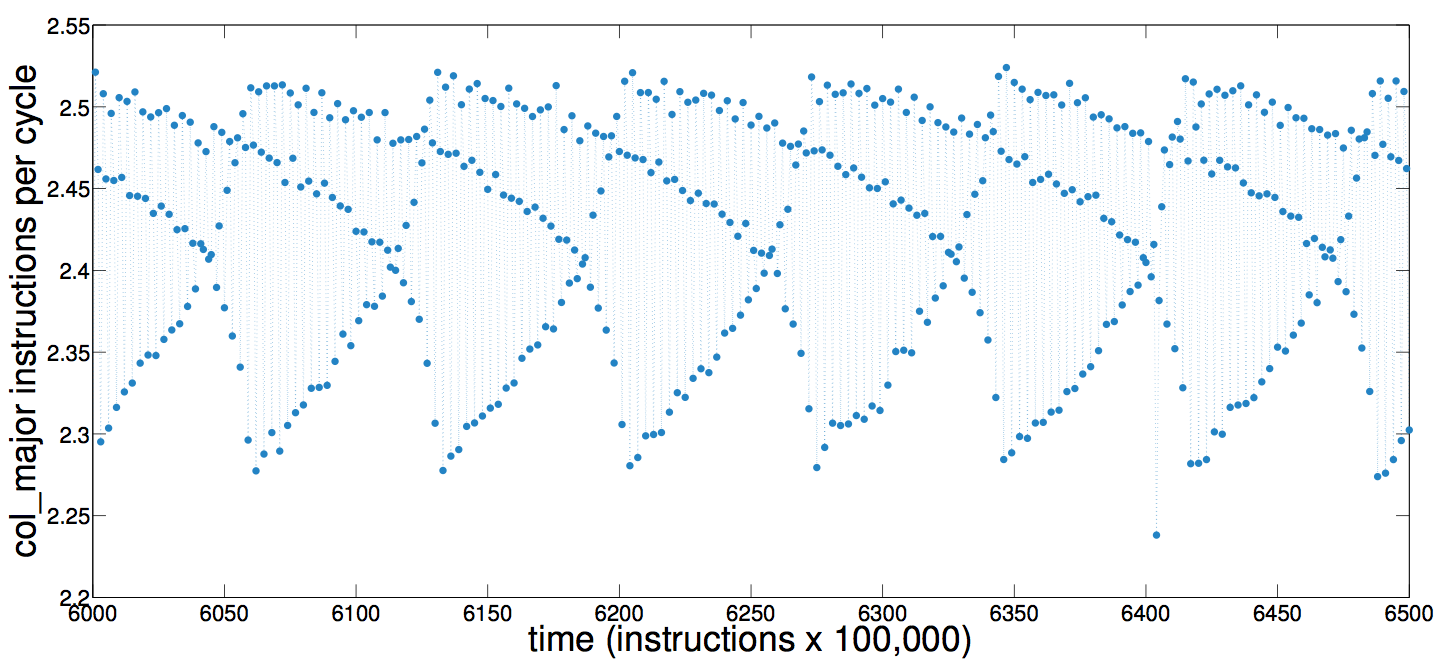
\includegraphics[width=\columnwidth]{figs/colshortts}
    % where an .eps filename suffix will be assumed under latex,
    % and a .pdf suffix will be assumed for pdflatex
    \caption{A computer performance trace: the processor load of \col,
      a simple C program that repeatedly initializes a matrix in
      column-major order, running on an Intel
      i7\textsuperscript{\textregistered}-based machine.}
   \label{fig:col-ipc}
  \end{figure}
%
A small change in the code can cause the dynamics to bifurcate to a
periodic regime.  
% 
% Indeed, many computer performance traces exhibit
% interesting regime changes as a program moves through the different
% phases of its operation.
By running different programs on the same computer, then, we can
produce traces that span the whole range of the complexity spectrum,
from completely predictable to completely unstructured---which makes
this an ideal testbed for this study\footnote{Predicting the
  \emph{state} of a computer, of course, would amount to solving the
  halting problem.  What we are doing here is predicting computer
  \emph{performance}, which does not violate the Rice-Shapiro
  theorem~\cite{hopcroft2007}.}.
% footnote to appease the theoretician in Josh


%The computer systems community has applied a variety of prediction
%strategies to traces like this, most of which employ regression.  An
%appealing alternative builds on the recently established fact that
%computers can be effectively modeled as deterministic nonlinear
%dynamical systems \cite{mytkowicz09}.  This result %implies the
%existence of a deterministic forecast rule for those %dynamics.  In
%particular, one can use \emph{delay-coordinate %embedding} to
%reconstruct the underlying dynamics of computer %performance, then use
%the resulting model to forecast the future values of computer
%performance metrics such as memory or processor loads
%\cite{josh-ida2011}.  In the case of simple microkernels like the one
%that produced the trace in Figure~\ref{fig:ipc}, this deterministic
%modeling and forecast strategy works very well.  In more-complicated
%programs, however, such as numerical software or compilers,
%this forecast strategy---as well as the traditional methods---break
%down some of the time, but work fine others.

%We argue that \emph{permutation entropy}
%\cite{bandt2002per}, a method for measuring the %entropy of a
%real-valued-finite-length time series through ordinal %analysis, is an
%effective way to explore that conjecture.  %{\color{red} Probably remove this and move a%s it is in the experimental methods or point to that section for more details}We study three
%examples---a simple microkernel and two complex %programs: one from the
%SPEC 2006CPU benchmark suite, and one from LAPACK---%running on an Intel i7-based machine.  For
%each program, we calculate the permutation entropy of %the processor
%load (instructions per cycle), then compare that to %the prediction accuracy attainable for
%that trace using a series of deterministic models.

The rest of the paper is organized as follows.
Section~\ref{sec:related} discusses previous results on generating
partitions, local modeling, and error distribution analysis, and
situates this work in that context. Section~\ref{sec:methods} covers
the experimental setup and methods used to collect each time
series. Section~\ref{sec:model} describes the prediction models used
in this study.  Section~\ref{sec:meaComplex} reviews permutation
entropy, the technique that we use to measure complexity.  In
Section~\ref{sec:results}, we estimate the complexity of each
empirical time series and compare that complexity to the accuracy of
predictions produced by the methods of Section~\ref{sec:model},
operating on that time series.  In Section~\ref{sec:conc}, we discuss
these results and their implications, and consider future areas of
research.



\section{Related Work }\label{sec:related}

Modeling time-series data for the purposes of prediction dates back at
least to Yule's 1927 invention of autoregression~\cite{Yule27}.  Since
then hundreds, if not thousands, of strategies have been developed for
a wide variety of prediction tasks.  The purpose of this paper is not
to add a new weapon to this arsenal, nor to assess or compare the
effectiveness of existing methods.  Our goals are more general: {\sl
  (i)} to empirically quantify the predictive structure that is
present in a real-valued scalar time series and {\sl (ii)} to explore
how the performance of prediction methods is related to that inherent
complexity.  It would, of course, be neither practical nor interesting
to report results for every existing forecast method; instead, we
choose a representative set, as described in Section~\ref{sec:model}.

Quantifying predictability, which is sometimes called ``predicting
predictability,'' is not a new problem.  Most solutions to it fall
into two categories: model-based error analysis and model-free
information analysis.
%
%Actually this first class are both just analyzing model error distributions but some are local and some are global models but both are really just error
%
%predicting local predictive capacity (radial basis functions stuff, trying to predict error bounds on next forecast based on ensemble uncertainty) but does not aggregate tell you at what level the time series exhibits complexity only locally predictive structure, this actualy gets at the interesting point that different regions of a time series may exhibit differnt levels of complexity which we will illustrate with \svd
%
The first class focuses on errors produced by a fixed forecasting
schema.  This analysis can proceed locally or globally.  The local
version approximates error distributions for different regions of a
time-series model using local ensemble in-sample
forecasting\footnote{The terms ``in sample'' and ``out of sample'' are
  used in different ways in the forecasting community.  Here, we
  distinguish those terms by the part of the time series that is the
  focus of the prediction: the observed data for the former and the
  unknown future for the latter.  In-sample forecasts---comparisons of
  predictions generated from \emph{part} of the observed time
  series---are useful for assessing model error and prediction
  horizons, among other things.}.
%
These distributions are then used as estimates of out-of-sample
forecast errors in those regions.  For example, Smith {\sl et al.}
make in-sample forecasts using ensembles around selected points in
order to predict the local predictability of that time
series~\cite{Smith199250}.  This approach can be used to show that
different portions of a time series can exhibit varying levels of
local predictive uncertainty.  We expand on this finding later in this
paper with a time series that exhibits interesting regime shifts.

Local model-based error analysis works quite well, but it only
approximates the \emph{local} predictive uncertainty \emph{in relation
  to a fixed model}.  It cannot quantify the inherent predictability
of a time series and thus cannot be used to draw conclusions about
predictive structure that may be usable by other forecast methods.
%
%Distrubtion of error. For many methods, if your error is not normally distributed this signals that there is stil more predictve structure to that could be used by for example a larger order ARMA process. But if error is normally distributed, this suggests that you have used up all the predictive structure that **that** model can use, this doesn't quantify if preidctuce structure exists that isn't being used by this process. For example, nonlinear structure which is ignored by a linear predictor.
%
Global model-based error analysis moves in this direction.  It uses
out-of-sample error distributions, computed \emph{post facto} from a
class of models, to determine which of those models was best.  After
building an autoregressive model, for example, it is common to
calculate the errors and verify that they are normally distributed.
If they are not, that indicates that there is structure in the time
series that the model-building process was unable to capture and use.
The problem with this approach is lack of generality.  
\label{page:normal-errors}
Normally distributed errors indicate that a model has captured the
structure in the data insofar as is possible, \emph{given the
  formulation of that particular model} (viz., the best possible
linear fit to a nonlinear dataset).  This gives no indication as to
whether another modeling strategy might do better.


A practice known as deterministic/sto\-chas\-tic
modeling~\cite{Casdagli92dvsplots, weigend-book} bridges the gap
between local and global approaches to model-based error analysis.
The basic idea is to construct a series of local linear fits,
beginning with a few points and working up to to a global linear fit
that includes all known points, and then analyze how the average
out-of-sample error changes as a function of number of points in the
fit. The shape of such a graph indicates the amounts of determinism
and stochasticity are present in a time series.

The model-based error analysis methods described in the previous three
paragraphs are based on specific assumptions about the underlying
generating process and knowledge about what will happen to the error
if those assumptions hold or fail.  Model-free information analysis
moves away from those restrictions.  Our approach falls into this
class.  Our goal is to empirically measure the inherent complexity of
a time series, then correlate that complexity with the predictive
accuracy of forecasts made using a number of different methods.  

We build on the notion of \emph{redundancy} that was introduced on
page~\pageref{page:redundancy}, which formally quantifies how
information propagates forward through a time series:
% how much information prior observations of a system lend to future
% values
i.e., the mutual information between the past $n$ observations and the
current one.
% took this out because DCE hasn't been introduced yet: 
% 
% For example,
% this would be the amount of information that delay coordinate
% embedding captures.
The redundancy of i.i.d. random processes is zero, since all
observations are independent of one another.  On the other hand, any
deterministic system---including chaotic ones---has maximal redundancy
and thus can be perfectly predicted if observed for long
enough~\cite{weigend-book}.  In practice, it is quite difficult to
estimate the redundancy of an arbitrary, real-valued time series.
Doing so requires knowing either the Kolmolgorov-Sinai entropy or the
values of all positive Lyapunov exponents of the system.  Both of
these calculations are difficult---the latter particularly so if the
data are very noisy or the generating system is stochastic.

Using entropy and redundancy to quantify the inherent predictability
of a time series is not a new idea.  Past methods for this, however,
(e.g.,~\cite{Shannon1951, mantegna1994linguistic}) have hinged on
knowledge of the \emph{generating partition} of the underlying
process, which lets one transform real-valued observations into
symbols in a way that preserves the underlying dynamics~\cite{lind95}.
Different projections---e.g., simply binning the data---can create
spurious complexity in the resulting symbolic sequence and thus
misrepresent the entropy of the underlying system~\cite{bollt2001}.
Generating partitions are luxuries that are rarely, if ever, afforded
to an analyst, since one needs to know the underlying dynamics in
order to construct one.  And even if the dynamics are known, these
partitions are difficult to compute and often have fractal
boundaries~\cite{eisele1999}.

We sidestep these issues by using a variant of the \emph{permutation
  entropy} of Bandt and Pompe~\cite{bandt2002per} to estimate a value
for the Kolmogorov-Sinai entropy of a real-valued time series---and
thus the redundancy in that data, which is an effective proxy for
predictability.  This differs from existing approaches in a number of
ways.  It does not rely on generating partitions---and thus does not
introduce bias into the results if one does not know the dynamics or
cannot compute the partition.  It makes no assumptions about, and
requires no knowledge of, the underlying generating process: linear,
nonlinear, the Lyapunov spectrum, etc.  These features make our
approach applicable to noisy real-valued time series from all classes
of systems.


\section{Experimental Methods and Time Series Explanations}

 \begin{enumerate}
 \item  Experimental methods: (how we collect the time series and what the times series areThis should be HPM PAPI, which programs we model
\item programs 
\subitem description of \col
\subitem description of \gcc
\subitem description of \svd 
\subitem description of svd regimes
 \end{enumerate}


\subsection{Time Series Collection}

The time-series data for these experiments was collected on an Intel Core\textsuperscript{\textregistered} i7-2600 running the 2.6.38-8 Linux
kernel.  This Nehalem chip has eight cores running at 3.40GHz and a cache size
of 8192 KB.  We studied three example programs---a simple microkernel(\col) and two complex programs: one from the
SPEC 2006CPU benchmark suite(\gcc), and one from LAPACK(\svd), aggregating and measuring the processor load---instructions per cycle (ipc)---at 100,000-instruction intervals.  To record these measurements,
we used the {\tt libpfm4}, via PAPI
\footnote{Performance Application Programming Interface}\cite{papi-website}, which we have instrumented to stop program execution every 100,00-instructions and read the contents of the CPU's onboard hardware performance monitors (HPMs). HPMs are specialty registers built for this purpose. Obviously using a system to measure itself can cause interference but due diligence was put into monitoring the generating process of these time series without interfering with it in a significant way. For an in-depth explanation of this custom-measurement infrastructure as well as discussion on choice of interrupt rate see 
\cite{zach-IDA10,mytkowicz09,todd-phd}.



\subsection{The Programs}
We study three example programs---a simple microkernel(\col) and two complex programs: one from the
SPEC 2006CPU benchmark suite(\gcc), and one from LAPACK(\svd).
\subsubsection{\col}
\col is a simple three-line C program that repeatedly initializes the top half of matrix in column-major order. While this is a very simple program it has been shown to exhibit very complicated behavior. In fact, in \cite{chaos} it was shown 
\subsubsection{\gcc}

\subsubsection{\svd}
\svd brings up a very interesting point: systems change over time. While it is clear in Figure \ref{fig:sample-ts} (a) and (b) that a single system is being observed, it also appears \emph{visually} that the complexity of these two time series is consistent over time, i.e., while they are both complicated they don't appear to increase or decrease in complexity over the range of the program. \svd (seen in Figure \ref{fig:svd-ts-colored}) is different however, at least visually. Figure \ref{fig:svd-ts-colored} is a single trace of \svd from start to finish, however as time progresses it is clear that something drastically changes in the underlying generating process and the structure of the time series is visually very different from section to section. This is caused by the code of \svd moving between different subroutines. We call these changes in \svd dynamics  \emph{\svd regimes} and we have colored each of the six regimes different colors in Figure \ref{fig:svd-ts-colored}. The advantage to splitting \svd into these regimes is to explore how complexity and predictability evolve over time for a system in drift. In Section \ref{sec:wpeRegime} we explore and validate the choice of these visually selected regime windows extending techniques from \cite{cao2004det}. The purpose of this paper is not to rigorously explore regime detection but to explore quantifying complexity of a time series. As such, making this split simply serves as providing 90 unique time series\footnote{Six Regimes with 15 individual runs each.} to explore. For notational convience we refer to these signals as {\tt dgesdd$_i$} with $i \in \{1\dots6\}$ where $i$ corresponds to a regime of \svd. The regimes are labeled from left to right. 



\begin{figure}[htbp]
  \centering
  \begin{subfigure}[t]{\textwidth}
  \centering
    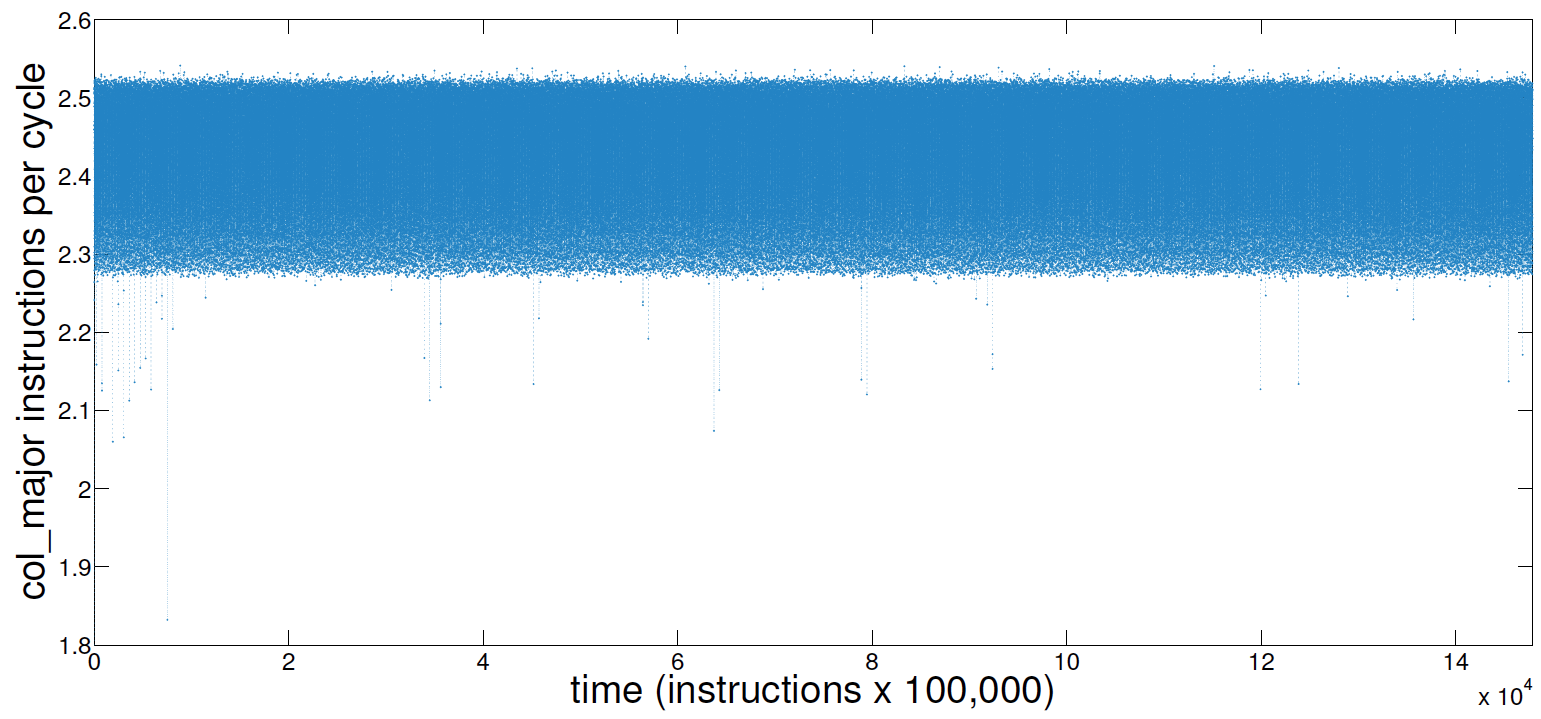
\includegraphics[width=0.75\textwidth]{figs/colFullTS}
    \caption{\col Time Series}
    \label{fig:col-ts}
  \end{subfigure}%
  \\
  
  \begin{subfigure}[t]{\textwidth}
  \centering
    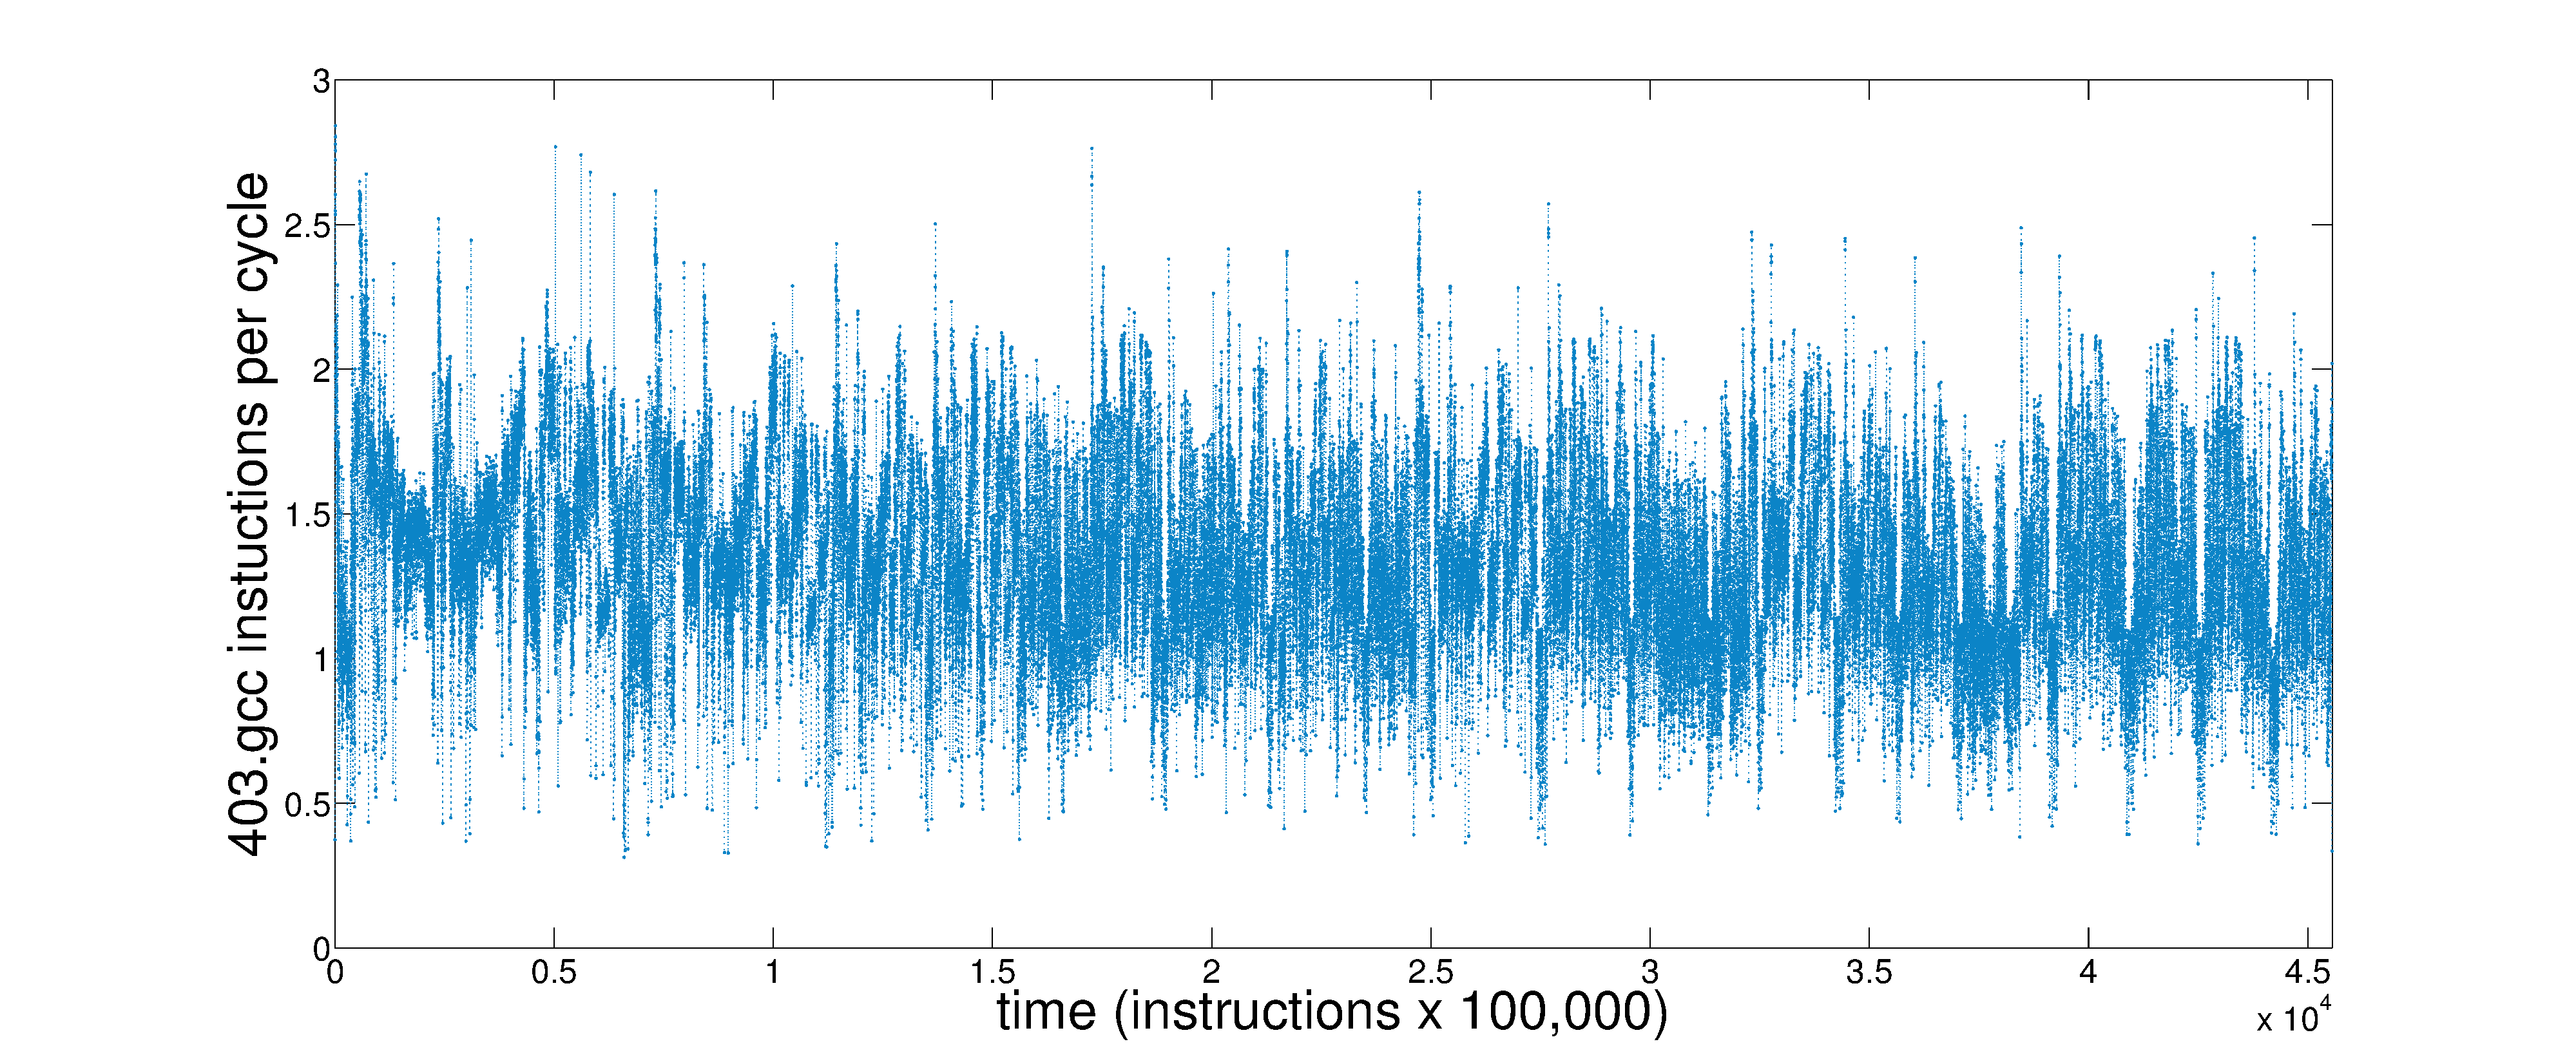
\includegraphics[width=0.75\textwidth]{figs/gccfullts}
    \caption{\gcc Time Series}
    \label{fig:gcc-ts}
  \end{subfigure}
    \begin{subfigure}[t]{\textwidth}
    \centering
    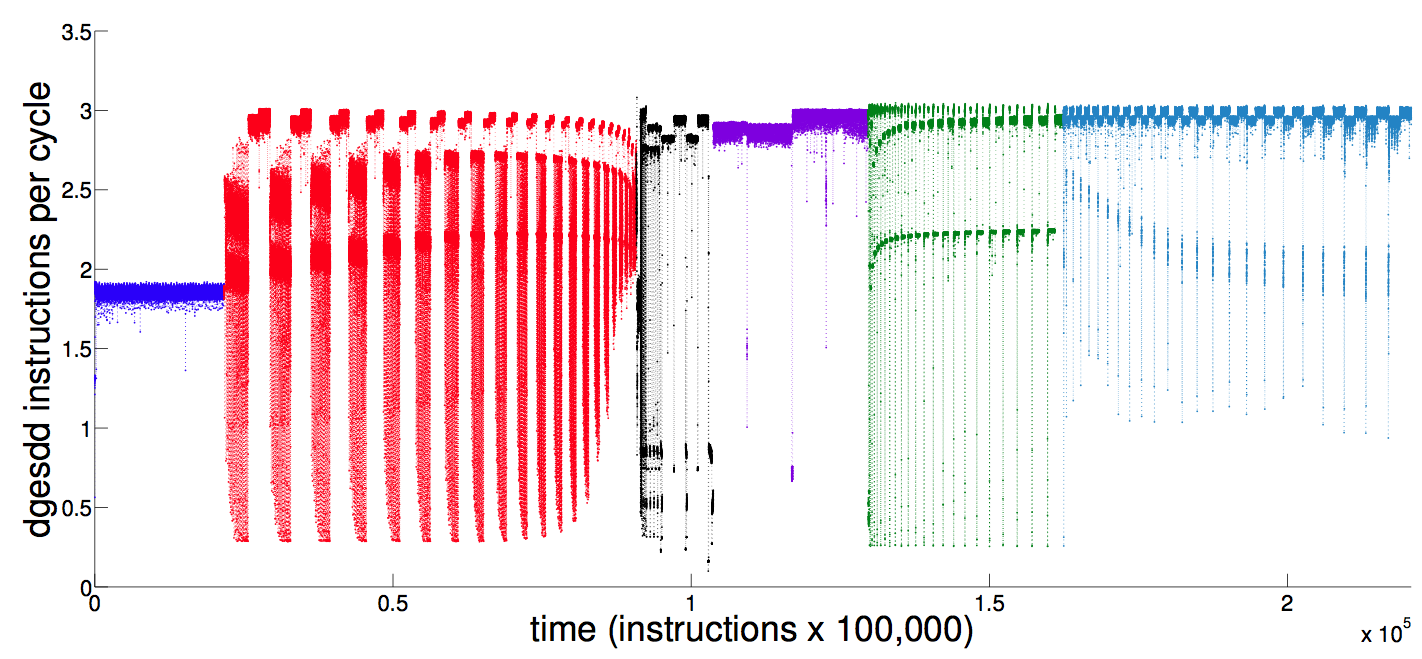
\includegraphics[width=0.75\textwidth]{figs/SVD1RegimesColored}
    \caption{\svd Time Series with Regime Coloring}
    \label{fig:svd-ts-colored}
  \end{subfigure}
  \caption{[[Maybe this should be just a picture of each time series and then have another figure with color after explaining heuristically the reigmes. In (a) the instructions executed per CPU clock cycle
    (IPC) during the execution of \col. Each point is the average IPC during a 100,000
    instruction period. Similarly in (b) is a time series of the IPC during the execution of \gcc.}\label{fig:sample-ts}
    \end{figure}


\section{Modeling }\label{sec:model}
%
% {\color{blue} EDITABLE}
%
% Section outline:
%
% \begin{enumerate}
% \item \cmark section intro
% \item \cmark fix order from simplest to most complex
% \item Description of DCE and parameter estimation
% \item\cmark Description of auto ARIMA
% \item \cmark Description of the two naive methods (random walk and mean), make sure to explain that these methods are naive and simple but not necessarily bad.
% \item\cmark Add a section talking about evaluation methods i.e., MASE, this text is currently written and just sitting at the beginning of the results.
%
% \end{enumerate}

In this section, we describe the four different forecasting methods
used in this study, as well as the error metric used to evaluate their
predictive accuracy.  These methods include:
\begin{itemize}
\item The \emph{random-walk} method, which uses the previous value in
  the observed signal as the forecast,

\item The \emph{\naive} method, which uses the mean of the
  observed signal as the forecast,

\item The \emph{ARIMA} (auto-regressive integrated moving average)
  method, a common linear forecast strategy, and

\item The \emph{LMA} (Lorenz method of analogues) method, which uses a
  near-neighbor forecast strategy on a dynamical reconstruction of the
  signal.
\end{itemize}
ARIMA is based on standard autoregressive techniques.  LMA is designed
to capture and exploit the deterministic structure of a signal from a
nonlinear dynamical system.  The \naive ~and random-walk methods,
somewhat surprisingly, often outperform these more-sophisticated
prediction strategies in the case of highly complex signals, as
discussed below.

\subsection{Two Simple Prediction Strategies}
\label{sec:simple}

A random-walk predictor simply uses the last observed measurement as
the forecast: that is, the predicted value $p_i$ at time $i$ is
calculated using the following relation: $$p_i = x_{i-1}$$ The
prediction strategy that we refer to using the term ``\naive''
averages the prior observations to generate the forecast: $$p_i =
\sum_{j=1}^{i-1}\frac{x_j}{i-1}$$ While both of these methods are
simplistic, they are not without merit.  For a time series near the
high end of the complexity spectrum---i.e., one that possesses very
little predictive structure---these two methods can actually be the
best choice.  In forecasting currency exchange rates, for instance,
sophisticated econometrics-based prediction models fail to
consistently outperform the random-walk method~\cite{rwMeese,rwCCE}.
These signals are constantly changing, noisy, and possess very little
predictive structure, but their variations are not---on the
average---very large, so the random-walk method's strategy of simply
guessing the last known value is not a bad choice.  If a signal has a
unimodal distribution with low variance, the \naive ~prediction
strategy will perform quite well---even if the signal is highly
complex---simply because the mean is a good approximation of the
future behavior.  Moreover, the \naive ~prediction strategy's temporal
average effects a low-pass filtering operation, which can  mitigate the
complexity in signals with very little predictive structure.

Both of these methods have significant weaknesses, however.  Because
they do not model the temporal patterns in the data, or even the
distribution of its values, they cannot track changes in that
structure.  This causes them to fail in a number of important
situations.  Random-walk strategies are a particularly bad choice for
time series that change significantly at every time step.  In the
worst case---a large-amplitude square wave whose period is equivalent
to twice the sample time---a random-walk prediction would be exactly
180 degrees out of phase with the true continuation.  The \naive
~method would be a better choice in this situation, since it would
always split the difference.  It would, however, perform poorly when a
signal has a number of long-lived regimes that have significantly
different means.  In this situation, the inertia of the \naive
~method's accumulating mean is a liability and the agility of the
random-walk method is an advantage, since it can respond quickly to
regime shifts.

Of course, methods that could capture and exploit the geometry of the
data, or its temporal patterns, would be far more effective in the
situations described in the previous paragraph.  The ARIMA and LMA
methods introduced in Sections~\ref{sec:arima} and~\ref{sec:lma} are
designed to do exactly that.
% Note, though, that periodic patterns
%appear only in signals that are at the low end of the %complexity
%spectrum.
However, if a signal contains little predictive structure, forecast
strategies like ARIMA and LMA have nothing to work with and thus will
often be outperformed by the two simple strategies described in this
section.  This effect is explored further in Sections~\ref{sec:accuracy}
and~\ref{sec:results}.


\subsection{A Regression-Based Prediction Strategy}
\label{sec:arima}
%\begin{enumerate}
%\item\cmark introduce method abstractly and practically, common method basically fitting a hyperplane to data removing seasonality and filtering for noise
%\item\cmark define rigorously, all the backshift operator garbage

%$$\Phi(B^m)\phi(B)(1-B^m)^D(1-B)^dX_i = c + \Theta(B^m)\theta(B)\epsilon_i$$

%$$B^mX_i  = X_{i-m}$$
%\item\cmark discuss that this method needs linear structure to work correctly
%\item \cmark maybe talk about converging to zero and limits on prediction horizon
%\end{enumerate}

%For this \cite{davislinearts}

%%%%%%%%%%%%%%%%%%%%%%%%%%%%%%%%%%%%%%%%%%%%%%%%%%%%%%%%%%%%%%%%%%%%%%%%%
% here is the old version of this material, for use in other documents...
%
%Perhaps the simplest way to capture and exploit the structure of data
%is to fit a hyperplane to the dataset and then use that it to forecast
%new data points.  The roots of this date back to Yule's 1927 invention
%of the autoregressive schema~\cite{weigend93}, which forecasts the
%next time step through a weighted average of past observations: $$p_i
%= \phi(B^p)x_{i}$$ where $\phi(\cdot)$ is a polynomial of degree $p$
%that is fit to the past $p+1$ [[???]] values of $x_i$ via the
%backshift operator $B$ \footnote{I changed the superscript to $k$ to
%  make this definition general---not connected to any of the terms
%  that have specific meanings later in this section.}:
%$$B^k x_i = x_{i-k}$$
%%
%with $k=1...p$.  To account for noise in the data, one can add a
%so-called ``moving average'' term to the model:
%$\theta(B^q)\epsilon_i$, where $\theta(\cdot)$ is a polynomial of
%degree $q$ and $\epsilon$ is white noise with the same mean and
%variance as the data.
%% if you leave this in, you'll need to explain a lot about the data
%% and the calculation
%% $\{\epsilon_i\}\sim WN(0,\sigma^2)$.
%To remove nonstationarities in the data, one can detrend it using a
%differencing operation: $(1-B^d)x_i$.
%
%A strategy that incorporates all three of these features is called a
%\emph{nonseasonal ARIMA} model of order $(p,d,q)$:
% $$\phi(B^p)(1-B^d) x_i = \theta(B^q)\epsilon_i$$
%%
%{\color{red} You had superscripts on some of the $B$s and not on
%  others.  I added them but I may have gotten them wrong.  I also
%  changed some $(1-B)^d$s to $(1-B^d)$s to make things consistent with
%  the first use of that construction.  Please make sure things are
%  consistent, here and throughout this section.}  Here, $p$, $d$ and
%$q$ correspond to the orders of the autoregressive, detrending, and
%moving average terms, respectively.
%
%If periodic structure is present in the data, a \emph{seasonal ARIMA}
%model of order $(p,d,q)(P,D,Q)$ can be a good choice:
%%
%$$\Phi(B^P)\phi(B^p)(1-B^m)^D(1-B^d) x_i =
%\Theta(B^Q)\theta(B^q)\epsilon_i$$
%%
%Here $\Phi(\cdot)$ and $\Theta(\cdot)$ are polynomials of degree $P$
%and $Q$, respectively [[which accomplish what purpose?  why?  how?
%    where did $D$ come from and what does it do?]].  $m$ is the
%seasonal frequency [[shouldn't this be ``period''?]].  [[Explain why
%    one should choose $P=Q=m$, since that's what the equation below
%    implicitly does.]]  To use a seasonal ARIMA model, one first uses
%the detrending term to remove nonstationarity: $$\hat{x_i} =
%(1-B^m)^D(1-B^d) x_{i}$$ and then creates the forecast $p_i$ by
%evaluating $$\Phi(B^m)\phi(B^p)\hat{X_i} =
%\Theta(B^m)\theta(B^q)\epsilon_i$$
% ...down to here
%%%%%%%%%%%%%%%%%%%%%%%%

A simple and yet powerful way to capture and exploit the structure of
data is to fit a hyperplane to the dataset and then use it to make
predictions.  The roots of this approach date back to the original
autoregressive schema~\cite{weigend93}, which forecasts the next time
step through a weighted average of past observations: $$p_i =
\sum_{j=1}^{i-1} a_j x_j$$ The weighting coefficients $a_j$ are
generally computed using either an ordinary least squares approach, or
with the method of moments using the Yule-Walker equations.  To
account for noise in the data, one can add a so-called ``moving
average'' term to the model; to remove nonstationarities, one can
detrend the data using a differencing operation.  A strategy that
incorporates all three of these features is called a \emph{nonseasonal
  ARIMA model}.  If evidence of periodic structure is present in the
data, a \emph{seasonal ARIMA model}, which adds a sampling operation
that filters out periodicities, can be a good choice.

There is a vast amount of theory and literature regarding the
construction and use of models of this type; we refer the reader to
\cite{davislinearts} for an in-depth exploration.  For the purposes of
this paper, where the goal is to explore the relationship between
predictability and complexity across a broad array of forecast
strategies, seasonal ARIMA models are a good exemplar of the class of
linear predictors.  Fitting such a model to a dataset involves
choosing values for the various free parameters in the autoregressive,
detrending, moving average, and filtering terms.  We employ the
automated fitting techniques described in~\cite{autoARIMA} to
accomplish this.  This procedure uses sophisticated methods---KPSS
unit-root tests~\cite{KPSSunit}, a customization of the Canova-Hansen
test~\cite{Canova1995}, and the Akaike information
criterion~\cite{akaike1974}, conditioned on the maximum likelihood
of the model fitted to the detrended data---to select good values for
the free parameters of the ARIMA model.

ARIMA forecasting is a common and time-tested procedure.  Its
adjustments for seasonality, nonstationarity, and noise make it an
appropriate choice for short-term predictions of time-series data
generated by a wide range of processes.  If information is being
generated and/or transmitted in a nonlinear way, however, a global
linear fit is inappropriate and ARIMA forecasts can be inaccurate.
Another weakness of this method is prediction horizon: an ARIMA
forecast is guaranteed to converge to the mean after some number of
predictions, depending on model order.  To sidestep this issue, we
build forecasts in a stepwise fashion: i.e., fit the model to the
existing data, use that model to perform a one-step prediction, rebuild it
using the latest observations, and iterate until the desired
prediction horizon is reached.  (For consistency, we take the same
approach with the other three models in this study as well, even
though doing so amounts to artificially hobbling LMA.)

\subsection{A Nonlinear Prediction Strategy}
\label{sec:lma}

When the temporal progressions in a time series are produced by a
deterministic nonlinear process, one can use a technique called
delay-coordinate embedding
%
%% Note: claiming that we can reconstruct the dynamics of the
%% underlying generating process isn't right.  That would be
%% equivalent to solving the system identification problem!  We're
%% not reconstructing the underlying system, just its output.
%
to model the structure of the information generation and transmission
occurring in the underlying process, then use that reconstruction to
generate forecasts.  This section discusses the theory and
implementation of a prediction strategy that is based on this idea.

Delay-coordinate embedding~\cite{packard80,Sauer:1991lr,Takens:1981uq}
allows one to reconstruct a dynamical system's full state-space
dynamics from a scalar time-series measurement---provided that some
conditions hold regarding those data.  Specifically, if the underlying
dynamics and the measurement function---the mapping from the unknown
state vector $\vec{X}$ to the observed value $x_i$---are both smooth
and generic, Takens~\cite{Takens:1981uq} formally proves that the
delay-coordinate map
\[
F(\tau,m)(\vec{X}) = ([x_{i} ~ x_{i+\tau} ~ \dots ~x_{i+m\tau}])
\]
from a $d$-dimensional smooth compact manifold $M$ to
$\mathbb{R}^{2d+1}$ is a diffeomorphism on $M$---in other words, that
the reconstructed dynamics and the true (hidden) dynamics have the
same topology.  This is an extremely powerful result: among other
things, it means that one can model the full system dynamics, up to
diffeomorphism, without measuring---or even knowing---every one of its
state variables.

The first step in the delay-coordinate embedding process is to
estimate values for the two free parameters in the map: the delay
$\tau$ and the dimension $m$.  We follow standard procedures for this,
choosing the first minimum in the time-delayed mutual information as
an estimate of $\tau$~\cite{fraser-swinney} and using the
false-near(est)-neighbor(s) method of~\cite{KBA92} to estimate $m$.
Some example plots of data from
Figures~\ref{fig:col-ts}-\ref{fig:svd-ts-colored}, embedded following
this procedure, are shown in Figure~\ref{fig:embedding}.
 \begin{figure}
   \centering
\begin{subfigure}{\columnwidth}
    \includegraphics[width=\columnwidth]{figs/colipc3d}
    \caption{\col }
    \label{fig:colEmbedding}
  \end{subfigure}%  \\

    \begin{subfigure}{\columnwidth}
    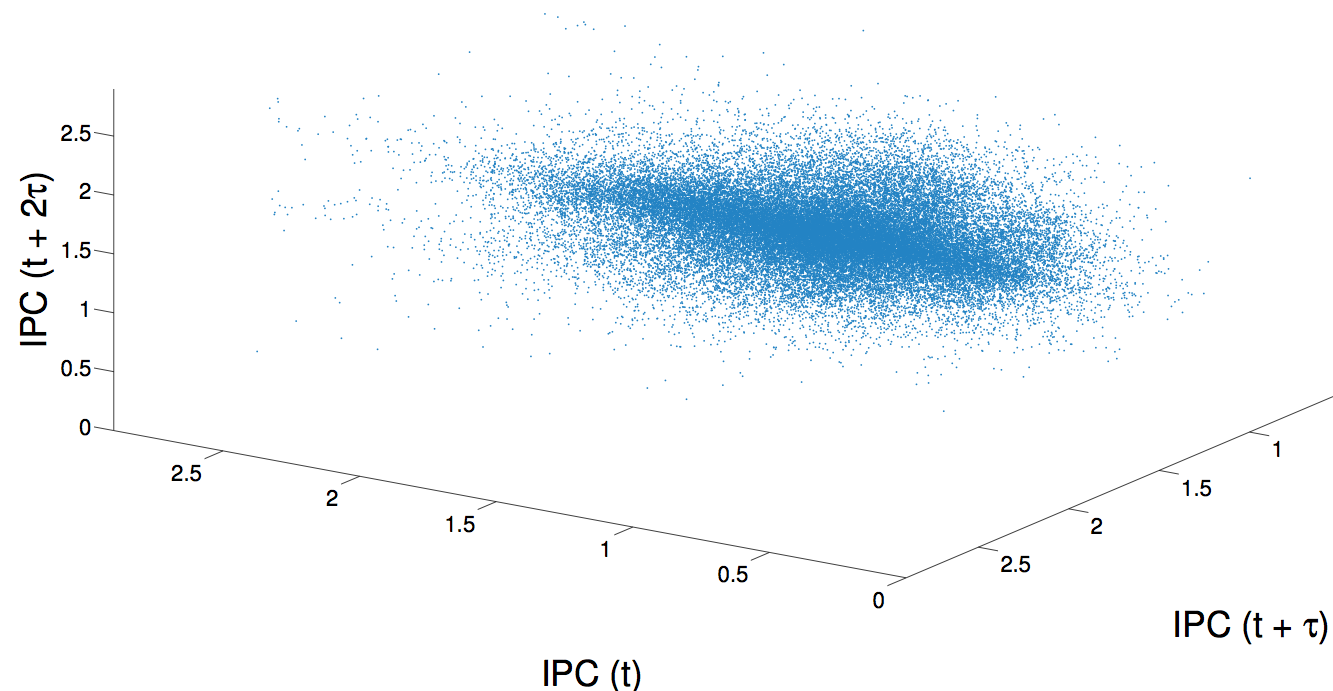
\includegraphics[width=\columnwidth]{figs/gcc3dipc}
    \caption{\gcc}
    \label{fig:gccEmbedding}
  \end{subfigure}
  \\
  \begin{subfigure}{\columnwidth}
    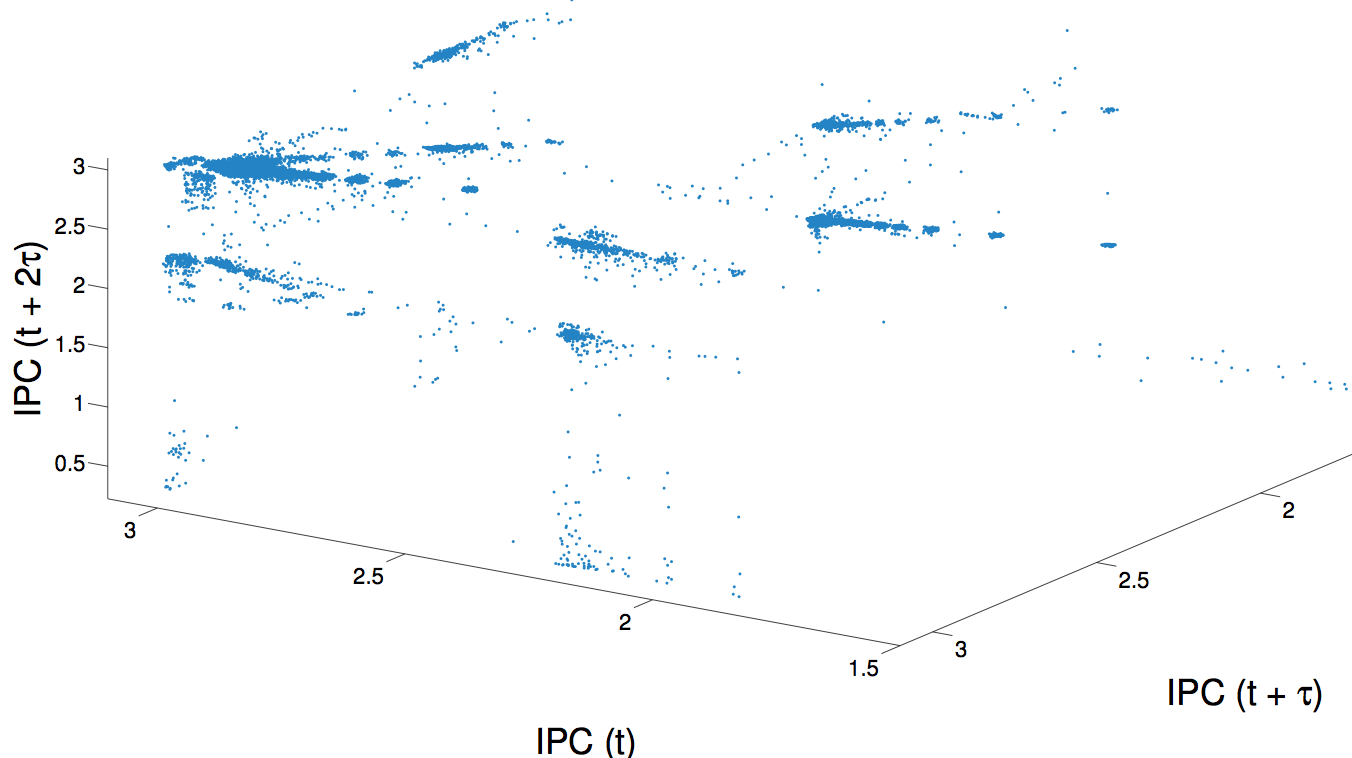
\includegraphics[width=\columnwidth]{figs/svd53dipc2}
    \caption{\svdfive}
    \label{fig:svdfiveEmbedding}
  \end{subfigure}%
%


     %\includegraphics[width=\textwidth]{colipc3d}
     \caption{3D projections of delay-coordinate embeddings of the
       traces from (a) Figure~\ref{fig:col-ts} (b)
       Figure~\ref{fig:gcc-ts} and (c) the fifth (green) segment of
       Figure~\ref{fig:svd-ts-colored}.}
 \label{fig:embedding}
 \end{figure}
%% can cut for space if need be:
%The coordinates of each point in these plots are differently delayed
%elements of the instructions per cycle time series $X_{i,obs}$: that
%is, $X_{i,obs}$ on the first axis, $X_{i+\tau,obs}$ on the second,
%$X_{i+2\tau,obs}$ on the third, and so on.
%

Geometric structure in these kinds of plots is an indication of
structure in the information generation/transmission process that
produced the time series.  The dynamical systems community has
developed a number of methods that leverage this structure to generate
predictions (e.g.,~\cite{weigend-book,casdagli-eubank92,Smith199250}).
One of the most straightforward of these is the \emph{Lorenz method of
  analogues} (LMA), which is essentially nearest-neighbor prediction
in the embedded\footnote{Lorenz's original formulation used the full
  system state space;
%
%According to \cite{kantz97},
%
this method was first extended to embedded dynamics by
Pikovsky~\cite{pikovsky86-sov}, but is also related to the prediction
work of Sugihara \& May~\cite{sugihara90}}
space~\cite{lorenz-analogues}.  Even this simple algorithm---which
builds predictions by finding the nearest neighbor in the embedded
space of the given point, then taking that neighbor's path as the
prediction---provides accurate forecasts when the generating process
is a deterministic dynamical system.

Since LMA does not rest on an assumption of linearity (as ARIMA does),
it can handle both linear and nonlinear processes.  If the underlying
generating process is nondeterministic, however, it can perform
poorly.  In Figure~\ref{fig:embedding}b, for instance, little
structure is visible, so LMA may not work well.  More structure
appears to be present in~Figure~\ref{fig:embedding}c, but this
reconstruction also appears to contain some noise.  The question as to
how much structure is present in a reconstruction---and how much of
that structure can be captured and used by LMA---is apropos of the
central question treated in this paper.  It may be that \gcc has some
redundancy that LMA cannot exploit, or that the structure in \svdfive
is effectively obfuscated, from the standpoint of the LMA method, by
noise.  By quantifying the balance between redundancy (that is,
predictive structure) and entropy for these real-valued time series,
as shown in Section~\ref{sec:results}, we can begin to answer these
questions.

% If enough predictive structure is present in these embeddings, that
% structure can be used to build an effective forecast model.

\subsection{Assessing Prediction Accuracy}
\label{sec:accuracy}

To study the relationship between predictability and complexity, we
use the four methods outlined above to generate predictions of all 360
traces described in Section~\ref{sec:methods}, then calculate the
error of the predictions with respect to the true continuations.
Specifically, we split each time series into two pieces: the first
90\%, referred to as the ``initial training" signal and denoted
$\{x_i\}_{i=1}^{n}$, and the last 10\%, known as the ``test" signal
$\{c_j\}_{j=n+1}^{k+n+1}$.  The initial training signal is used to
build the model, following the procedures described in the previous
section; that model is used to generate a prediction of the value of
$x_{n+1}$, which is then compared to the true continuation, $c_{n+1}$.
The model is then rebuilt using $\{x_i\}_{i=1}^{n+1}$ and the process
repeats $k$ times, out to the end of the observed time series.  This
``one step prediction'' process is not technically necessary in the
LMA method, whose ability to generate accurate predictions is limited
only by the positive Lyapunov exponents of the system.  However, the
performance of the other three methods used here will degrade severely
if the associated models are not periodically rebuilt.  In order to
make the comparison fair, we used an iterative one-step prediction
schema \emph{for all four methods}.  This has the slightly confusing
effect of causing the ``test'' signal to be used both to assess the
accuracy of each model and for periodic refitting.

Figure~\ref{fig:forecast-example} shows example forecasts made using
all four methods for the \col, \gcc, and \svdfive time series.
\begin{figure*}[htbp]
  \centering

  \begin{subfigure}{0.6\columnwidth}
    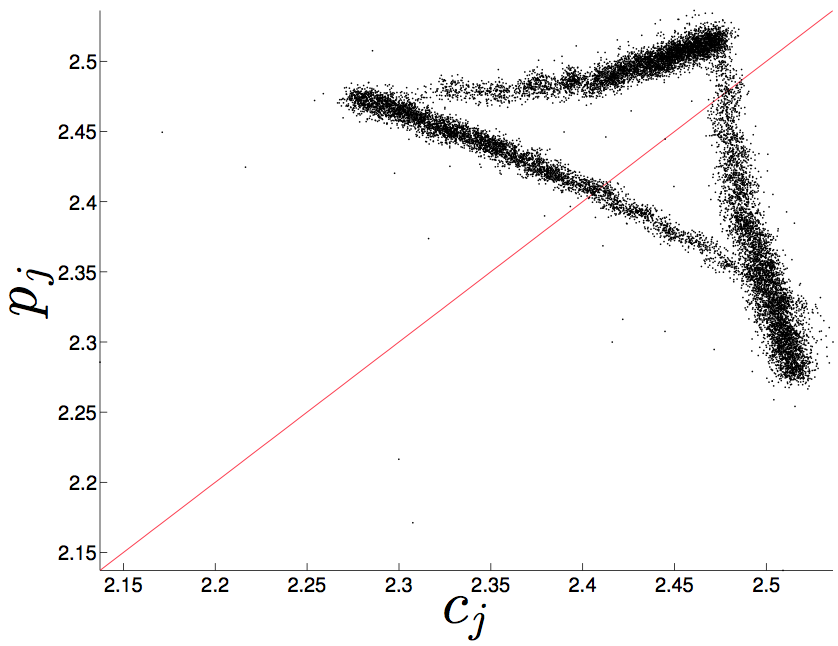
\includegraphics[width=\columnwidth]{figs/colRWForecast}
    \caption{\col\\ random walk }
    \label{fig:colRW}
  \end{subfigure}%
   \begin{subfigure}{0.6\columnwidth}
    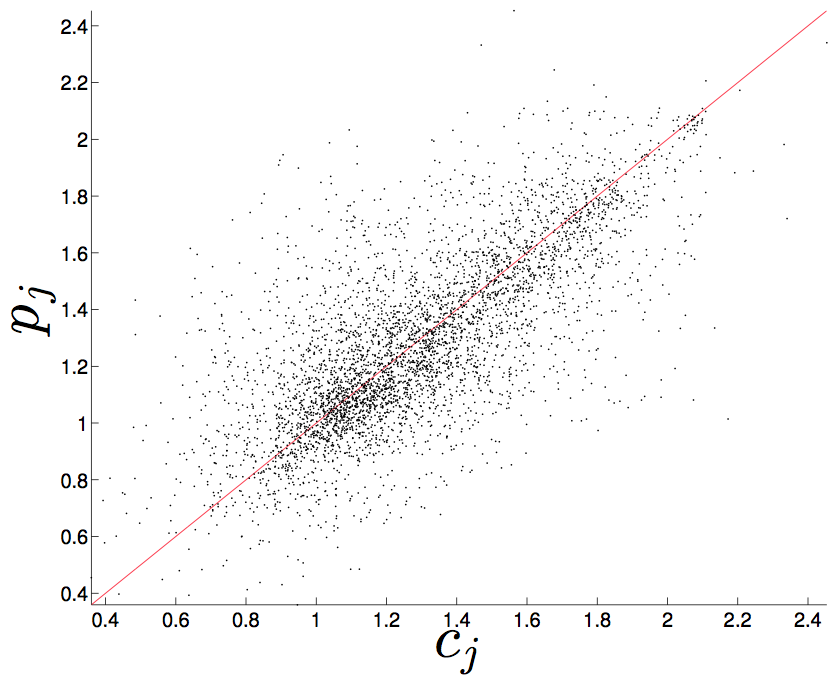
\includegraphics[width=\columnwidth]{figs/gccRWForecast}
    \caption{\gcc\\ random walk }
    \label{fig:gccRW}
  \end{subfigure}%
     \begin{subfigure}{0.6\columnwidth}
    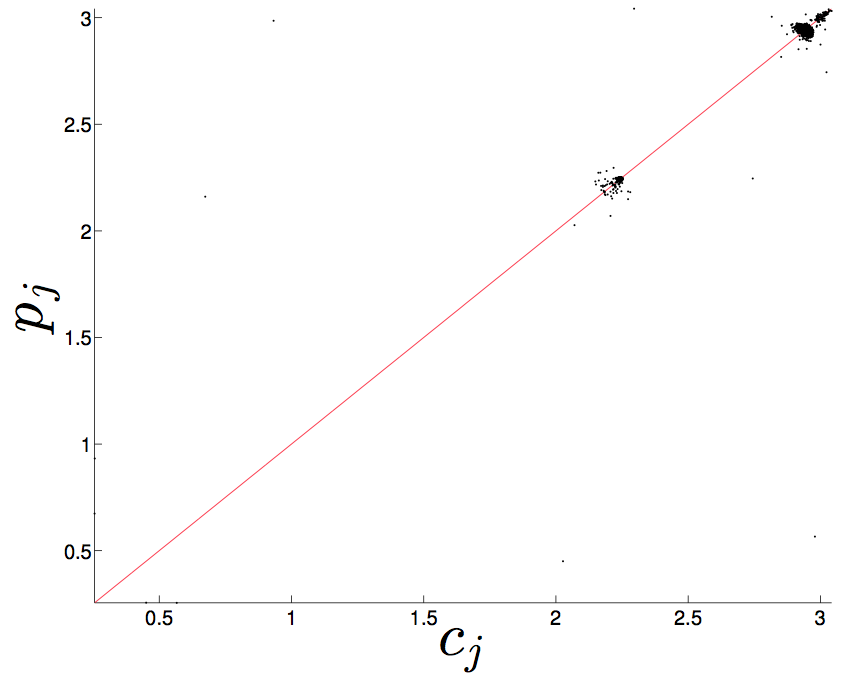
\includegraphics[width=\columnwidth]{figs/svdfiveRWForecast}
    \caption{\svdfive\\ random walk}
    \label{fig:svd5RW}
  \end{subfigure}%
  \\
      \begin{subfigure}{0.6\columnwidth}
    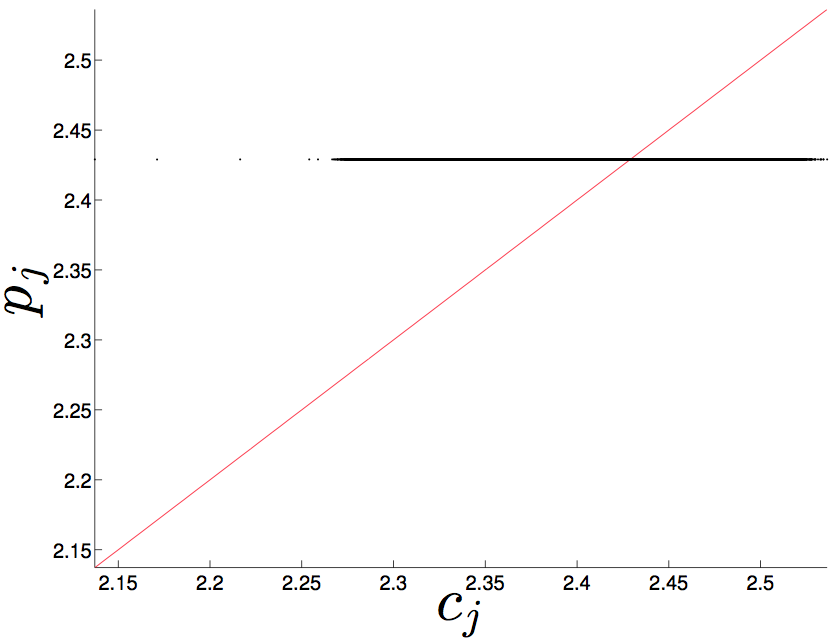
\includegraphics[width=\columnwidth]{figs/colMeanForecast}
    \caption{\col\\ na\"ive }
    \label{fig:colMEAN}
  \end{subfigure}%
   \begin{subfigure}{0.6\columnwidth}
    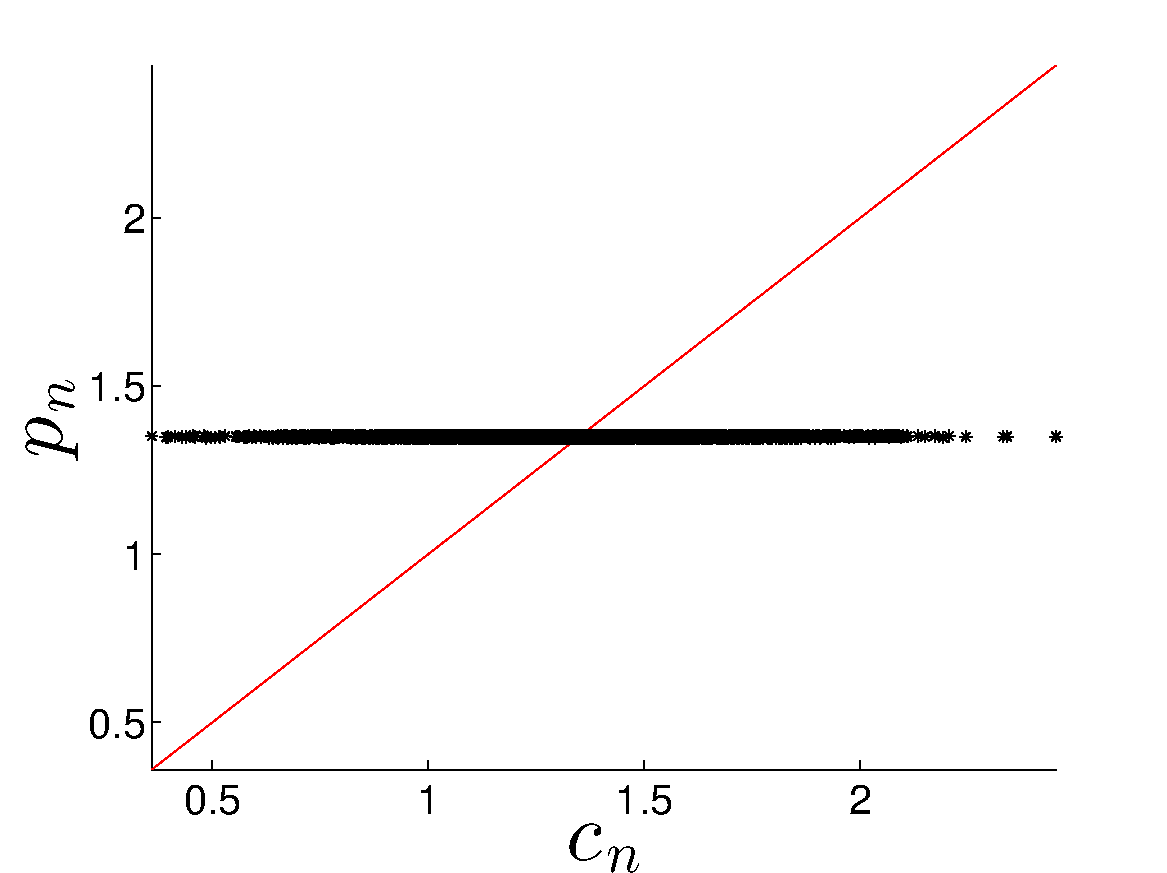
\includegraphics[width=\columnwidth]{figs/gccMeanForecast}
    \caption{\gcc\\ na\"ive }
    \label{fig:gccMEAN}
  \end{subfigure}%
     \begin{subfigure}{0.6\columnwidth}
    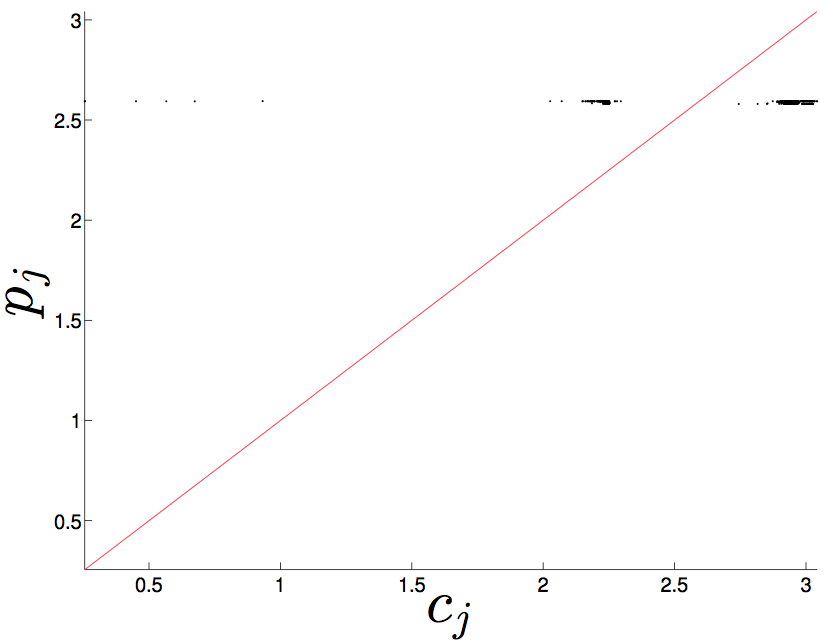
\includegraphics[width=\columnwidth]{figs/svdfiveMeanForecast}
    \caption{\svdfive\\ na\"ive }
    \label{fig:svd5MEAN}
  \end{subfigure}%
  \\
    \begin{subfigure}{0.6\columnwidth}
    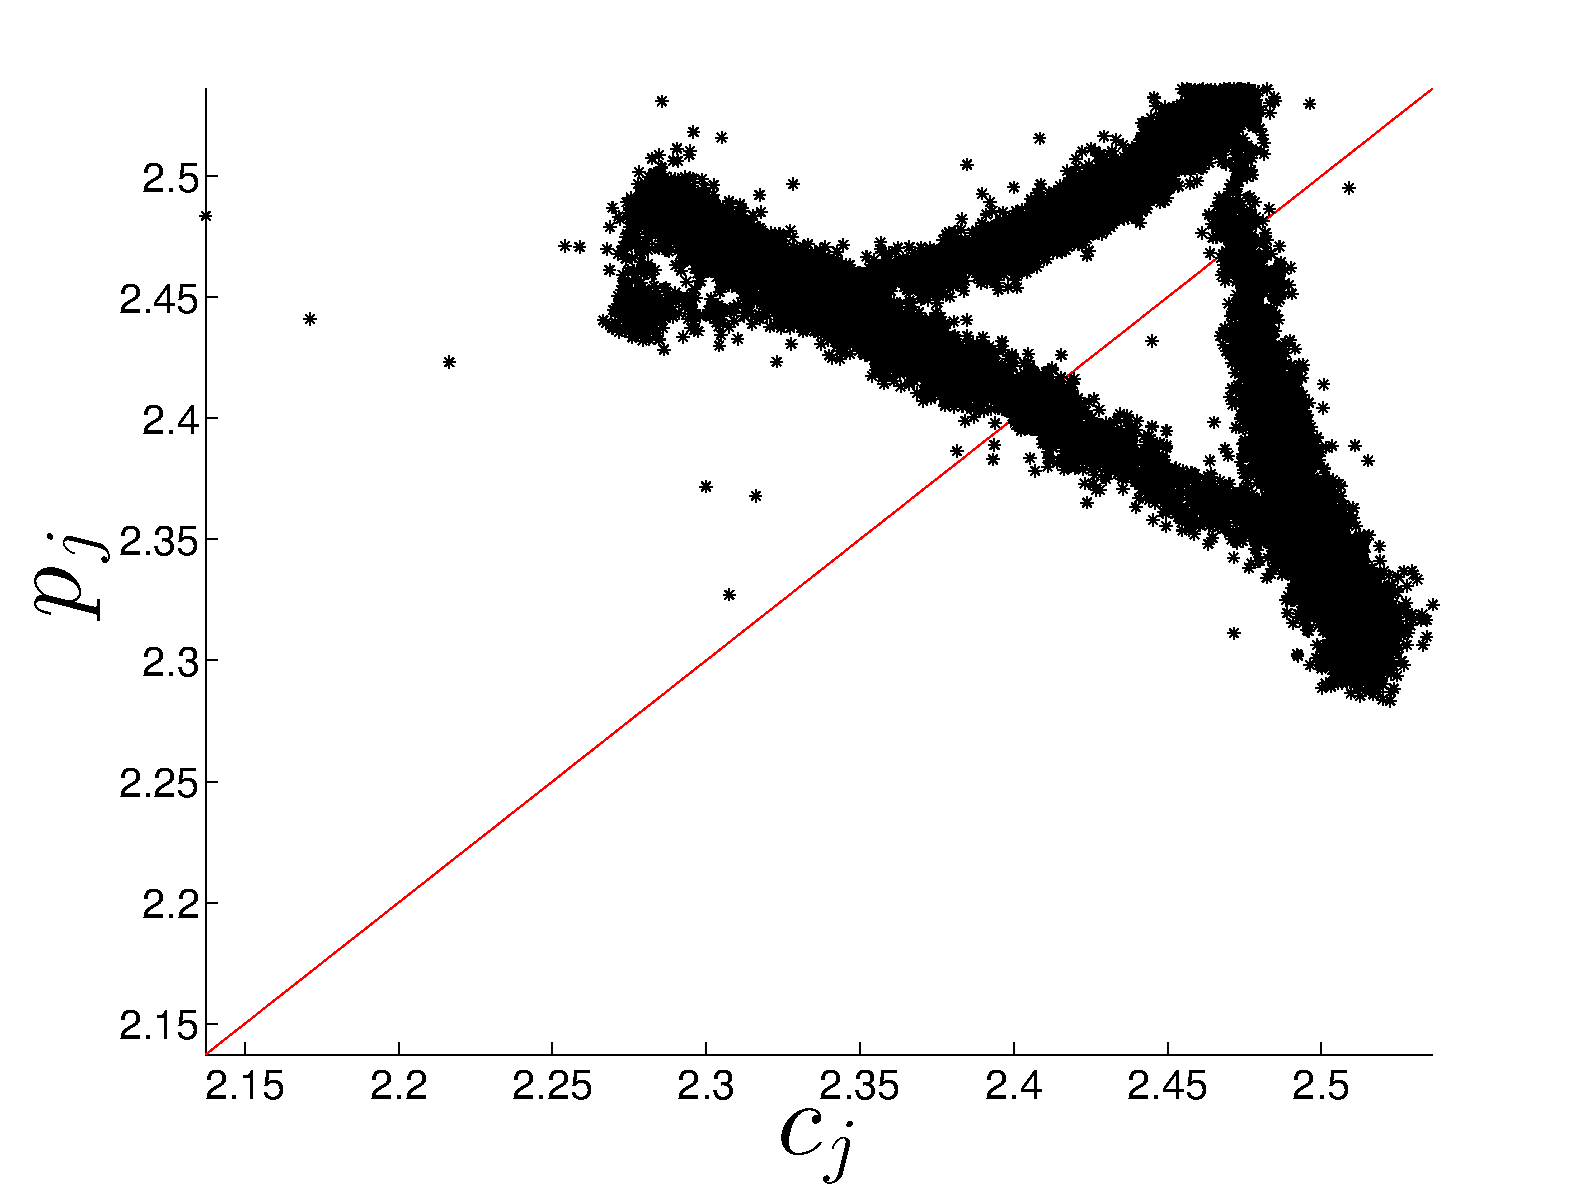
\includegraphics[width=\columnwidth]{figs/colARIMAForecast}
    \caption{\col \\ ARIMA}
    \label{fig:colARIMA}
  \end{subfigure}
  \begin{subfigure}{0.6\columnwidth}
    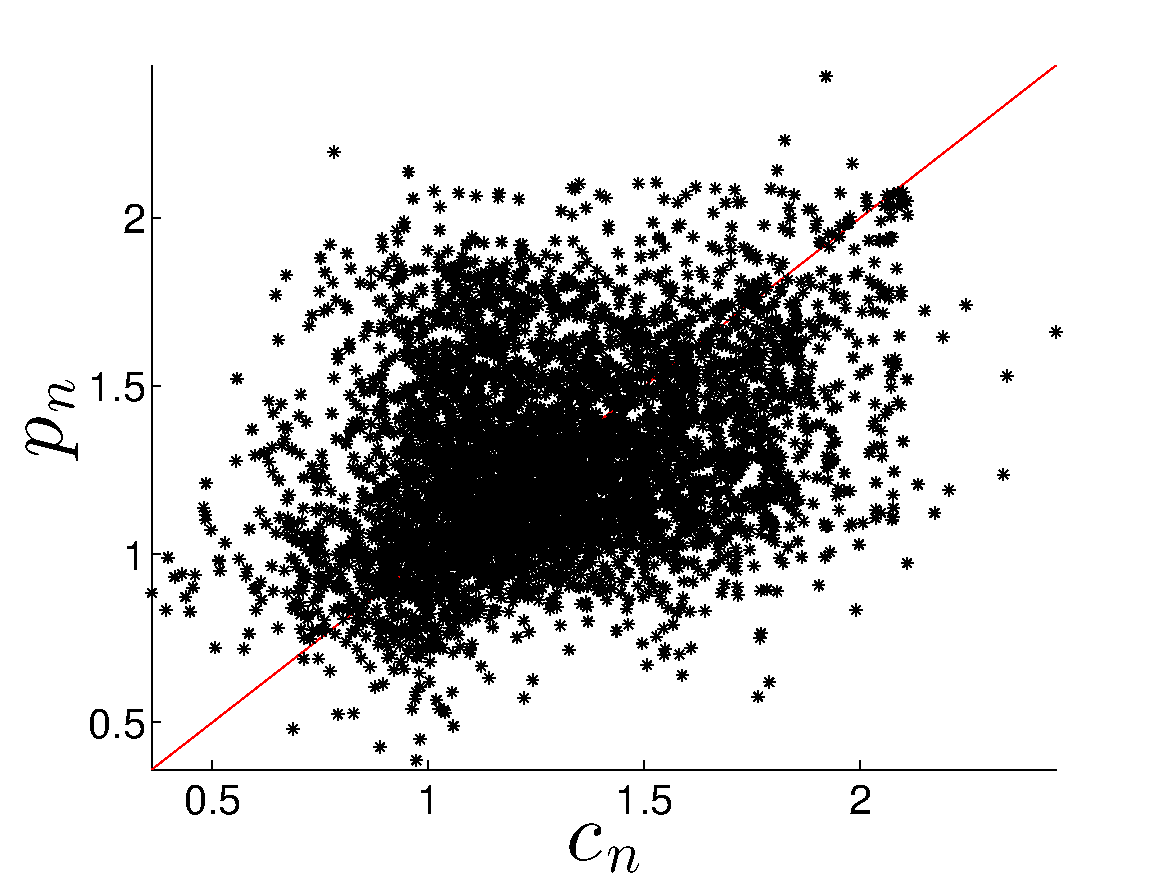
\includegraphics[width=\columnwidth]{figs/gccARIMAForecast}
    \caption{\gcc \\ ARIMA }
    \label{fig:gccARIMA}
  \end{subfigure}%
  \begin{subfigure}{0.6\columnwidth}
    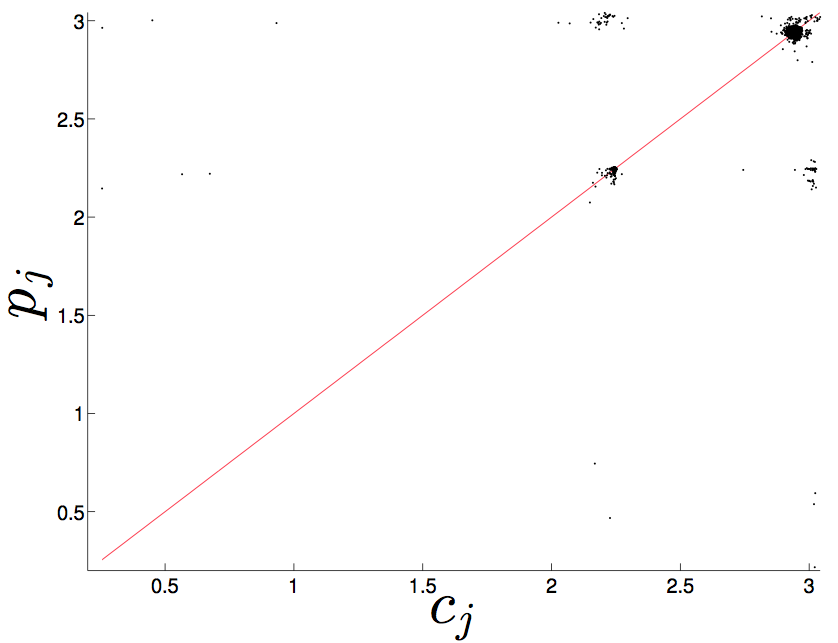
\includegraphics[width=\columnwidth]{figs/svdfiveARIMAForecast}
    \caption{\svdfive \\ ARIMA }
    \label{fig:svd5ARIMA}
  \end{subfigure}%
  \\

      \begin{subfigure}{0.6\columnwidth}
    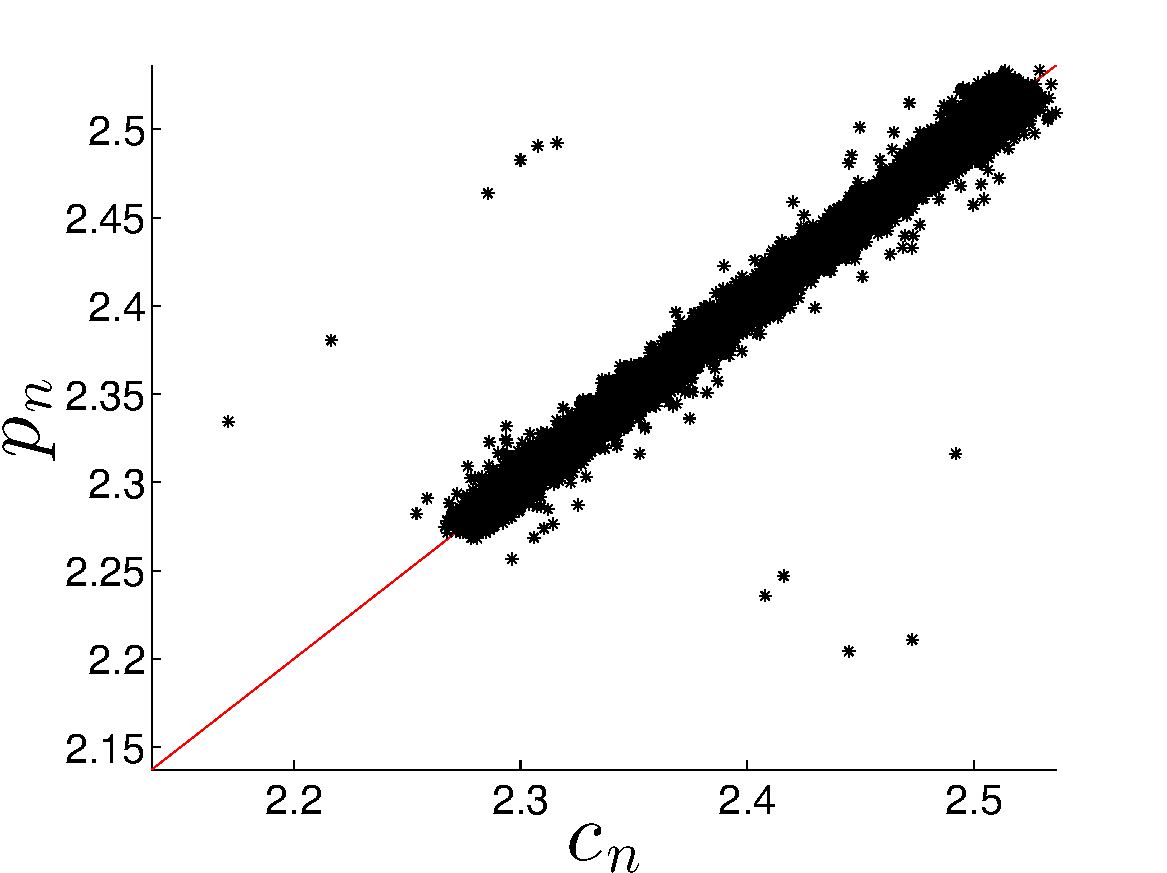
\includegraphics[width=\columnwidth]{figs/colLMAForecast}
    \caption{\col \\ LMA}
    \label{fig:colLMA}
  \end{subfigure}
      \begin{subfigure}{0.6\columnwidth}
    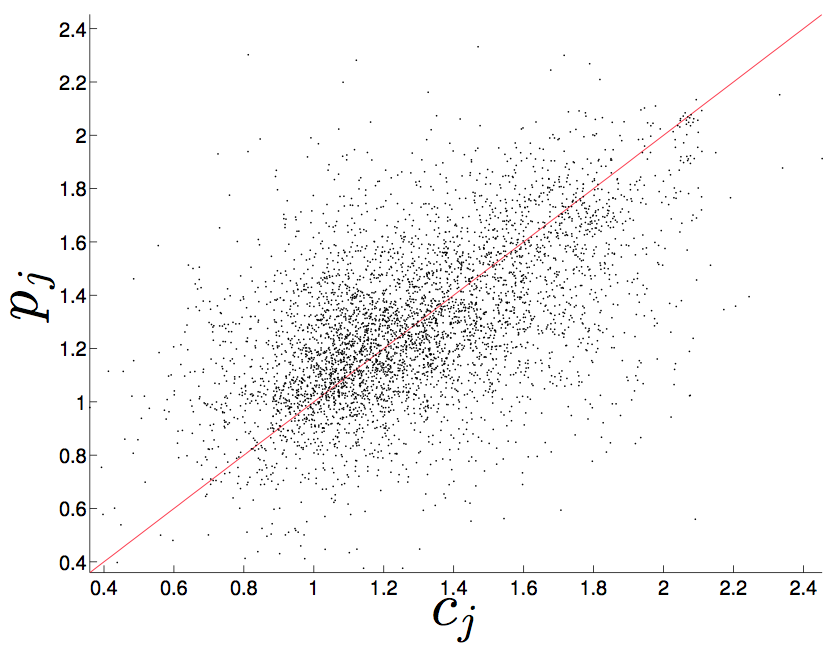
\includegraphics[width=\columnwidth]{figs/gccLMAForecast}
    \caption{\gcc \\ LMA}
    \label{fig:gccLMA}
  \end{subfigure}
        \begin{subfigure}{0.6\columnwidth}
    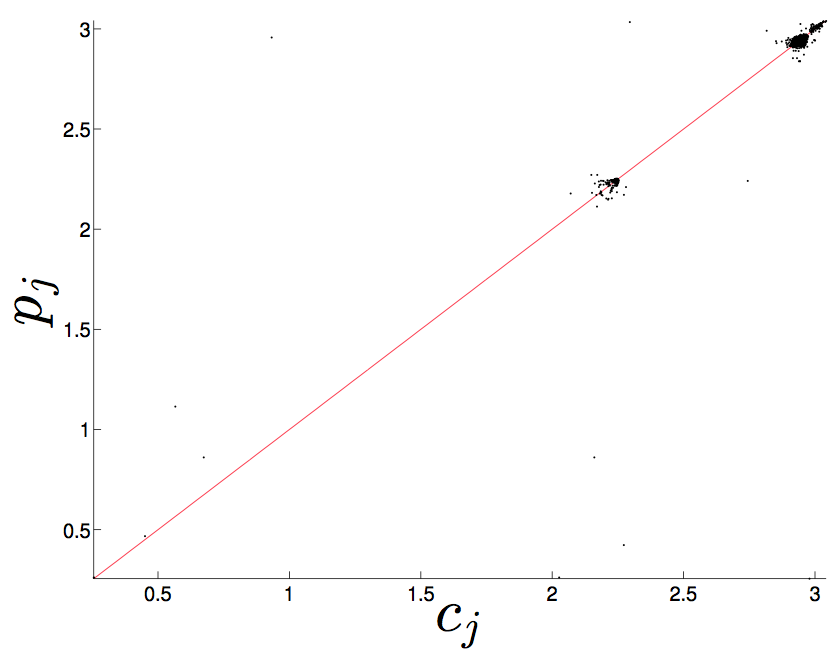
\includegraphics[width=\columnwidth]{figs/svdfiveLMAForecast}
    \caption{\svdfive \\ LMA}
    \label{fig:svd5LMA}
  \end{subfigure}
  %\begin{subfigure}{0.5\textwidth}
  %  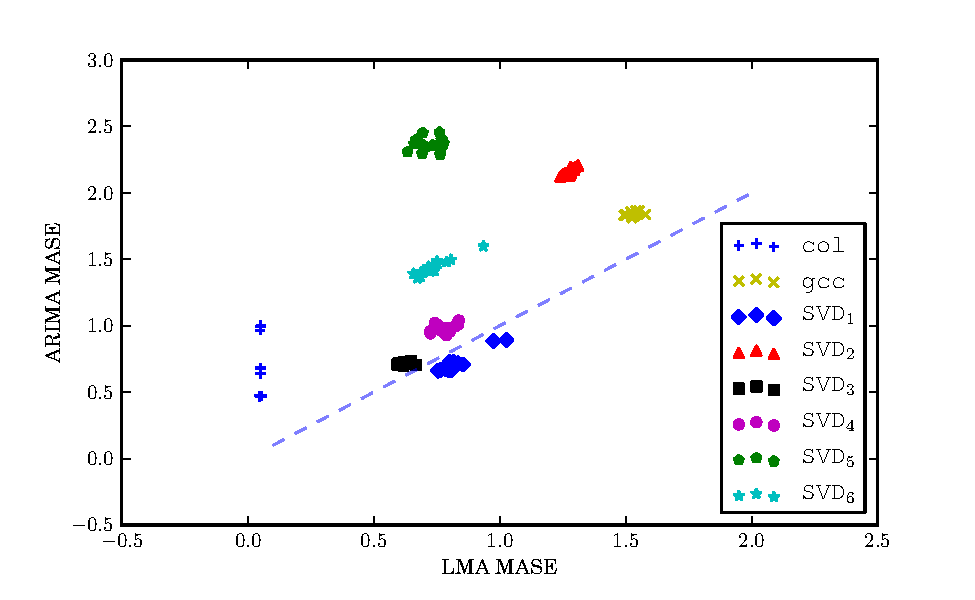
\includegraphics[width=1.0\textwidth]{LMA_vs_ARIMA}
   \caption{Predicted ($p_j$) versus true values ($c_j$) for
     forecasts of \col, \gcc, and \svdfive and all four prediction strategies.
% On this type of plot, a perfect prediction lies exactly on the
% diagonal.
%
%
}
\label{fig:forecast-example}
  %\end{subfigure}
\end{figure*}

\begin{table*}
  \renewcommand{\arraystretch}{1.25}
  \begin{tabular}{lccc}
    & {\large \col} & {\large \gcc} & {\large \svdfive} \\
    & & & \\
    \begin{sideways}\large random walk\end{sideways} &
    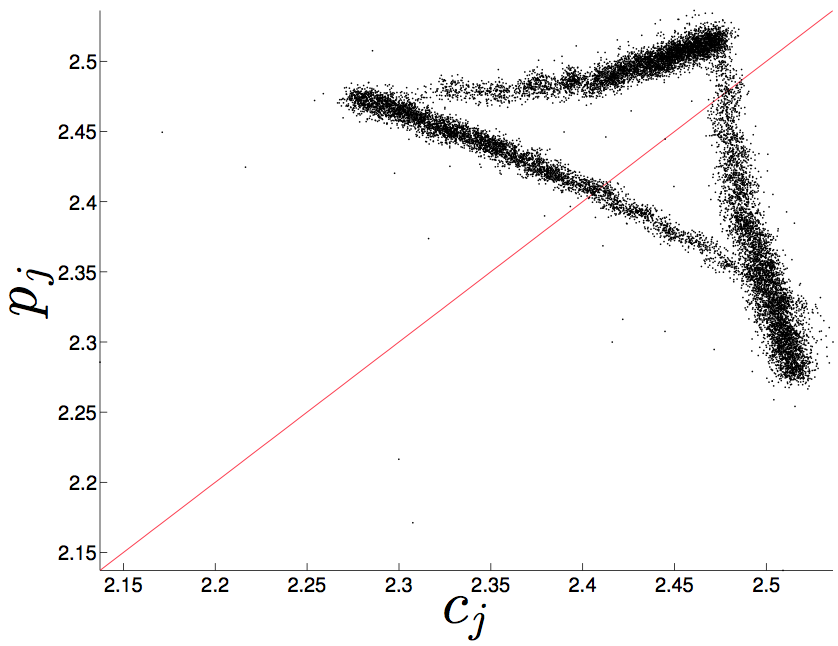
\includegraphics[width=0.6\columnwidth]{figs/colRWForecast} &
    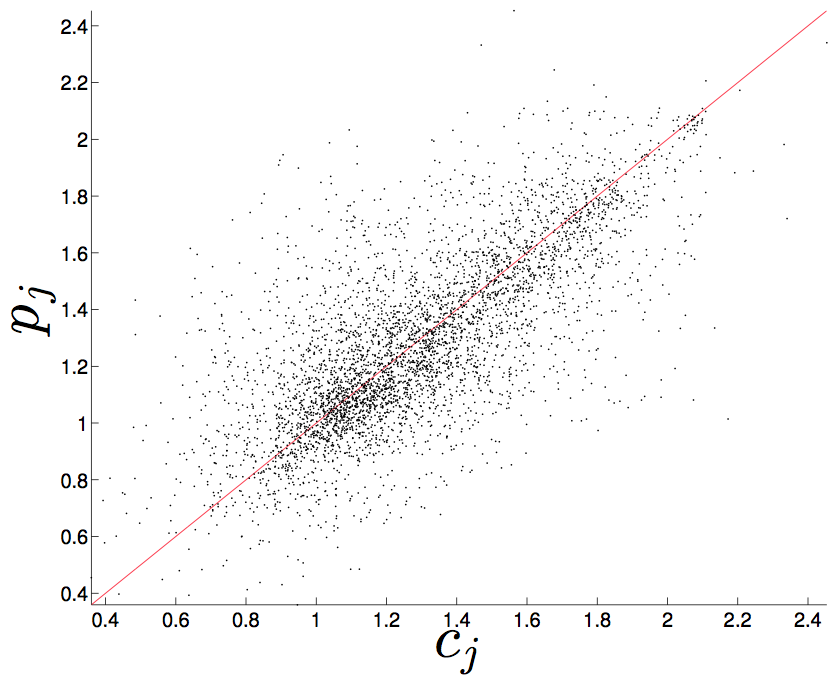
\includegraphics[width=0.6\columnwidth]{figs/gccRWForecast} &
    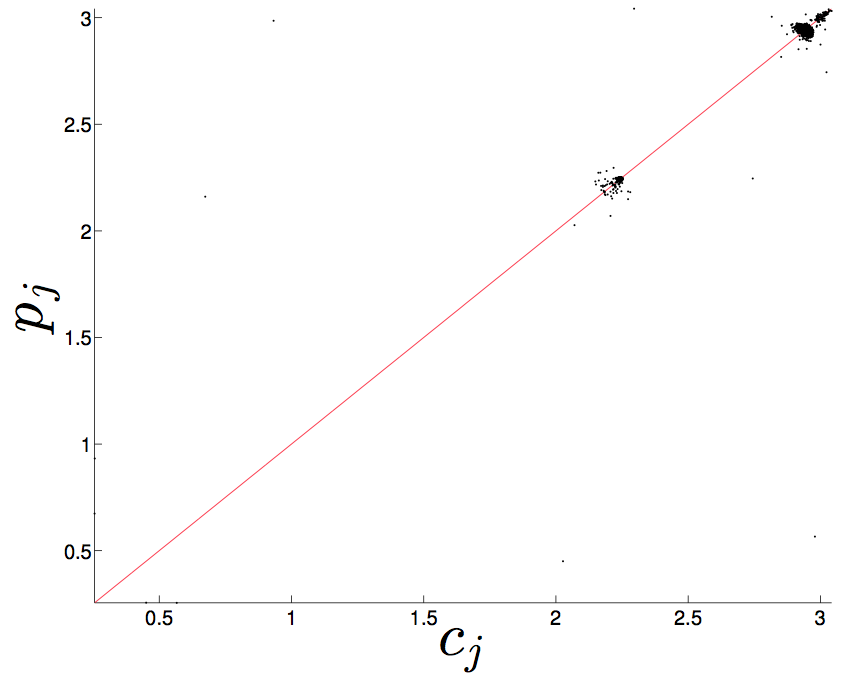
\includegraphics[width=0.6\columnwidth]{figs/svdfiveRWForecast} \\
    \begin{sideways}\large na\"ive\end{sideways} &
    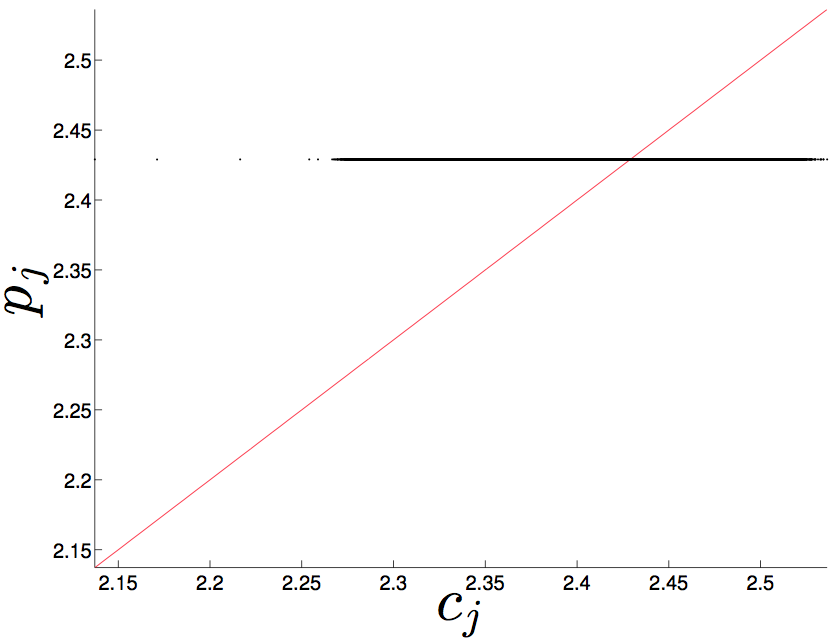
\includegraphics[width=0.6\columnwidth]{figs/colMeanForecast} &
    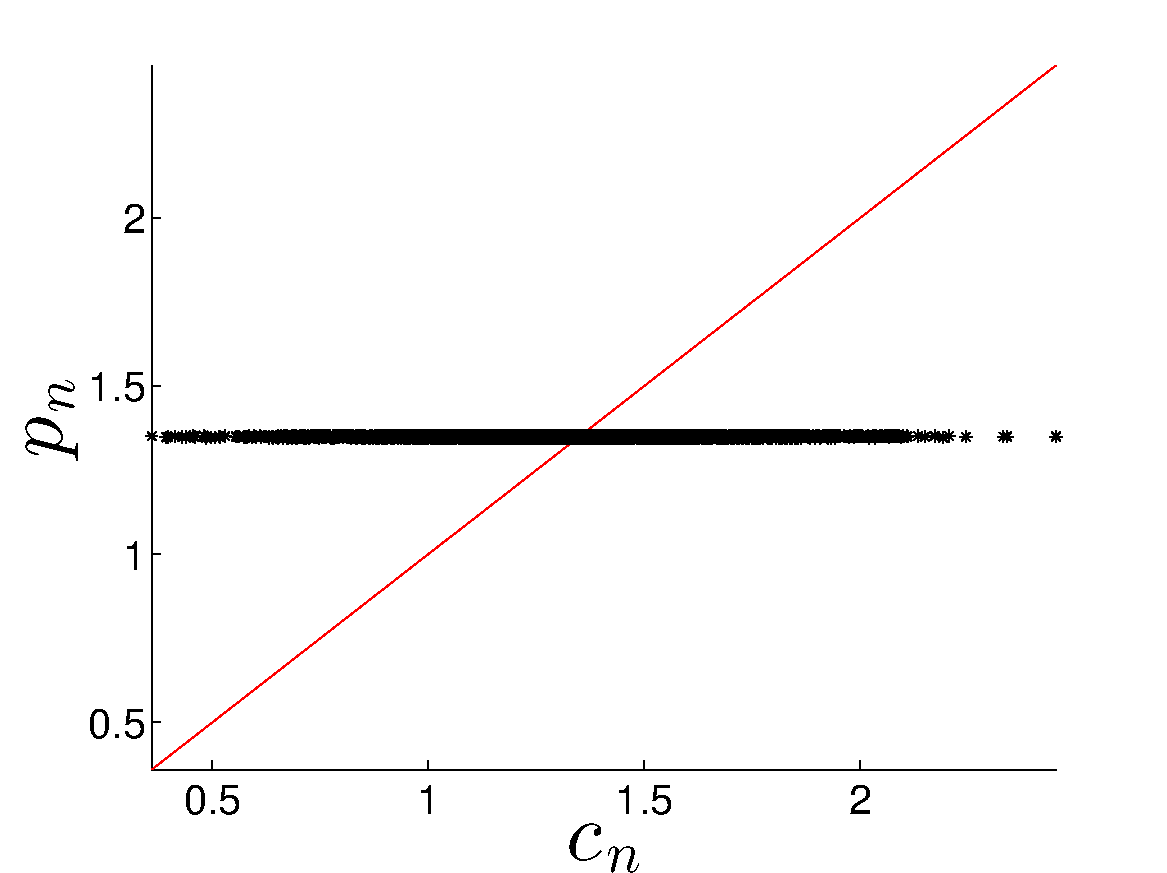
\includegraphics[width=0.6\columnwidth]{figs/gccMeanForecast} &
    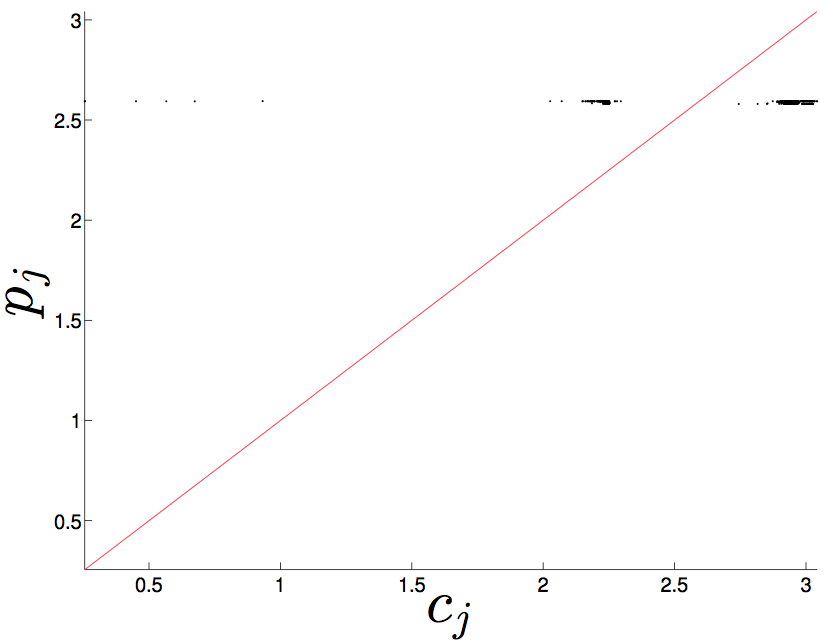
\includegraphics[width=0.6\columnwidth]{figs/svdfiveMeanForecast} \\
    \begin{sideways}\large ARIMA\end{sideways} &
    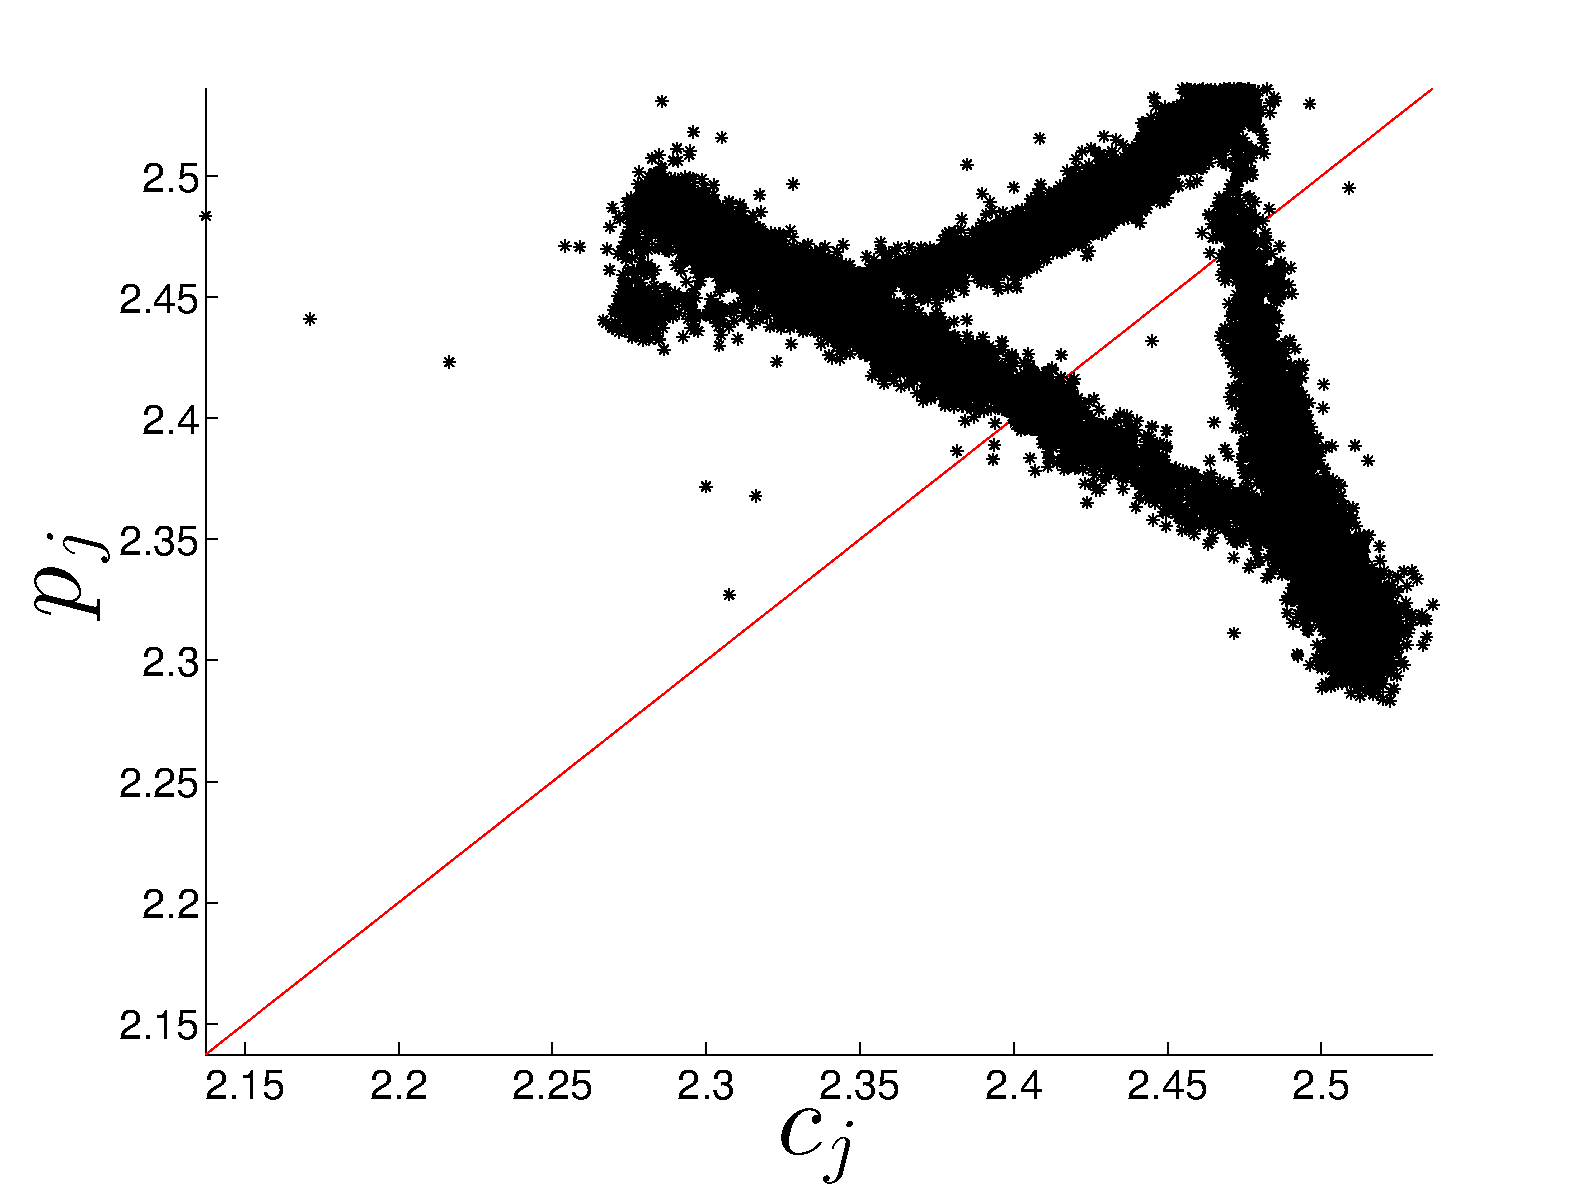
\includegraphics[width=0.6\columnwidth]{figs/colARIMAForecast} &
    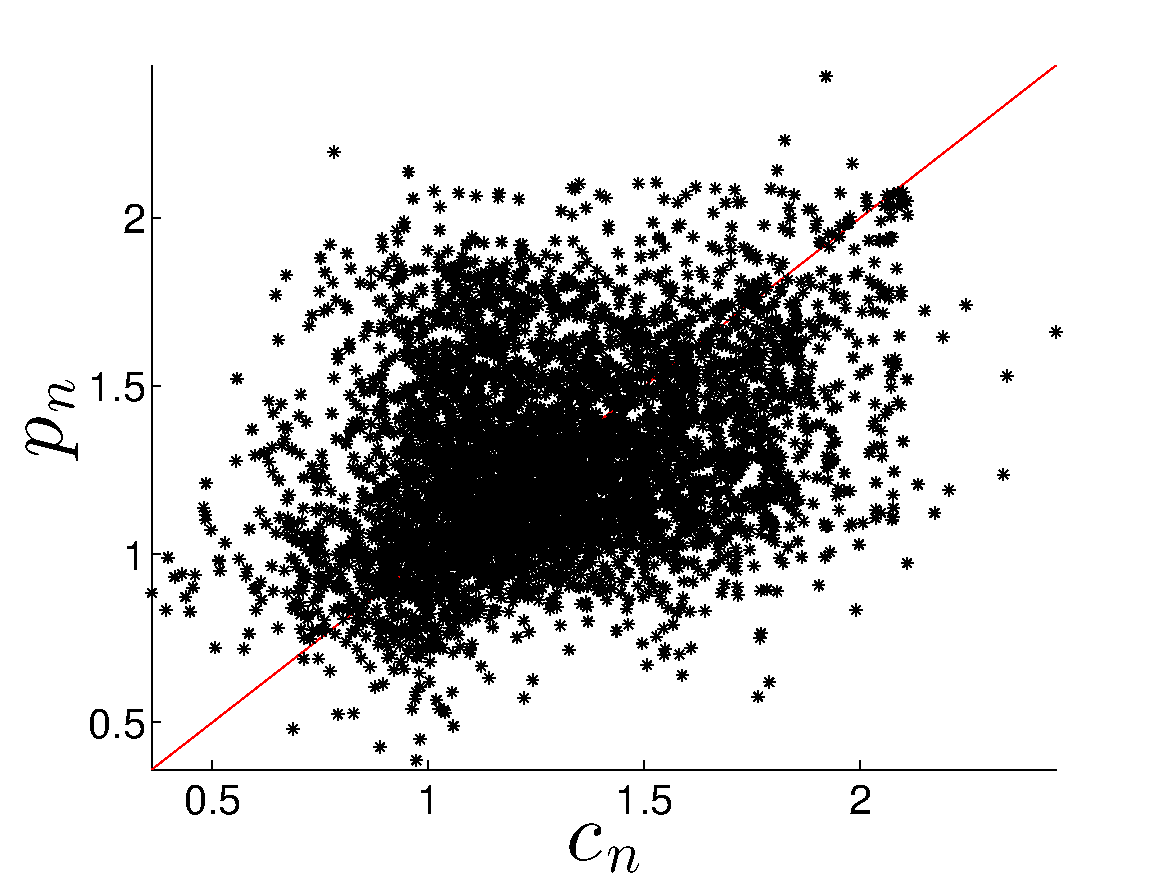
\includegraphics[width=0.6\columnwidth]{figs/gccARIMAForecast} &
    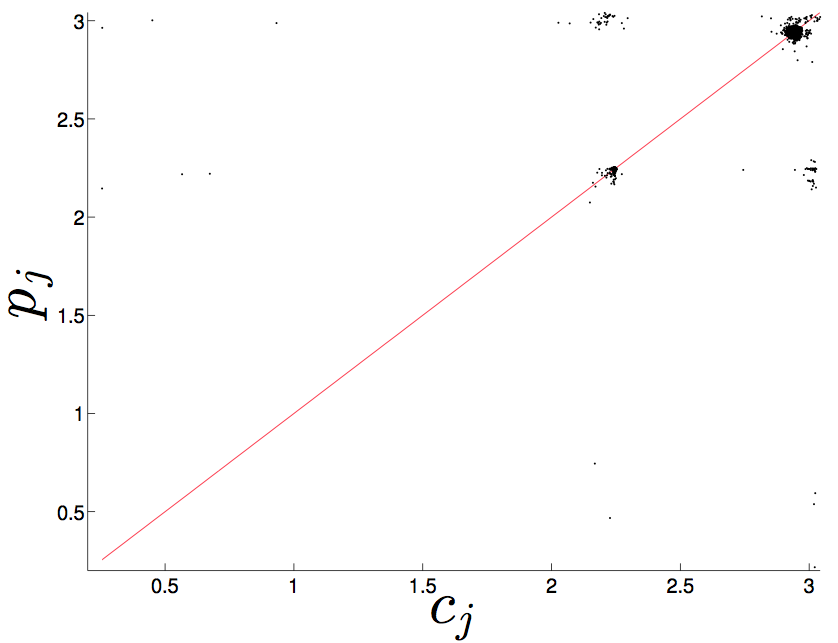
\includegraphics[width=0.6\columnwidth]{figs/svdfiveARIMAForecast} \\
    \begin{sideways}\large LMA\end{sideways} &
    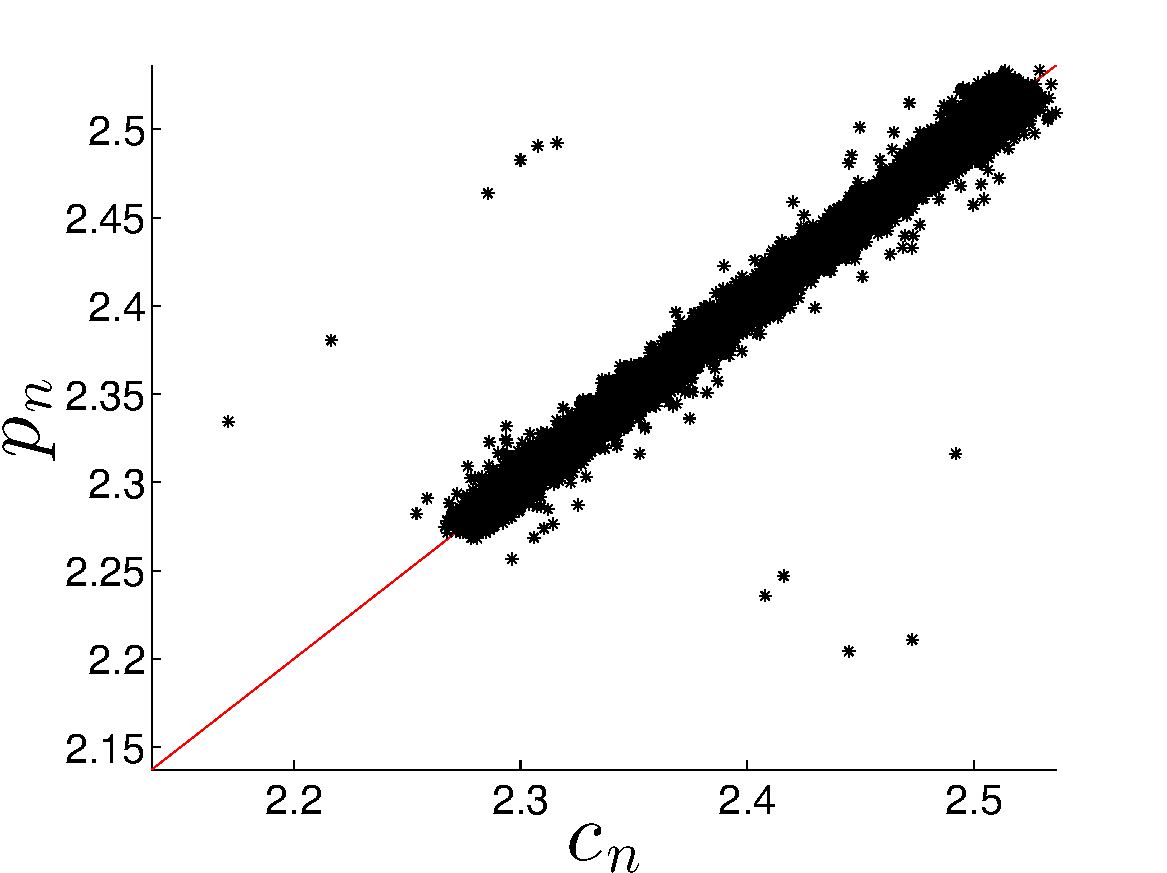
\includegraphics[width=0.6\columnwidth]{figs/colLMAForecast} &
    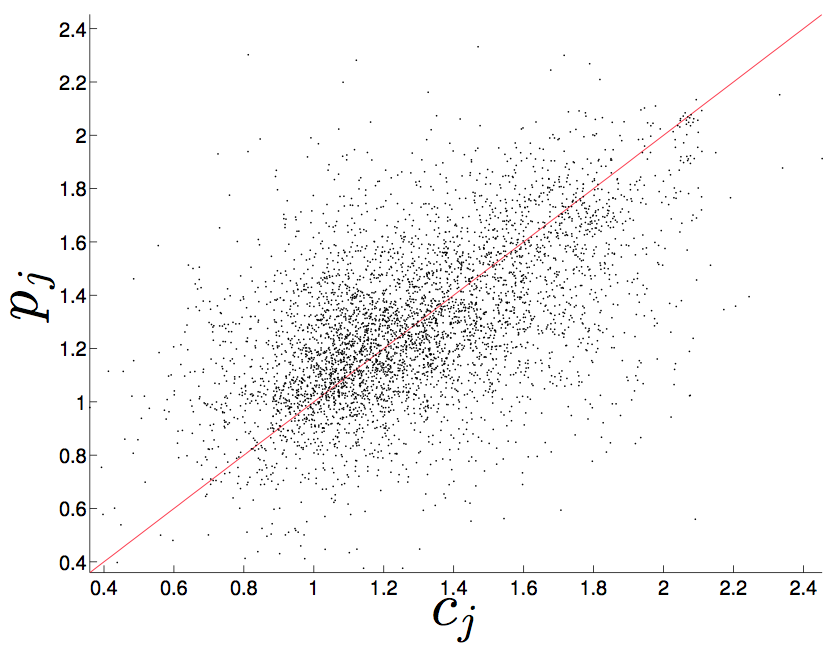
\includegraphics[width=0.6\columnwidth]{figs/gccLMAForecast} &
    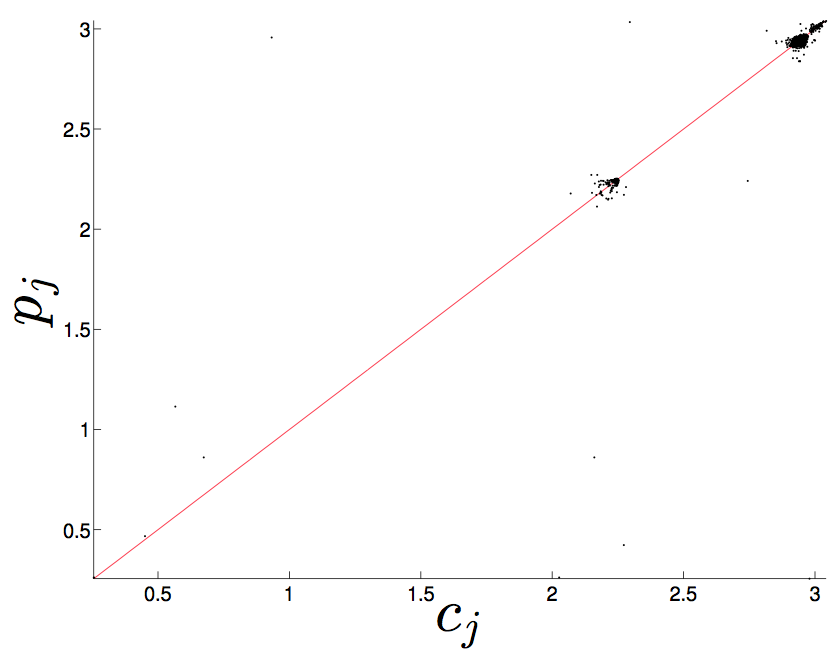
\includegraphics[width=0.6\columnwidth]{figs/svdfiveLMAForecast}
  \label{fig:forecast-example}
  \end{tabular}
  \caption{Predicted ($p_j$) versus true values ($c_j$) for forecasts of \col,
     \gcc, and \svdfive and all four prediction strategies.
  }
  \label{fig:forecast-example}
\end{table*}

In these images, the vertical axis is the prediction $p_j$ and the
horizontal axis is the true continuation $c_j$.  On such a plot, a
perfect prediction would lie on the diagonal.  LMA, for instance,
generates a very accurate prediction of the \col data, while ARIMA
does not.  Horizontal lines result when a constant predictor (e.g.,
\naive) is used on a non-constant signal.  Point clouds reflect the
structure of the distribution of the errors---roughly normally
distributed, for example, in the case of LMA on \gcc.  Note that the
shapes of Figures~\ref{fig:colRW} and~\ref{fig:colARIMA} are
reminiscent of the projected embedding in Figure~\ref{fig:embedding}a.
For a random-walk predictor, a $p_j$ vs. $c_j$ plot is equivalent to a
two-dimensional embedding with $\tau=1$.  For ARIMA, the
correspondence is not quite as simple, since the $p_j$ values are
linear combinations of a number of past values of the $c_j$, but the
effect is largely the same\footnote{The temporal \emph{ordering} of
  the points on the ARIMA $p_j$ vs. $c_j$ plot does not match that of
  a projected embedding of the time series, however.}.

As a numerical measure of prediction accurary, we calculate the mean
absolute scaled error (MASE) between the true and predicted signals:
%
$$MASE = \sum_{j=n+1}^{k+n+1}\frac{|p_j-c_j|
}{\frac{k}{n-1}\sum^n_{i=2}|x_{i}-x_{i-1}|}$$
%
This error metric was introduced in \cite{MASE} as a ``generally
applicable measurement of forecast accuracy without the problems seen
in the other measurements."  MASE is a normalized measure: the scaling
term in the denominator
%
% of the MASE value
% $$\frac{1}{n-1}\sum^n_{i=2}|X_{i,obs}-X_{i-1,obs}|$$
%
is the average in-sample forecast error for a random-walk prediction
over the initial training signal $\{x_i\}^n_{i=1}$.  That is, $MASE<1$ means that the
prediction error in question was, on the average, smaller than the
error of a random-walk forecast on the same data.  Analogously,
$MASE>1$ means that the corresponding prediction method did
\emph{worse}, on average, than the random-walk method.  We chose this
error metric because it allows for fair comparison across varying
methods, prediction horizons, and signal scales.

MASE scores for all 360 experiments are tabulated in the three
middle columns in Table~\ref{tab:error}.
\begin{table*}
\caption{Mean
absolute scaled error (MASE) scores and weighted permutation entropies for all eight
   processes studied in this paper}
  \begin{center}
  \begin{tabular*}{\textwidth}{@{\extracolsep{\fill} } ccccc}
  \hline\hline Signal & LMA MASE  & ARIMA MASE & na\"{i}ve MASE  & Weighted Permutation Entropy \\
  \hline
 \col           & $ 0.050 \pm0.002  $ & $0.599  \pm 0.211 $ & $0.571\pm0.002$&  $0.513 \pm 0.003$ \\

\gcc           & $ 1.530\pm 0.021$ & $1.837 \pm0.016 $ & $0.951 \pm 0.001$ & $0.943 \pm 0.001$ \\

\svdone     & $ 0.827\pm 0.076$ & $ 0.714\pm 0.075 $ & $2.676\pm4.328$&  $0.957 \pm 0.016$ \\

 \svdtwo    & $1.279 \pm0.020 $ & $2.163 \pm0.027 $ &  $3.054\pm0.040$ &   $0.846 \pm0.004$ \\

\svdthree     & $0.619 \pm0.021 $ & $0.713 \pm 0.010 $ & $31.386\pm 0.282$ &  $0.716 \pm 0.006$ \\
 \svdfour     & $ 0.779\pm0.036 $ & $0.979 \pm0.032 $ & $2.661\pm0.074$ & $0.825 \pm 0.008$ \\

\svdfive     & $ 0.718\pm 0.048 $ & $2.370  \pm 0.051 $ & $20.870 \pm 0.192$&  $0.678 \pm 0.007$ \\
 \svdsix     & $ 0.739\pm 0.068 $ & $ 1.438\pm 0.061$ & $2.197\pm0.083$&  $0.748 \pm 0.011$ \\
  \hline\hline
  \end{tabular*}
  \end{center}
 \label{default}
 \label{tab:error}
  \end{table*}%
Comparing these with the geometry of the plots in
Figure~\ref{fig:forecast-example}, one can see some obvious
correspondences.  The average LMA MASE score for the \col signals
was $0.050$, for instance, while ARIMA scored much worse ($0.599$).
That is, LMA performed roughly 20 times better on \col signals than a
random-walk predictor, while ARIMA only outperformed random walk by a
factor of 1.7.  This is in accordance with the visual appearance of
the corresponding images in Figure~\ref{fig:forecast-example}.  While
the correspondence between MASE score and the visual appearance of
these kinds of plots is clear cut in this case, that is not always so.
The plots of LMA predictions of \col and \svdfive both lie near the
diagonal, for instance, but the corresponding MASE scores were very
different: $0.050$ for \col and $0.718$ for \svdfive (resp., 20 and
1.4 times better than random-walk forecasts of the same signals).
This is a result of the normalization in the MASE score calculation.
Recall from Section~\ref{sec:simple} that the random-walk method
performs especially poorly on signals that oscillate rapidly.  \col
fits this description, so the random-walk error on this signal---the
denominator of the three MASE scores in the first row of the
Table---is pathologically high, which skews those scores down.
Random-walk prediction is very effective for the \svdfive signal, on
the other hand, so the denominator is small and the MASE scores are
skewed upwards.  Normalization is, as is often the case, a double-edged
sword.  Here, it facilitates comparisons across signals of different
types and lengths, but its particular pathologies must be taken into
account, as discussed at more length in Section~\ref{sec:results}.

% Table \ref{tab:error} provides the MASE distributions
% {\color{red}[[Joshua: Ryan, Is this the right word? we give mean $\pm$
%       std. dev but some have very skewed right tails]]} for each of
% the eight signals and three prediction strategies, these are averaged
% over 15 runs of each signal-method combination. For later comparison,
% Table \ref{tab:error} also has the complexity measure we introduce in
% Section \ref{sec:meaComplex}.

%[[and cherry pick a few examples of \gcc and \col to put in the text ]]


%---works quite well on the trace in Figure~%\ref{fig:ipc}, as%
%shown in Figure~\ref{fig:lmacol}.
%
%\begin{figure}
%   \centering
%\begin{subfigure}{\columnwidth}
%    \includegraphics[width=\columnwidth]{%colPredShortTS}
%    \caption{\col }
%    \label{fig:lmacol}
%  \end{subfigure}%
%
%    \begin{subfigure}{\columnwidth}
%    \includegraphics[width=\columnwidth]{%colPredShortTS}
%    \caption{\gcc}
%    \label{fig:lmagcc}
%  \end{subfigure}
%  \begin{subfigure}{\columnwidth}
%%    \includegraphics[width=\columnwidth]{%colPredShortTS}
%    \caption{\svdfive}
%    \label{fig:lmasvdfive}
%  \end{subfigure}%
%  \caption{{\color{red} [[If Liz thinks we should %include these I actually need to generate this %figure]]}An LMA-based forecast of
%       processor-efficiency performance trace from the%\col ,\gcc and \svdfive generating processes.  Red %circles and blue $\times$s are the true and
%       predicted values, respectively; vertical bars %show where these
%       values differ.}\label{fig:lmapredictions}
% \end{figure}
%
%\begin{figure}[htbp]
%  \centering
%   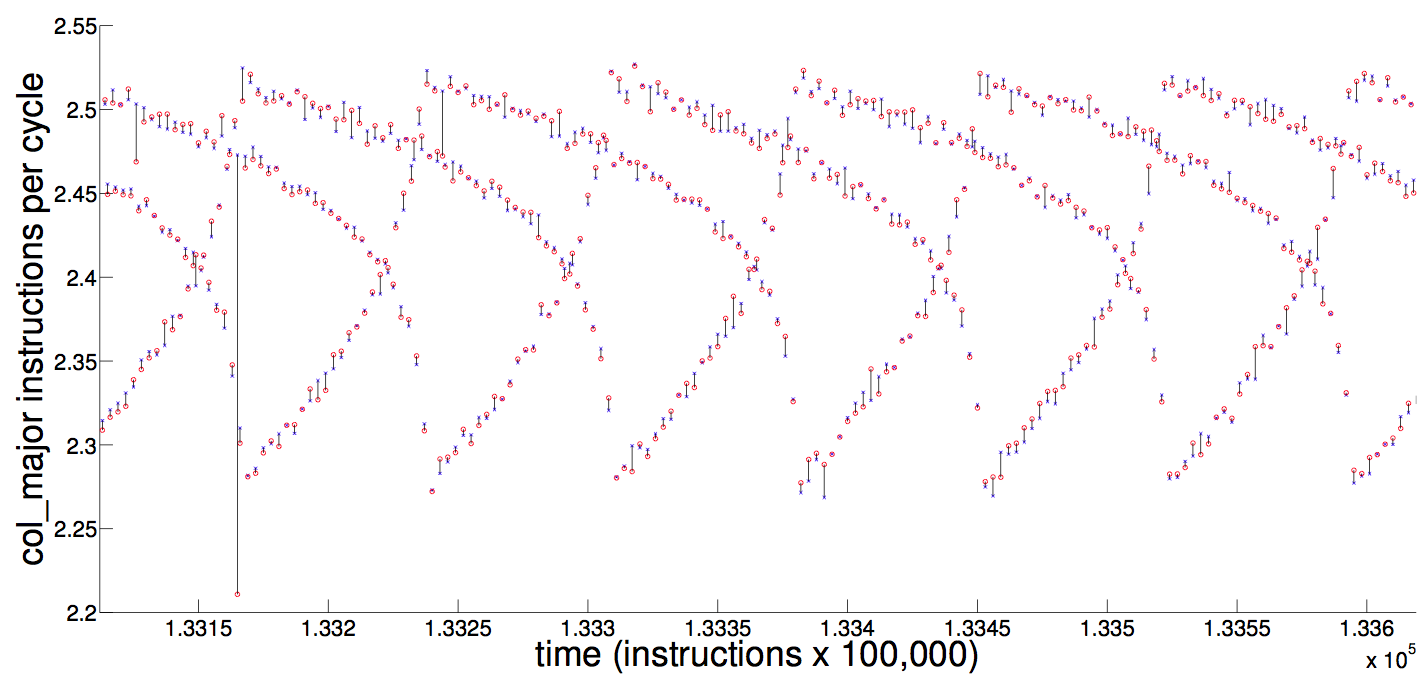
\includegraphics[width=\textwidth]{colPredShortTS}
%    \caption{A forecast of the last 4,000 points of the %signal in
%      Figure~\ref{fig:ipc} using an LMA-based strategy on %the
%      embedding in Figure~\ref{fig:embedding}.  Red circles %and blue
%      $\times$s are the true and predicted values, %respectively;
%      vertical bars show where these values differ.}
%\label{fig:lmacol}
%\end{figure}
%
%\begin{figure}[htbp]
%  \centering
%    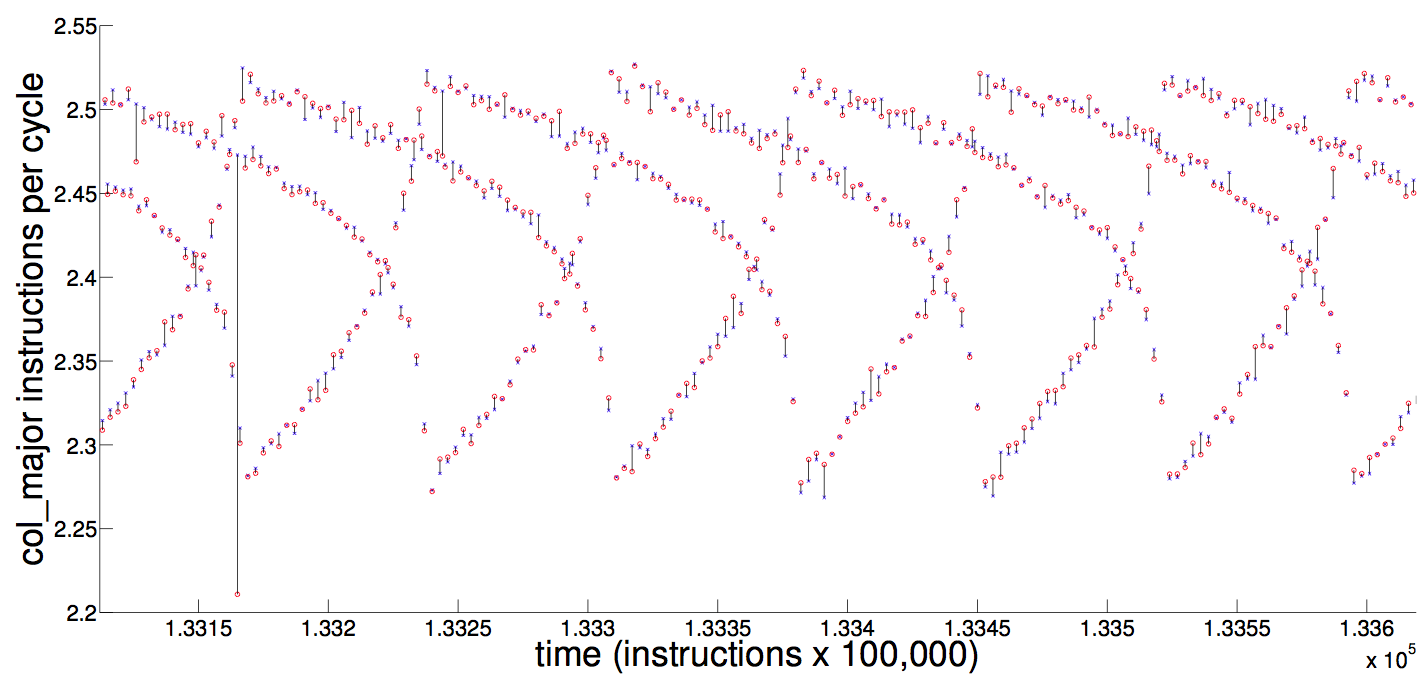
\includegraphics[width=\textwidth]{colPredShortTS}
%     \caption{{\color{red} [[actually need to generate this %figure]]}An LMA-based forecast of the last 4,000 points of a
%       processor-load performance trace from the \gcc
%       benchmark.  Red circles and blue $\times$s are the %true and
%       predicted values, respectively; vertical bars show %where these
%       values differ.}
%\label{fig:lmagcc}
%\end{figure}
%
%On the other hand, if we use the same approach to %forecast the
%processor efficiency (IPC) of the \gcc time series, %the
%prediction is far less accurate; see Figure~%\ref{fig:lmagcc}.
%Figure~\ref{fig:lmasvdfive} is clearly a better %prediction than Figure~\ref{fig:gccLMA} but not nearly as good as the \col forecast.


%This gets at the utility of the contribution of this %paper: These time series all come from the same system---computers---but they are not equally predictable (at this point by LMA). For a practitioner is it the case that
%  Our
%conjecture is that while they come from similar systems \gcc produces processor load traces on the top of the complexity spectrum whereas \col produces processor loads with complexity in the mid to low region of the complexity spectrum. If this is the case then \gcc might be much better predicted using a method like Random Walk or \naive which can effectively predict in the presence of complexity. This is explored more rigorously in the results Section of this paper (Section \ref{sec:results}. So that we don't have to compare the forecast accuarcy by visual comparing the predictions we calculate a figure of merit to compare the predictions.






\section{Measuring Structural Complexity }\label{sec:meaComplex}

The goal of the section is to describe our solution to the challenging
problem of estimating the entropy of an arbitrary, real-valued time
series.  This approach draws upon methods and results from a variety
of fields including time-series analysis, dynamical systems, and
stochastic processes.

For the purposes of this paper, we view the Shannon entropy---in
particular its growth rate with respect to word length (the
\emph{Shannon entropy rate})---as a measure of complexity and
unpredictability in a time series.  A time series with a high entropy
rate is almost completely unpredictable; conversely one with low
entropy rate is often quite predictable. {\color{red} [[does the claim
      in the previous sentence need a citation, a justification, or an
      ``in practice,''?]]}  This can be made more rigorous: Pesin's
relation \cite{pesin77} states that in chaotic dynamical systems, the
Kolmogorov-Sinai (KS) entropy is equal to the sum of the positive
Lyapunov exponents, $\lambda_i$.  The Lyapunov exponents directly
quantify the rate at which nearby states of the system diverge with
time: $\left| \Delta x(t) \right| \approx e^{\lambda t} \left| \Delta
x(0) \right|$.  The faster the divergence, the larger the entropy, and
the more difficult prediction becomes.  The KS entropy is defined as
the supremum of the Shannon entropy rates of all
partitions~\cite{petersen1989}. The partition that achieves this
supremum is the \emph{generating partition} discussed in
Section~\ref{sec:related}.

From a different point of view, we can consider the information (as
measured by the Shannon entropy) contained in a single observable, say
the \emph{present}, of the system. This information can be partitioned
into two components: the information shared with past
observations---e.g., the mutual information between the past and
present---and the information in the present that is not contained in
the past (aka ``the conditional entropy of the present given the
past'').  The first part is known as the \emph{redundancy}, as it is
information in the present which is also in the past.  The second part
is the aforementioned \emph{Shannon entropy rate}.  In theory, the
more redundancy in a signal, the more predictable it is {\color{red}
  [[citation for that theory?]]}.  Redundancy is critical to
prediction, in general.  And the specific \emph{form} of the
redundancy dictates whether a particular prediction method will work
well or poorly on the corresponding signal.  A linear method cannot
detect or make use of nonlinear redundancy, for instance.  This issue
is central to the claims in this paper and the discussion in the
following section.

Utilizing Shannon entropy rate as a measure of temporal complexity is
not a new idea \cite{Shannon1951, mantegna1994linguistic}, but
previous approaches required categorical data: $x_t \in \mathcal{S}$
for some finite or countably infinite \emph{alphabet} $\mathcal{S}$.
Data taken from real-world systems is, however,
effectively\footnote{Measurements from finite-precision sensors are
  discrete, but data from modern high-resolution sensors are, for the
  purposes of entropy calculations, effectively continuous.}
real-valued.  To analyze real-valued data using a method that requires
categorical values, one must discretize the data---typically by
binning.  Unfortunately, this is rarely a good solution, as the
binning of the values introduces spurious dynamics~\cite{bollt2001}.
The field of symbolic dynamics offers discretization methods that do
not disturb the intrinsic behavior.  These methods are, however,
fragile in the face of noise; worse yet, they require knowledge of the
underlying system.  This is not useful in our context, where we want
to measure the entropy to quantify predictability.

Bandt and Pompe introduced the \emph{permutation entropy} (PE) as a
``natural complexity measure for time series''
\cite{bandt2002per}. Permutation entropy employs a method of
discretizing real-valued time series that follows the intrinsic
behavior of the system under examination.  Rather than looking at the
statistics of sequences of values, as is done when computing the
Shannon entropy, permutation entropy looks at the statistics of the
\emph{orderings} of sequences of values using ordinal
analysis. Ordinal analysis of a time series is the process of mapping
successive time-ordered elements of a time series to their
value-ordered permutation of the same size.  By way of example, if
$(x_1, x_2, x_3) = (9, 1, 7)$ then its \emph{ordinal pattern},
$\phi(x_1, x_2, x_3)$, is $231$ since $x_2 \leq x_3 \leq x_1$.  The
ordinal pattern of the permutation $(x_1, x_2, x_3) = (9, 7, 1)$ is
$321$.  {\color{red} [[This method has many features; among other
      things, it is generally robust to observational noise and
      requires no knowledge of the underlying mechanisms.]] [[This
      sentence is out of place.]]}

\begin{mydef}[Permutation Entropy]

  Given a time series $\{x_t\}_{t = 1,\dots,T}$. Define $\mathcal{S}_\ell$ as all $\ell!$ permutations $\pi$ of order $\ell$. For each $\pi \in \mathcal{S}_\ell$ we determine the relative frequency of that permutation occurring in $\{x_t\}_{t = 1,\dots,T}$:
  \begin{align*}
    P(\pi) = \frac{\left|\{t|t \leq T-\ell,\phi(x_{t+1},\dots,x_{t+\ell}) = \pi\}\right|}{T-\ell+1}
  \end{align*}
  where $P(\pi)$ quantifies the probability of an ordinal and
  $|\cdot|$ is set cardinality. The \emph{permutation entropy} of
  order $\ell \ge 2$ is defined as
  \begin{align*}
    H(\ell) = - \sum_{\pi \in \mathcal{S}_\ell} P(\pi) \log_2 P(\pi)
  \end{align*}

\end{mydef}

Notice that $0\le H(\ell) \le \log_2(\ell!)$ \cite{bandt2002per}.
With this in mind, it is common in the literature to normalize
permutation entropy as follows: $\frac{H(\ell)}{\log_2(\ell!)}$.  With
this convention, ``low'' PE is close to 0 and ``high'' PE is close to
1. Finally, it should be noted that the permutation entropy has been
shown to be identical to the Kolmolgorov-Sinai entropy for many large
classes of systems \cite{amigo2012permutation}, so long as
observational noise is sufficiently small. As mentioned before, this
is equal to the Shannon entropy rate of a generating partition of the
system.  {\color{red} [[What this normalization allows us to do, then,
      is approximate the redundancy of a signal by $1 -
      \frac{H(\ell)}{\log_2(\ell!)}$.]] [[This sentence is out of
      place.  Shouldn't it be before the sentence that starts with
      ``Finally...''?]]}

Here we will be utilizing a variation of the basic permutation entropy
technique, the \emph{weighted permutation entropy} (WPE), which was
introduced in~\cite{fadlallah2013}.  The intent behind the weighting
is to correct for observational noise that is larger than the trends
in the data, but smaller than the larger scale features.  Consider,
for example, a signal that switches between two fixed points and
contains some additive noise.  {\color{red} The weighted permutation
  entropy would be dominated by the switching rather than by the
  stochastic fluctuation. To accomplish this, [[I am completely
      confused by the wording here.  Do you mean that the {\bf
        original} PE would be dominated?  And that you don't want
      that?  If not, you need to fix this wording -- i.e., ``would''
      to ``should'' and an explanation of why one would want to
      calculate a PE that captures the switching.]]} the \emph{weight}
of a permutation is taken into account:
\begin{align*}
  w(x_{t+1:t+\ell}) = \frac{1}{\ell} \sum_{x_i \in \{x_{t+1:t+\ell}\}}
                      \left( x_i - \bar{x}_{t+1:t+\ell} \right)^2
\end{align*}
where $x_{t+1:t+\ell}$ is a sequence of values $x_{t+1}, \ldots,
x_{t+\ell}$, and $\bar{x}_{t+1:t+\ell}$ is the arithmetic mean of
those values.

The weighted probability of a permutation is then:
\begin{align*}
  P_w(\pi) = \frac{\displaystyle \sum_{t \le T - \ell} w(x_{t+1:t+\ell}) \cdot \delta(\phi(x_{t:t+\ell}), \pi) }{\displaystyle \sum_{t \le T - \ell} w(x_{t+1:t+\ell})}
\end{align*}
where $\delta(x, y)$ is 1 if $x = y$ and 0 otherwise. Effectively,
this weighted probability enhances permutations that are involved in
``large'' features and de-emphasizes permutations that are small in
amplitude relative to the features of the time series.  {\color{red}
  [[The weighted permutation entropy is then:]] [[you used exactly
      these words above.  what is the textual causality of this
      ``then'' and that ``then''?]]}
\begin{align*}
  H_w(\ell) = - \sum_{\pi \in \mathcal{S}_\ell} P_w(\pi) \log_2 P_w(\pi),
\end{align*}
which can also be normalized {\color{red} [[why?]]}  by dividing by
$\log_2(\ell!)$.  This normalization is used in all the results that
follow.

In practice, calculating permutation entropy and weighted permutation
entropy involves choosing a good value for the word length $\ell$. The
primary consideration here is that the value be large enough that
forbidden ordinals are discovered, yet small enough that reasonable
statistics over the {\color{red} [[existing??]]}  ordinals are
gathered.  If an average of 100 counts per ordinal is considered to be
sufficient, for instance, then $\ell =
\operatornamewithlimits{argmax}_n \{ T \gtrapprox 100 n! \}$.  In the
literature, $3 \le \ell \le 6$ is a standard choice---generally
without any formal justification.  In theory, the permutation entropy
should reach an asymptote with increasing $\ell$, but that can require
an arbitrarily long time series. In practice, what one should do is
calculate the \emph{persistent} permutation entropy by increasing
$\ell$ until the result converges, but data length issues can intrude
before that convergence is reached.  We used this approach to choose
$\ell = 6$ for the experiments in the following section.  This value
represents a good balance between accurate ordinal statistics and
finite-data effects.

As a final note: there has been prior work under a similar title to
ours~\cite{haven}, but there are only superficial similarities between
the two research projects.  Haven {\sl et al.} utilize the relative
entropy to study how well small ensembles predict the distribution of
future states of dynamical (and potentially chaotic) systems.  Our
work quantifies the predictability of a single observed time series
using weighted permutation entropy and makes no assumptions about the
underlying dynamics.  {\color{red}[[Why is WPE better than relative
      entropy?]]}.

% was a good choice, because with $\ell \geq 7$ many signals had
% entropies plummet due to finite data effects and so with a word length
% of 6 we are capturing as much structure as possible without
% sacraficing the accuracy of ordinal statistics.

%\subsection{Regime Selection:Detecting complexity shift in a time series}\label{sec:wpeRegime}
%
%{\color{red} this is from a previous paper I wrote, if this is used we need to update the plots to use wpe and windowed wpe instead of standard pe, also not sure how much of this is necessary but added as starting point}
%
%Permutation entropy is a measure of the complexity of time series as a whole, but it can also be used to calculate a dynamical shift in a time series as illustrated in \cite{cao2004det}. To detect dynamical changes in a time series we follow the methods of \cite{cao2004det}. Partition the time series  $\{x_t\}_{t = 1,\dots,T}$ into overlapping\footnote{Following \cite{cao2004det} we use maximal overlapping block. (A window shift of 1.)} (or nonoverlapping) blocks. Calculate $H(n)$ for each block, and treat $H(n)$ as a function of time.  According to \cite{cao2004det} drastic changes in permutation entropy can indicate change in the underlying model.
%
%In addition to introducing this block method, \cite{cao2004det} introduce the use of a \emph{lag} when calculating permutation entropy. This is identical to the lag used in delay coordinate embedding and often the same language is used. Cao et al. describe the process of symbolization in \cite{bandt2002per} as embedding the time series in an $m$ dimensional symbol space. When we symbolize a scalar time series,$\{x_t\}_{t = 1,\dots,T}$, we first embed the scalar time series into $m$ dimensional vectors before matching this to a symbol in $\mathcal{S}_m$. So pre-symbolization our time series changes from scalar to objects of the form:  $$[x(i),\,x(i+1),\,\dots,x(i+(m-1)]$$ This vector is then mapped by $\phi$ to a symbol in $\mathcal{S}_m$. Cao et al. argue that we can view this as embedding the time series in an $m$ dimensional space with lag 1. Cao et al. then state ``Since in practice the optimal $L$[lag] may be different from 1, we shall present the idea for any $m$[embedding dimension] and $L$."\footnote{No further explanation is given about why this is the case.} To not confuse notation we define $\tau$ to be the lag parameter. The process of symbolization then starts with transforming the scalar time series into a set of vectors of the form $$[x(i),\,x(i+\tau),\,\dots,x(i+(m-1)\tau]$$ where $\tau\ge1$.
%
%\subsubsection{Example: Concatenated Time Series}\label{sec:concatenate}
%As an example of this detection, consider Figure \ref{fig:ts-banded} (a). This is a plot of a concatenated time series comprised of several orbits of the Logistic map with varying parameters as well as intermittent noise. Each concatenated band (either an orbit of the Logistic map or noise) is 50,000 points. The bands of noise are generated with Matlab's \verb|randsample|, using the chaotic bands as the sampling population. Each Logistic map trajectory begins at $x=0.6$. The period-two trajectories have an $R$ of 3.2, the period-three trajectory has an R of 3.838, and the chaotic trajectories have an $R$ of 3.65.
%
%The concatenated time series is comprised of two period-two trajectories($t=0-50,000$ and $t=250,000-300,000$), one period-three trajectory($t=100,000-150,000$), two chaotic trajectories ($t=50,000-100,000$ and $t=200,000-250,000$, and two different bands of noise($t=150,000-200,000$ and $t=300,000-350,000$). Visually the bands of noise and the chaotic trajectory are indistinguishable. If this were an observed time series from a real process, it would be impossible to visually identify which bands were generated deterministically and which were simply noise. If we calculate block permutation entropy as discussed in \cite{cao2004det} and plot this as a function of time it becomes very clear which bands have structure and which do not.
%
%In Figure \ref{fig:ts-banded} (b) we plot the concatenated time series, as well as permutation entropy as a function of time(red, blue and green curves). The red, blue and green curves are the permutation entropy calculated using $m=5$ and $\tau = 1,2,3$ (respectively). Using these curves it is clear that bands 2 and 5 ($t=50,000-100,000$ and $t=200,000-250,000$) are chaotic because they have structure\footnote{Permutation entropy less than one.}. On the other hand, bands 4 and 7 ($t=150,000-200,000$ and $t=300,000-350,000$) have no structure\footnote{Permutation entropy of one.} and are the noise bands. This is in fact the case when comparing to the way the time series was constructed.
%
%The main advantage we can see to the use of lags other than 1 is for analysis of periodicity. This is also the major advantage listed in \cite{cao2004det}. Notice in the period 2 bands the blue curve (permutation entropy calculated with a lag of 2) is zero. This means that with a lag of 2 the period 2 orbit is perfectly structured\footnote{Equivalently, not enough permutations are being realized to impact the calculation of $H(n)$}. If we increase the lag to 3 (the green curve) the two period-two bands have a little bit of structure(as some permutations will be realized) but the period 3 band has zero permutation entropy.
%
%%TSLogistic = [period2Logistic;chaosLogistic;period3Logistic;randomSampleFromMap2;chaosLogistic;period2Logistic;randomSampleFromMap3];
%
%%\begin{figure}
%%  \centering
%%  \subfigure{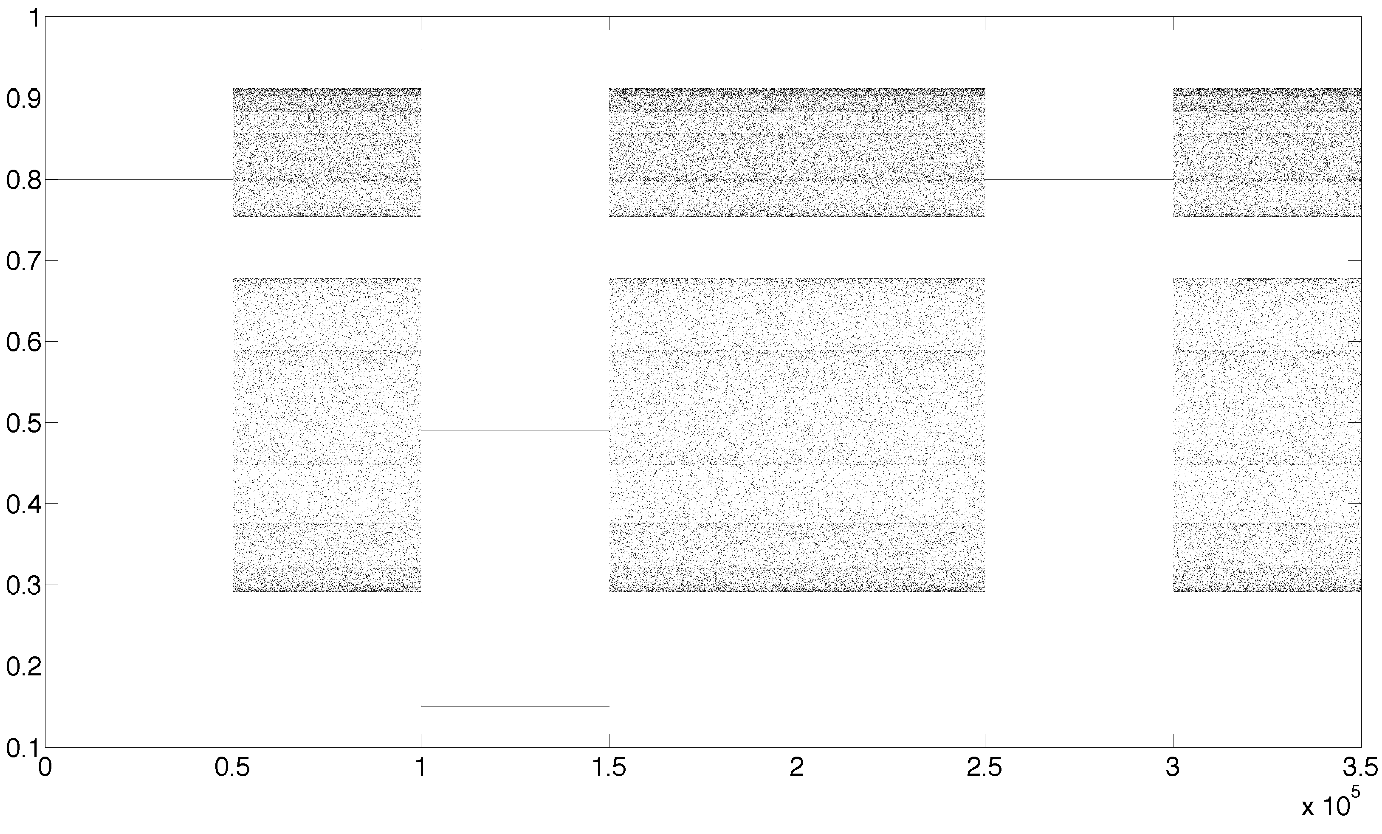
\includegraphics[width=\columnwidth]{unused-figs/ts-banded-alone}}
%%    {(a)}
%%
%%  \subfigure{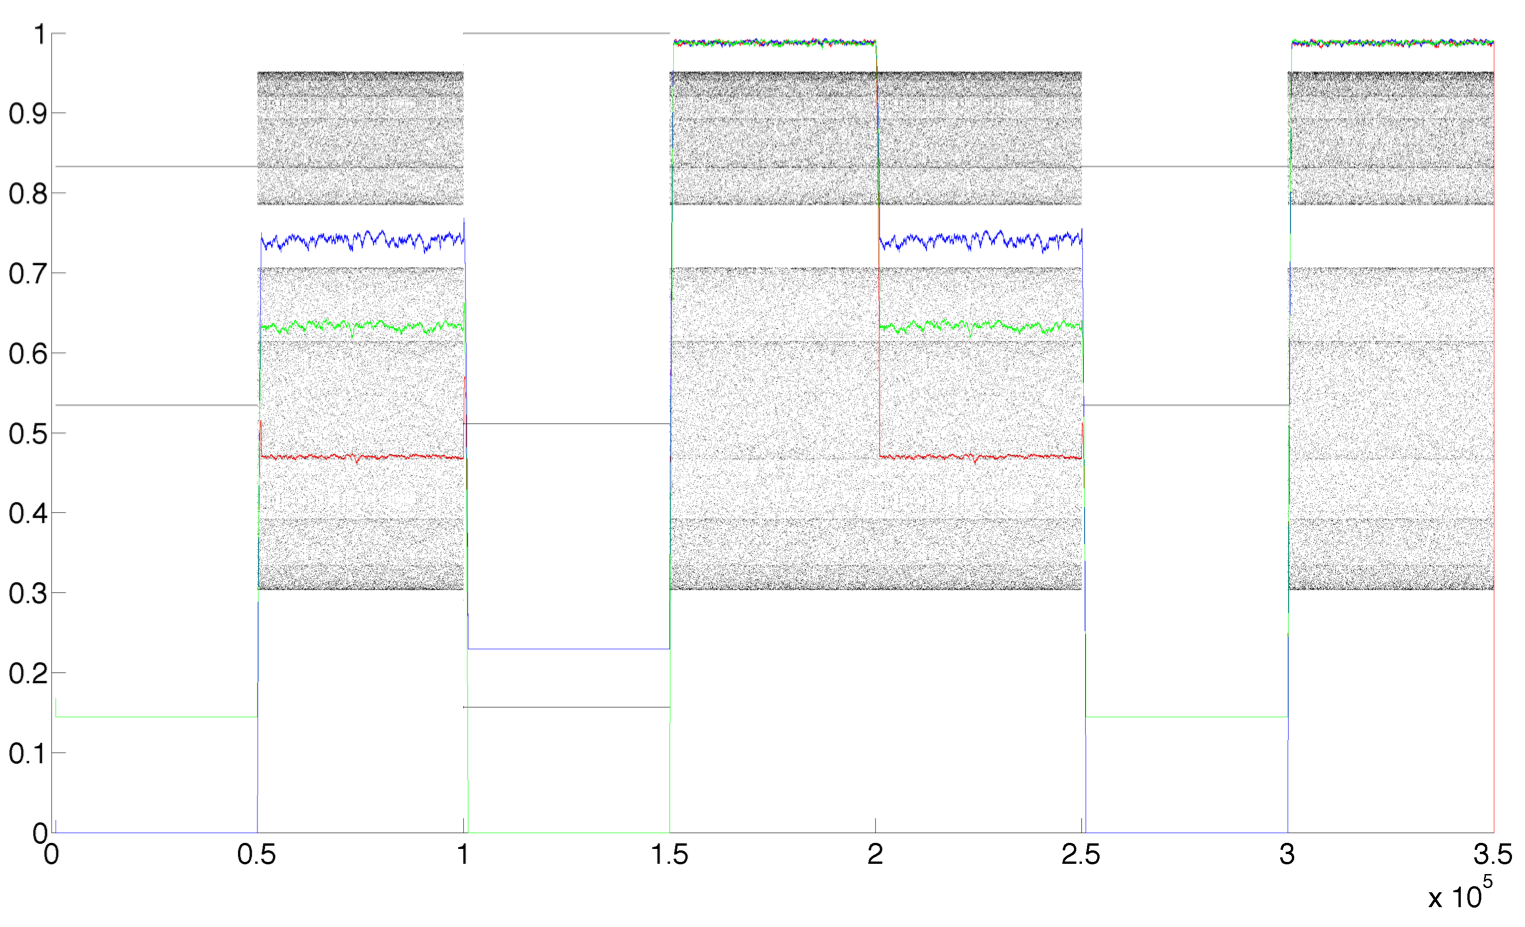
\includegraphics[width=\columnwidth]{unused-figs/ts-banded-pe}}
%%  {(b)}
%%  \caption{ (a) The concatenated time series discussed in Section~\ref{sec:concatenate}. (b) Plot of the concatenated time series from Section~\ref{sec:concatenate}, as well as permutation entropy as a function of time(blue,green and red curves). Each permutation entropy curve shown is calculated using $m=5$, however, the red,blue and green curve use a $\tau = 1,2,3$ respectively.}\label{fig:ts-banded}
%%\end{figure}
%
%
%
%
%
%
%and what is it good for with forward pointer to the other sections
%
%
%
%\subsubsection{Example: The transient Logistic map}
%In Section~\ref{sec:concatenate} we discussed a time series which stayed in a parameter regime for long amounts of time and then abruptly changed. As we showed, permutation was a great proxy to detect this change. Another type of parameter change that may occur in a physical system is constant parameter drift, i.e., some parameter slowly changes over time. To explore this type of parameter drift we construct the same time series as was used in \cite{cao2004det}. Iterate the logistic map, starting with $R=2.8$, then at every iteration increase $R$ by $10^{-5}$ until $R=4$. The time series, which can be seen in Figure~\ref{fig:translogistic} appears very similar to the standard bifurcation diagram for the Logistic map. The curves in red and blue are the permutation entropy calculated with $m=5$ and $\tau = 1,2$ (respectively).
%
% As we can see, as bifurcations occur in the dynamics the permutation entropy changes as well. An interesting feature of block calculations are the spikes that occur at bifurcation points. As the block begins to encompass multiple regimes, e.g., fixed point and  period two, permutations are being realized for both regimes. This overlap causes an increase in the time series complexity, and thus a spike in the permutation entropy. The dips you see in the second half correspond to bands of periodicity which occur between the chaos. It is worth noting, that the blue curve (permutation entropy with lag 2) does not go to zero in the period 2 parameter range. This is because this is not a true period 2 orbit but transient that is moving across \emph{several} period 2 orbits, thus it maintains a higher level of complexity, albeit still very low.
%
% This illustrates that permutation entropy can not only distinguish between instant (and drastic) parameter shifts but also very slow and gradual parameter drift.
%
%\begin{figure}[ht]
%  \centering
%  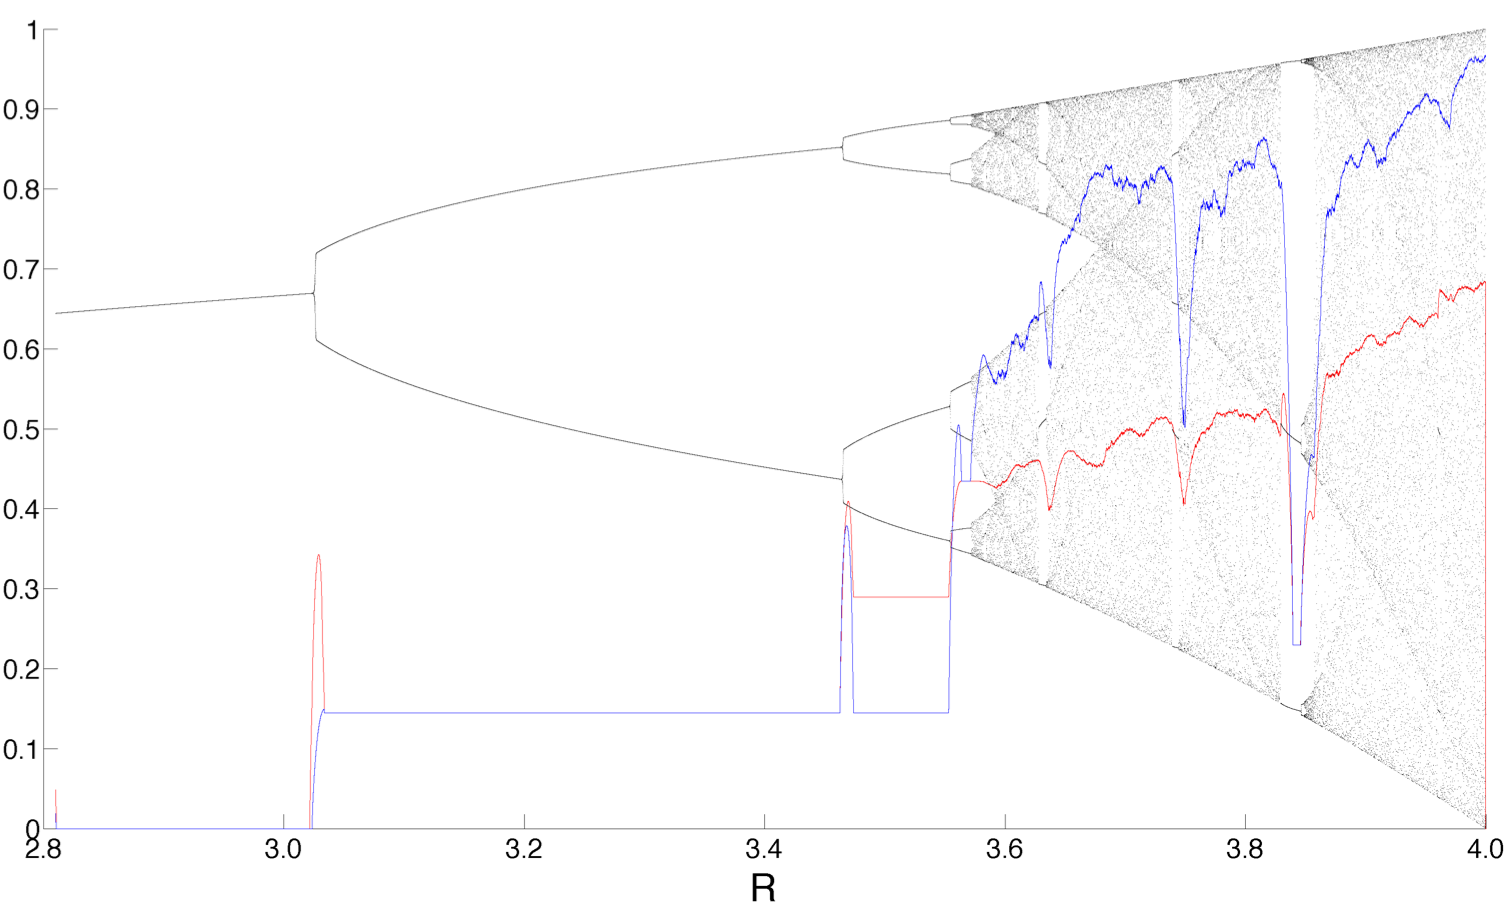
\includegraphics[width=\columnwidth]{unused-figs/tstranslog-perm}
%  \caption{Transient Logistic map time series and permutation entropy curves. Both permutation entropy curves are calculated with $m=5$, the red and blue correspond to $\tau = 1,2$ respectively.}
%  \label{fig:translogistic}
%\end{figure}
%%\begin{enumerate}
%%\item do with henon bifurcation. what happens near the broken chaotic window
%
%%\end{enumerate}
%
%
%The weighted permutation entropy for the \svd program is given in
%Fig.~\ref{fig:wwpe}. To generate this image a window of 5,000 values slid over
%the time series. Within each of those windows, the statistics over words of
%length 4 are computed and the WPE is calculated. The gray bands denote regions
%where the 5,000 value window overlapped visually-distinct regimes. It can be
%seen that the behaviors of the weighted permutation entropy vary between
%regimes. [[I think here it would be good to add a paragraph explaining the windowed WPE was used for regime choices on SVD...emphasizing  that over a time series permutation entropy fluctuates illustrating within a single time series different levels of complexity and predictability exist. Maybe point at some of the predicting predictability papers.]]
%
%%\begin{figure}[htbp]
%%  \centering
%%  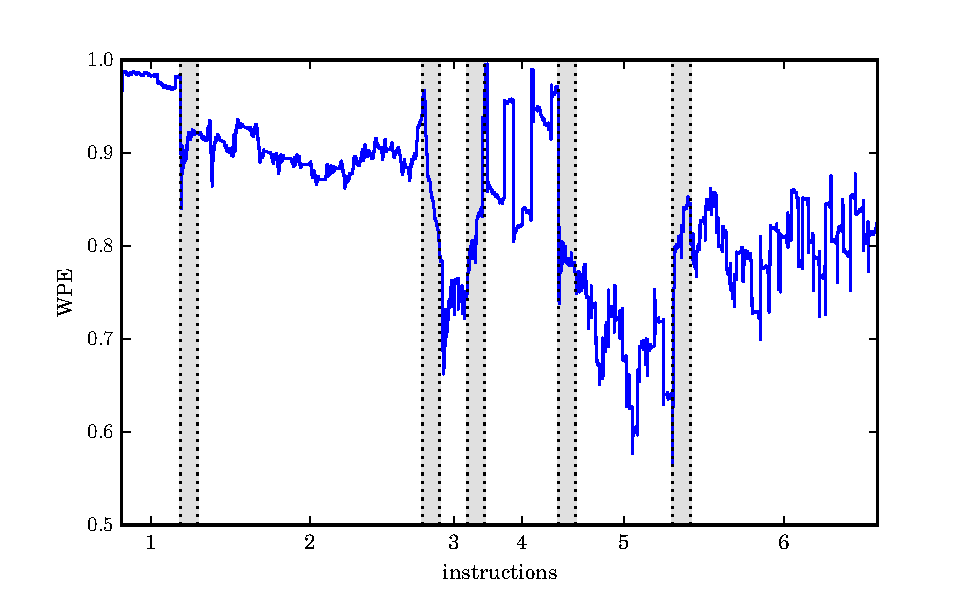
\includegraphics[width=1.0\textwidth]{figs/SVD_wwpe}
%%  \caption{[[Joshua: I think adding the colored SVD trace to this would be %good or putting it above this figure]]The weighted permutation entropy of %one run of SVD. The gray bands
%%    are regions where the window overlaps regimes. The window size used is
%%    $5,000 \times 100,000$ instructions and the word length is $4$.}
%%  \label{fig:wwpe}
%%\end{figure}
%
%
%%%FIGURE INTENT
%%This figure shows that entropy changs over time with the signal as well as why the regimes for \svd were chosen. 
%%%%%%%%%%%%%%%%%%
%\begin{figure}[htbp]
%  \centering
%  %\begin{subfigure}{0.3\textwidth}
%  %  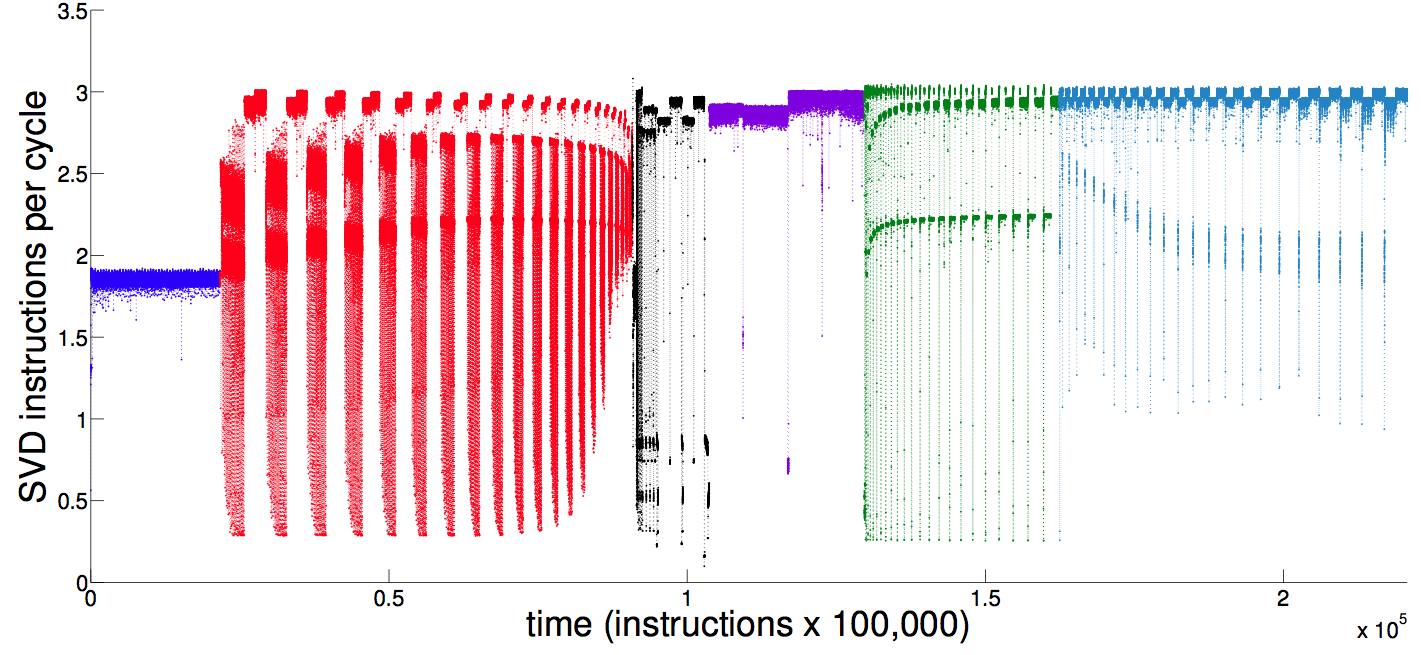
\includegraphics[width=0.3\textwidth]{figs/svdipcregimescolored.png}
%  %  \caption{The instructions per cycle of \svd. Each color corresonds to the different regimes as selected by rapid shifts in WPE, as seen in Figure \ref{fig:svd_wwpe}. From left to right each change in color represents a change in regime for 6 regimes in total. }
% %   \label{fig:svd_ts}
% % \end{subfigure}%
%  %\\
% % \begin{subfigure}{\textwidth}
%
% {\color{red}TODO: Put this image back in.}
%%Liz commented this image out temporarily so that her mac doesn't hang
%%when she scrolls past p12
%% We decided to skip the figure completely, since we took out
%% all stuff about PE as regime-shift detection.  
%% [[should add that as future work, though.]]
%  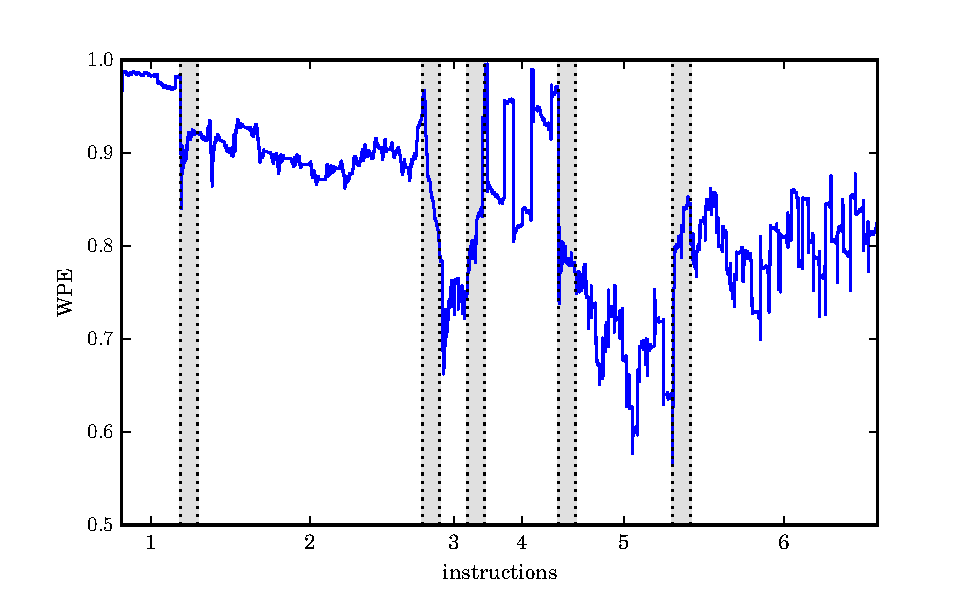
\includegraphics[width=\columnwidth]{figs/SVD_wwpe}
%  \caption{The weighted permutation entropy of one run of SVD. The gray bands are regions where the window overlaps regimes. The window size used is 5,000 $\times$ 100,000 instructions and the word length is $6$. For reference the instructions per cycle of \svd are plotted as a ghost behind this plot. Each color on the ghosted time series corresonds to the different regimes as determined by visual inspection. From left to right each change in color represents a change in regime for 6 regimes in total.}\label{fig:wwpe}
%\end{figure}
%





 \section{Predictability, Complexity, and Permutation Entropy %{\color{blue}  EDITABLE}
 } % (fold)
 \label{sec:results}
% I changed the title of this section because there are lots of
% results in the modeling section too.  The results HERE are about the
% relationship between predictability and WPE


%OUTLINE:
%\begin{enumerate}
%\item \cmark~Introduce MASE.
%\item \cmark~WPE is a good measure of predictability.  %Figure: best athlete MASE vs.
%its WPE.
%\item \cmark~Talk about structure analysis. Just because %there is forward information
%transfer, does not mean that linear predictors can get at %this.
%\subitem \cmark~For this show a figure of (a) ARIMA vs MASE %(b) LMA vs MASE in a side by%
%side plot.
%\item full results.  Image: MASE vs. WPE for both LMA \& %ARIMA.  Points to make:
%\begin{enumerate}
%\item \cmark~clusters are distributed differently
%\item \cmark~clusters are shaped differently---tight or not
%\item \cmark~clusters move differently between LMA and ARIMA
%\item finally, the diagonal line is important. If you're %below it, you could do
%better.
%\end{enumerate}
%\end{enumerate}

%BRAINSTORMING
%\begin{itemize}
%\cmark\item The kind of complexity present matters, i.e., that is whether the complexity is structured or not.
%\cmark\item Quantifying structured and unstructured complexity is nontrivial in the case of real-valued noisy time series but WPE does this.
%\item Maybe plot a big chunk of \col and a big chunk of \gcc together and show that they both look complex.

%\cmark\item \gcc appears visually very complex, *and* according to WPE this complexity is unstructured. And a constant, linear and nonlinear prediction strategy all fail. We should be able to conclude that guessing random values is the best we can do as is shown by MASE

%\cmark\item \col is also complex (can even be chaotic/ point to CHAOS paper) but the complexity is structured according to WPE and as such that complexity is usable for prediction

%\cmark\item \col brings about the point nicely that some prediction strategies cannot utilize the processes internal information transfer method. That is a nonlinear internal information transfer system cannot be predicted effectively with a linear strategy. This gives a practitioner leverage on when to give up and when to keep working.

%\end{itemize}

In this section, we offer an empirical validation of the two findings
introduced in Section \ref{sec:intro}, namely:

\begin{enumerate}
% \item The complexity of a noisy real-valued time series can be
%   effectively quantifiable by computing its permutation entropy.

\item The weighted permutation entropy (WPE) of a noisy real-valued
  time series from an unknown system is correlated with prediction
  accuracy---i.e., the predictable structure in an empirical
  time-series data set can be quantified by its WPE.

\item The relationship between WPE and MASE is a useful empirical
  heuristic for identifying mismatches between prediction models and
  time-series data---i.e., when there is structure in the data that
  the model is unable to exploit.

\end{enumerate}

%This portion should justify the following claim%%%%%%%%%%%%%%%%%%%%%%
%\item The existence of predictable structure in noisy real-valued time series is quantifiable by WPE and as a result WPE is correlated with prediction accuracy (MASE)
%%%%%%%%%%%%%%%%%%%%%%%%%

%\item First paragraph: WPE is a good measure of predictability.  Figure:
%best athlete MASE vs. its WPE.


%\item Quantifying structured and unstructured complexity is
%nontrivial in the case of real-valued noisy time series but WPE does
%this. talk about again here but justify in information theory
%section]]

The experiments below involve four different prediction methods
applied to time-series data from eight different systems: {\tt
  col\_major}, {\tt 403.gcc}, and the six different segments of the
{\tt dgesdd} signal in Figure~\ref{fig:svd-ts-colored}.  The objective
of these experiments was to explore how prediction accuracy is related
to WPE.
%
% , and how that relationship depends on the generating process
% and the prediction method.
%
Working from the first 90\% of each signal, we generated a prediction
of the last 10\% using the random-walk, \naive, \arima, and LMA prediction methods,
as described in Section~\ref{sec:accuracy}, then calculated the MASE
value of those predictions.  We also calculated the WPE of each time
series using a wordlength chosen via the procedure described in
Section~\ref{sec:meaComplex}.  In order to assess the run-to-run
variability of these results, we repeated all of these calculations on
15 separate trials: i.e., 15 different runs of each program.

% Figure~\ref{fig:wpe_vs_mase_best} shows the \emph{best} of these
% predictions for each trial of each system: that is, the lowest error
% over all three methods for each of the eight programs.  The WPE is
% plotted against the corresponding MASE value here in order to bring
% out the correlation between these two quantities.

Figure~\ref{fig:wpe_vs_mase_best} plots the WPE values versus the
corresponding MASE values of the \emph{best} prediction for each of
the 120 time series in this study.
\begin{figure}
  \centering
  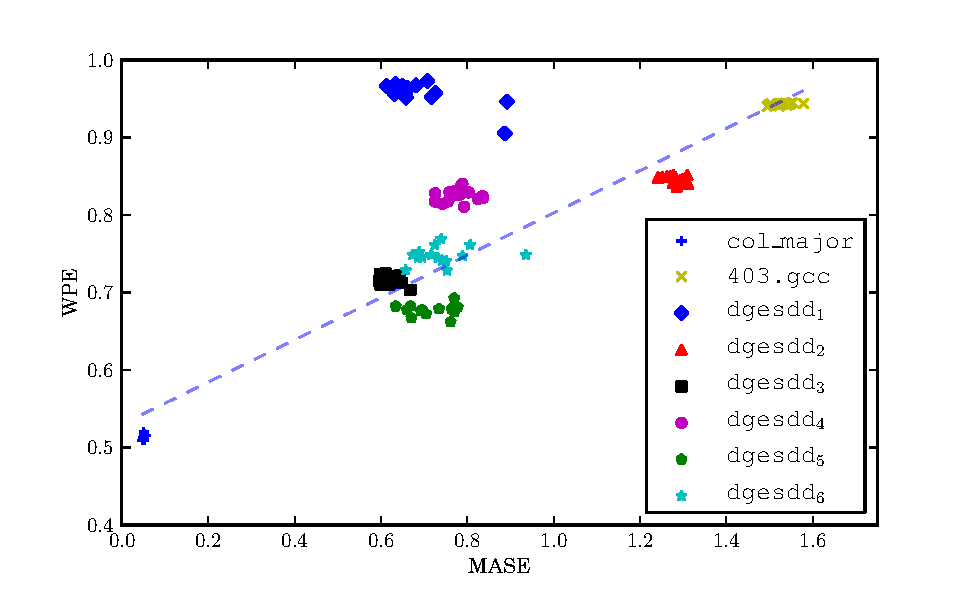
\includegraphics[width=1.1\columnwidth]{figs/new_prediction_vs_entropy}
  \caption{Weighted permutation entropy vs. mean absolute scaled error
    (MASE) of the best prediction of each time series.  The solid
    curve is a least-squares log fit of these points.
%
% of all the points except those from {\tt dgesdd$_1$}, which we have
% excluded for reasons explained in the text.
%
The dashed curves reflect the standard deviation of the model in its
parameter space.  The meaning of the shaded region is explained in the
text.}
  \label{fig:wpe_vs_mase_best}
\end{figure}
%
% As the plot shows, the best-case prediction error for each trace from
% these eight systems is roughly proportional to the log of the weighted
% permutation entropy, which is consistent with our first conjecture.
%
There is an obvious upward trend, which is consistent with the notion
that there is a pattern in the WPE-MASE relationship.  However, a
simple linear fit is a bad idea here.  First, any signal with zero
entropy should be perfectly predictable (i.e., MASE $\approx 0$), so
any curve fitted to these data should pass through the origin.
Moreover, WPE does not grow without bound, so one would expect the
patterns in the WPE-MASE pairs to reach some sort of asymptote.  For
these reasons, we chose to fit a function of the form $y = a \log(b x
+ 1)$ to these points, with $y =$ WPE and $x=$ MASE\footnote{The
  specific values of the coefficiencts are $a=7.97 \times 10^{-2}$ and
  $b=1.52 \times 10^3$.}.  The solid curve in the figure shows this
fit; the dashed curves show the standard deviation of this model in
its parameter space: i.e., $y = a \log(b x + 1)$ with $\pm$ one
standard deviation on each of the two parameters.  Points that fall
within this deviation volume (light grey) correspond to predictions
that are comparable to the best ones found in this study; points that
fall \emph{above} that volume (dark grey) are better still.  We chose
to truncate the shaded region because of a subtle point regarding the
MASE of an ideal predictor, which should not be larger than 1 unless
the training and test signals are different.  This is discussed at
more length below.

The curves and regions in Figure~\ref{fig:wpe_vs_mase_best} are a
graphical representation of the first finding.  This representation
is, we believe, a useful heuristic for determining whether a given
prediction method is well matched to a particular time series.  It is
not, of course, a formal result.  The forecast methods and data sets
used here were chosen to span the space of standard prediction
strategies and the range of dynamical behaviors, but they do not cover
those spaces exhaustively.  Our goal here is an \emph{empirical}
assessment of the relationship between predictability and complexity,
not formal results about a ``best'' predictor for a given time series.
There may be other methods that produce lower MASE values than those
in Figure~\ref{fig:wpe_vs_mase_best}, but the sparseness of the points
above and below the one-$\sigma$ region about the dashed curve in this
plot strongly suggests a pattern of correlation between the underlying
predictability of a time series and its WPE.  The rest of this section
describes these results and claims in more detail---including the
measures taken to assure meaningful comparisons across methods,
trials, and programs---and elaborates on the meaning of the different
curves and limits in the figure.

Figure~\ref{fig:wpe_vs_mase_all} shows WPE vs. MASE plots for the full
set of experiments.
\begin{figure*}
  \centering
%    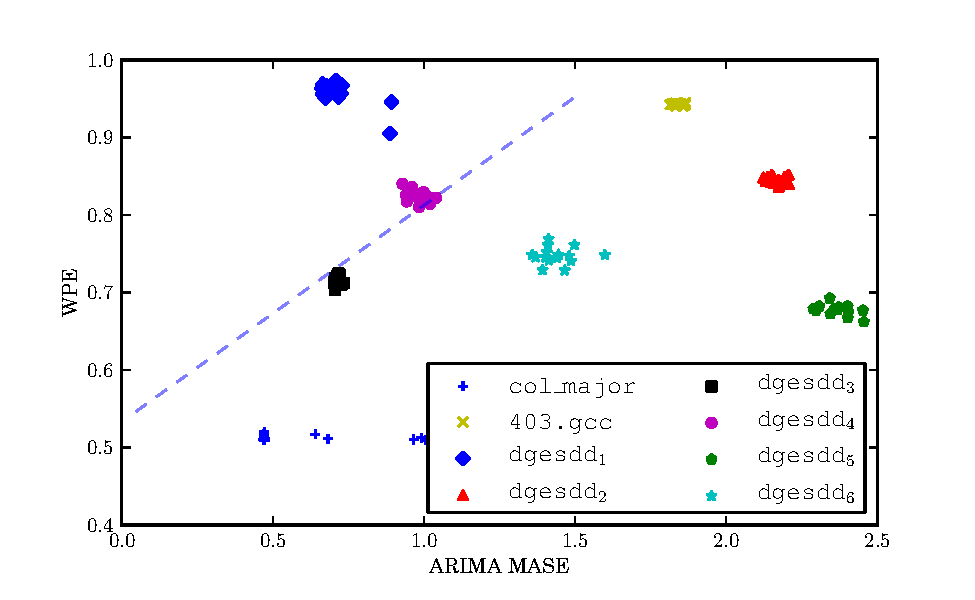
\includegraphics[width=\columnwidth]{figs/ARIMA_prediction_vs_entropy}
%    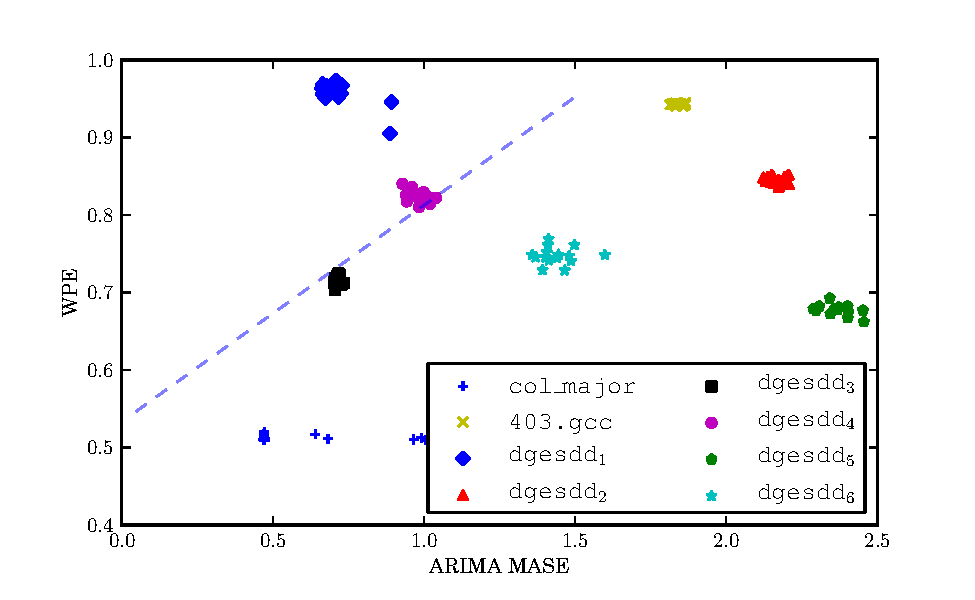
\includegraphics[width=\columnwidth]{figs/ARIMA_prediction_vs_entropy}
%    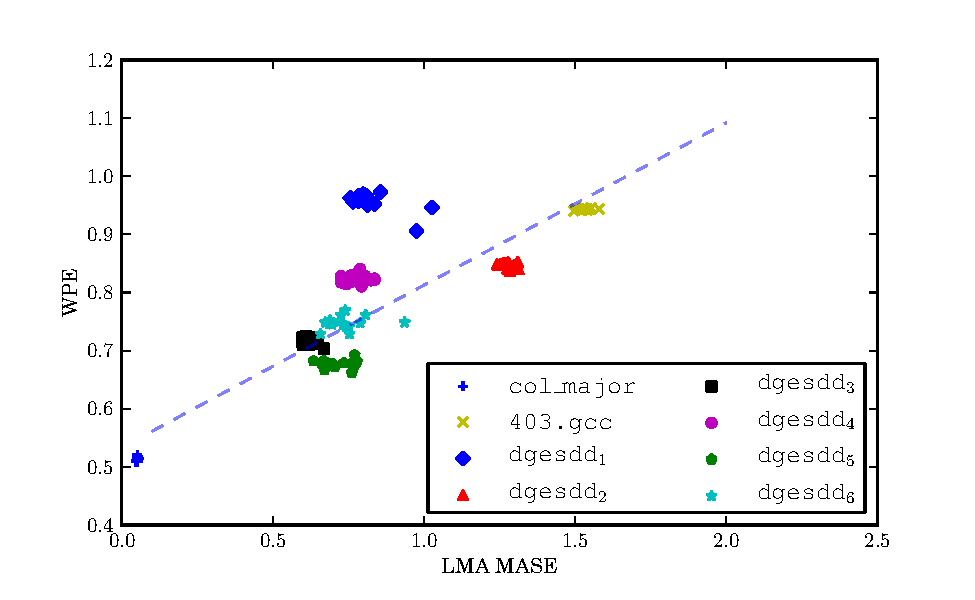
\includegraphics[width=\columnwidth]{figs/LMA_prediction_vs_entropy}
  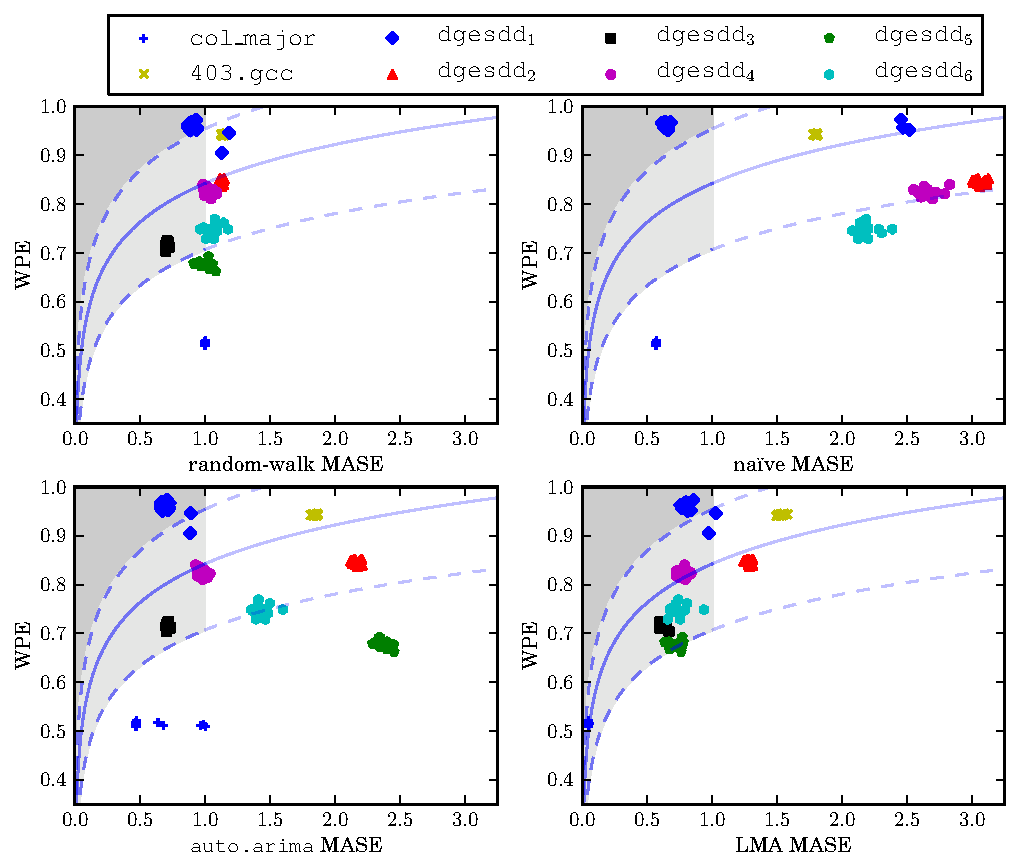
\includegraphics[width=1.7\columnwidth]{figs/new_predictions_vs_entropy4a}
\caption{WPE vs. MASE for all trials, methods, and systems---with the
  exception of \svdone, \svdthree, and \svdfive are omitted from the
  top-right plot for scale reasons, as described in the text.
%
% ; their MASE scores are $2.676 \pm 4.328$, $31.39 \pm 0.282$, and
%   $20.87 \pm 0.192$ respectively.
%
Numerical values, including means and standard deviations of the
errors, can be found in Table~\ref{tab:error}.  The curves and shaded
regions are the same as in the previous figure.  }
    \label{fig:wpe_vs_mase_all}
\end{figure*}
There are 15 points in each cluster, one for each trial.  (The points
in Figure~\ref{fig:wpe_vs_mase_best} are the leftmost of the points
for the corresponding trace in any of the four plots in
Figure~\ref{fig:wpe_vs_mase_all}.)  The WPE values do not vary very
much across trials.  For most traces, the variance in MASE scores is
low as well, resulting in small, tight clusters.  In some
cases---\arima predictions of {\tt col\_major}, for instance---the
MASE variance is larger, which spreads out the clusters horizontally.
The mean MASE scores of predictions generated with the nonlinear LMA
method, for instance, are generally closer to the dashed curve; the
\arima method clusters are more widely spread, the \naive ~clusters
even more so.  A few of the clusters have very high variance; these
are discussed later in this section.

The main thing to note here, however, is not the details of the shapes
of the clusters, but rather their positions in the four plots:
specifically, the fact that many of them are to the right of and/or
below the dashed curve that identifies the boundary of the shaded
region.  \emph{These predictions are not as good as our heuristic
  suggests they could be.}  Focusing in on any single cluster of
points makes this clear: LMA works best for \svdsix, for instance,
followed by the random-walk prediction method, then \arima and \naive.
When a practitioner calculates an WPE vs. MASE value that is outside the
shaded region, that should suggest to her that the prediction method
is not well matched to the task at hand: that is, the time series has
more predictive structure than the method is able to use.
%
% The idea behind the shaded region is to help practitioners identify
% when there is predictive structure in the data that a given method is
% not exploiting (viz., \arima on \svdsix)---i.e., that one could do
% better with another forecast strategy.
%
In this case---e.g., \arima on \svdsix---she should try a different
method.  The position of the LMA cluster for \svdsix, on the other
hand, reflects this method's ability to capture and exploit the
structure that is present in this signal.  WPE vs. MASE values like
this, which fall in the shaded region, should suggest to the
practitioner that the prediction method is well-suited to the task.
The following discussion lays out the details that underlie these
claims.
%
% The dashed curve in Figures~\ref{fig:wpe_vs_mase_best}
% and~\ref{fig:wpe_vs_mase_all} is a heuristic that captures the
% argument at the end of the previous paragraph.
%

Though \col is a very simple program, its dynamics are actually quite
complicated, as discussed in Section~\ref{sec:intro}.  Recall from
Figure~\ref{fig:forecast-example} and Table~\ref{tab:error} that the
\naive, \arima, and (especially) random-walk prediction methods do not
perform very well on this signal.  The MASE scores of these
predictions are $0.571 \pm 0.002$, $1.001 \pm 0.002$, and $0.599 \pm
0.211$, respectively, across all 15 trials.  That is, \naive ~and
\arima are performing only $\approx 1.7$ times better than the
random-walk method, a primitive strategy that simply uses the current
value as the prediction.  However, the WPE value for the \col trials
is $0.513 \pm 0.003$, which is in the center of the complexity
spectrum described in Section~\ref{sec:intro}.

This disparity---WPE values that suggest a high rate of forward
information transfer in the signal, but predictions with comparatively
poor MASE scores---is obvious in the geometry of the two left-hand
and the upper-right hand images in Figure~\ref{fig:wpe_vs_mase_all}, where the \col clusters
are far to the right of and/or below the dashed curve.  Again, this
indicates that these methods are not leveraging the available
information in the signal.  The dynamics of \col may be complicated,
but they are not unstructured.  This signal is nonlinear and
deterministic~\cite{mytkowicz09}, and if one uses a prediction
technique that is based a nonlinear model (LMA)---rather than a method
that simply predicts the running mean (\naive) or the previous value
(random walk), or one that uses a linear model (\arima)---the MASE
score is much better: $0.050 \pm 0.001$.  This prediction is 20 times
more accurate than a random-walk forecast, which is more in line with
the level of predictive structure that the low WPE value suggests is
present in the signal.  The MASE scores of random-walk predictions of
\col are all $\approx 1$---as one would expect---pushing those points
well below the shaded region.  Clearly the stationarity assumption on
which this method is based does not hold for this signal.

Note that the \col points (blue {\color{blue}$+$} icons) are clustered
very tightly in the lower left quadrant of the \naive, random-walk,
and LMA plots in Figure~\ref{fig:wpe_vs_mase_all}, but spread out
horizontally in the \arima plot.  This is because of the way the
\arima process builds ARIMA models \cite{autoARIMA}.  If a KPSS test
of the time series in question indicates that it is nonstationary, the
\arima recipe adds an integration term to the model.  This test gives
mixed results in the case of the \col process, flagging five of the 15
trials as stationary and ten as nonstationary.  ARIMA models without
an integration term perform more poorly on this signal, which
increases the error, thereby spreading out the points.  We tested this
hypothesis by forcing the inclusion of an integration term in the five
cases where a KPSS test indicated that such a term was not needed.
This action removed the spread, pushing all 15 of the \col ~ \arima
points in Figure~\ref{fig:wpe_vs_mase_all} into a tight cluster.
%\alert{Josh to do: this paragraph needs more, in response to the %ref's
%  gritch about fitting: the stuff about \arima being an automated
%  recipe that can give bad results, and the fact that our %technique
%  can tell when it does.  Look at the response letter for context %and
%  ammunition---and also put something in there that calls his
%  attention to this paragraph.}

The discussion in the previous paragraph highlights the second finding
of this paper: the ability of our proposed heuristic to flag
inappropriate models.  \arima is an automated, mechanical procedure
for choosing parameters for an ARIMA model of a given data set.  While
the tests and criteria employed by this algorithm are sophisticated
(see Section~\ref{sec:arima}), the results can still be
sub-optimal---if the initial space of models being searched is not
broad enough, for instance, or if one of the preliminary tests gives
an erroneous result.  \arima \emph{always} returns a model, and it can
be very hard to detect when that model is bad.  Our results suggest a
way to do so: if the MASE score of an \arima model is out of line with
the WPE value, that can be an indication of inappropriateness in the
order selection and parameter estimation procedure.  By examining the
\arima MASE scores vs. WPE values of \col, we were able to see that,
while all signal complexities were the same, some of the signals had
much higher MASE values. This suggested to us inappropriate parameter
selection for these time series. We then went back and manually
assisted the automated fitting procedure, resulting in models with
consistent MASE vs WPE score, and improved forecasts.

% The discussion in the previous paragraph brings to light an
% interesting feature of our proposed heuristic. The \arima algorithm
% that was used to build all of the ARIMA models in this paper follows
% the procedure outlined in Section V B to choose values for the model
% parameters.  As discussed previously, this algorithm employs
% sophisticated tests, such as the KPSS test, to intelligently traverse
% and reduce model space and then uses well-known criterion for choosing
% the most-likely of the remaining models. However, it is quite possible
% that this procedure can choose a sub-optimal fit. Specifically, if the
% initial space of models being searched is not broad enough, or if one
% of the preliminary tests gives an erroneous result, then the best
% ARIMA model may be excluded or eliminated before likelihood is even
% examined. This circumstance is hard to detect. Maximal-likelihood
% tests, such as AIC used in \arima, can only conclude which of the
% models provided is ``most likely"---but cannot conclude that
% \emph{none} of the models are likely. In contrast,
% %Sometimes the choices made by that procedure produce a sub-optimal predictor, however there is nothing to say whether a different model from the ARIMA class would work better.
% inappropriate MASE scores (compared to what the WPE value might
% suggest) may suggest an inappropriateness in the order selection and
% parameter estimation procedure, which would flag to a practitioner to
% reevaluate the appropriateness of fit. For example,
% %During the fitting process of \arima many subclasses of ARIMA models are eliminated based on various tests, such as the KPSS test. If these tests give erroneous results then entire subclasses of ARIMA models are never even considered. Our heuristic may be able to flag when this has occurred.
% by examining the \arima MASE scores vs. WPE values of \col, we were
% able to see that, while all signal complexities were the same, some of
% the signals had much higher MASE values. This suggested to us
% inappropriate parameter selection for these time series. We then went
% back and manually assisted the automated fitting procedure, resulting
% in models with consistent MASE vs WPE score, and improved forecasts.

The WPE of \svdfive ($0.677 \pm 0.006$) is higher than that of {\tt
  col\_major}.  This indicates that the rate of forward information
transfer of the underlying process is lower, but that time-series data
observed from this system still contain a significant amount of
structure that can, in theory, be used to predict the future course of
the time series.
% As mentioned above, though, the effectiveness of any prediction
% strategy depends on how well it leverages the information that is
% available in the data: methods that use linear models, for instance,
% may fail when applied to nonlinear processes.  (This is the basis
% for the second conjecture above.)
The MASE scores of the \naive ~and \arima predictions for this system
are $20.870 \pm 0.192$ and $2.370 \pm 0.051$, respectively: that is,
20.87 and 2.37 times worse than a simple random walk forecast of the
same signals\footnote{The \naive ~MASE score is large because of the
  bimodal nature of the distribution of the values of the signal,
  which makes guessing the mean a particularly bad strategy.  The same
  thing is true of the \svdthree signal.}.  As before, the positions
of these points on a WPE vs. MASE plot---significantly below and to
the right of the shaded region---should suggest to a practitioner that
%  there is more structure in this signal than the corresponding
% method is able to leverage, and that
a different method might do better.  Indeed, for \svdfive, the LMA
method produces a MASE score of $ 0.718\pm 0.048 $ and a cluster of
results that largely within the shaded region on the WPE-MASE plot.
This is consistent with our second finding: the LMA method can capture
and reproduce the way in which the \svdfive system processes
information, but the \naive ~and \arima prediction methods cannot.

The WPE of \gcc is higher still: $0.943 \pm 0.001$.  This system
transmits very little information forward in time and provides almost
no structure for prediction methods to work with.  Here, the
random-walk predictor is the best of the methods used here.  This
makes sense; in a fully complex signal, where there is no predictive
structure to utilize, methods that depend on exploiting that
structure---like ARIMA and LMA---will be outperformed by methods that
do not rely on that structure.
%
% in a fully complex signal, the MASE of a random-walk forecast will
% always be $\approx 1$, assuming that the training signal accurately
% reflects the overall behavior of the out-of-sample time series
%
Since fitting a hyperplane using least squares should filter out some
of the noise in the signal, the fact that LMA outperforms \arima
($1.530 \pm 0.021$ vs. $1.837 \pm 0.016$) may be somewhat
counterintuitive.  However, the small amount of predictive structure
that is present in this signal is nonlinear (cf.,~\cite{mytkowicz09}),
and LMA is designed to capture and exploit that kind of structure.
Note that all four \gcc clusters in Figure~\ref{fig:wpe_vs_mase_all}
are outside the shaded region; in the case of the random-walk
prediction, for instance, the MASE value is $1.1381 \pm 0.011$.  This
is due to nonstationarity in the signal: in particular, differences
between the training and test signals.  \svdtwo fits the same
patterns, for the same reasons---and visibly so, in the red segment of
Figure~\ref{fig:svd-ts-colored}, where the period and amplitude of the
oscillations are decreasing.

\svdone---the dark blue segment of
Figure~\ref{fig:svd-ts-colored}---behaves very differently than the
other seven systems in this study.  Though its weighted permutation
entropy is very high ($0.957 \pm 0.016$), three of the four prediction
methods do quite well on this signal, yielding mean MASE scores of
0.714 (\arima), 0.827 (LMA), and 0.933 (random walk).  This pushes the
corresponding clusters of points in Figure~\ref{fig:wpe_vs_mase_all}
well above the trend followed by the other seven signals.  The reasons
for this are discussed in the following paragraph.  The MASE scores of
the predictions that were produced by the \naive ~method for this
system, however, are highly inconsistent.  The majority of the blue
diamond-shaped points on the top-right plot in
Figure~\ref{fig:wpe_vs_mase_all} are clustered near a MASE score of
0.6, which is better than the other three methods.  In five of the 15
\svdone trials, however, there were step changes in the signal.  The
\naive ~method has a very difficult time with signals like this,
particularly if there are multiple step changes.  This raised the MASE
scores of these trials, pushing the corresponding points to the
right\footnote{This includes the cluster of three points near MASE
  $\approx 2.5$, as well as two points that are beyond the domain of
  the graph, at MASE $\approx 11.2-14.8$.}, and in turn raising both
the mean and variance of this set of trials.

The effects described in the previous paragraph are also exacerbated
by the way MASE is calculated.  Recall that MASE scores are scaled
\emph{relative to a random-walk forecast of the training set}.  There
are two issues here.  First, random-walk prediction works very badly
on signals with frequent, large, rapid transitions.  Consider a signal
that oscillates from one end of its range to the other at every step.
A signal like this will have a low WPE, much like {\tt col\_major}.
However, a random-walk forecast of this signal will be 180 degrees out
of phase with the true continuation.  Since random-walk error appears
in the denominator of the MASE score, this effect can shift points
leftwards on a WPE vs. MASE plot, and that is exactly why the \svdone
clusters in Figure~\ref{fig:wpe_vs_mase_all} are above the dashed
curve.  This time series, which is shown in closeup in
Figure~\ref{fig:svdone-ts},
\begin{figure}[htbp]
  \centering
    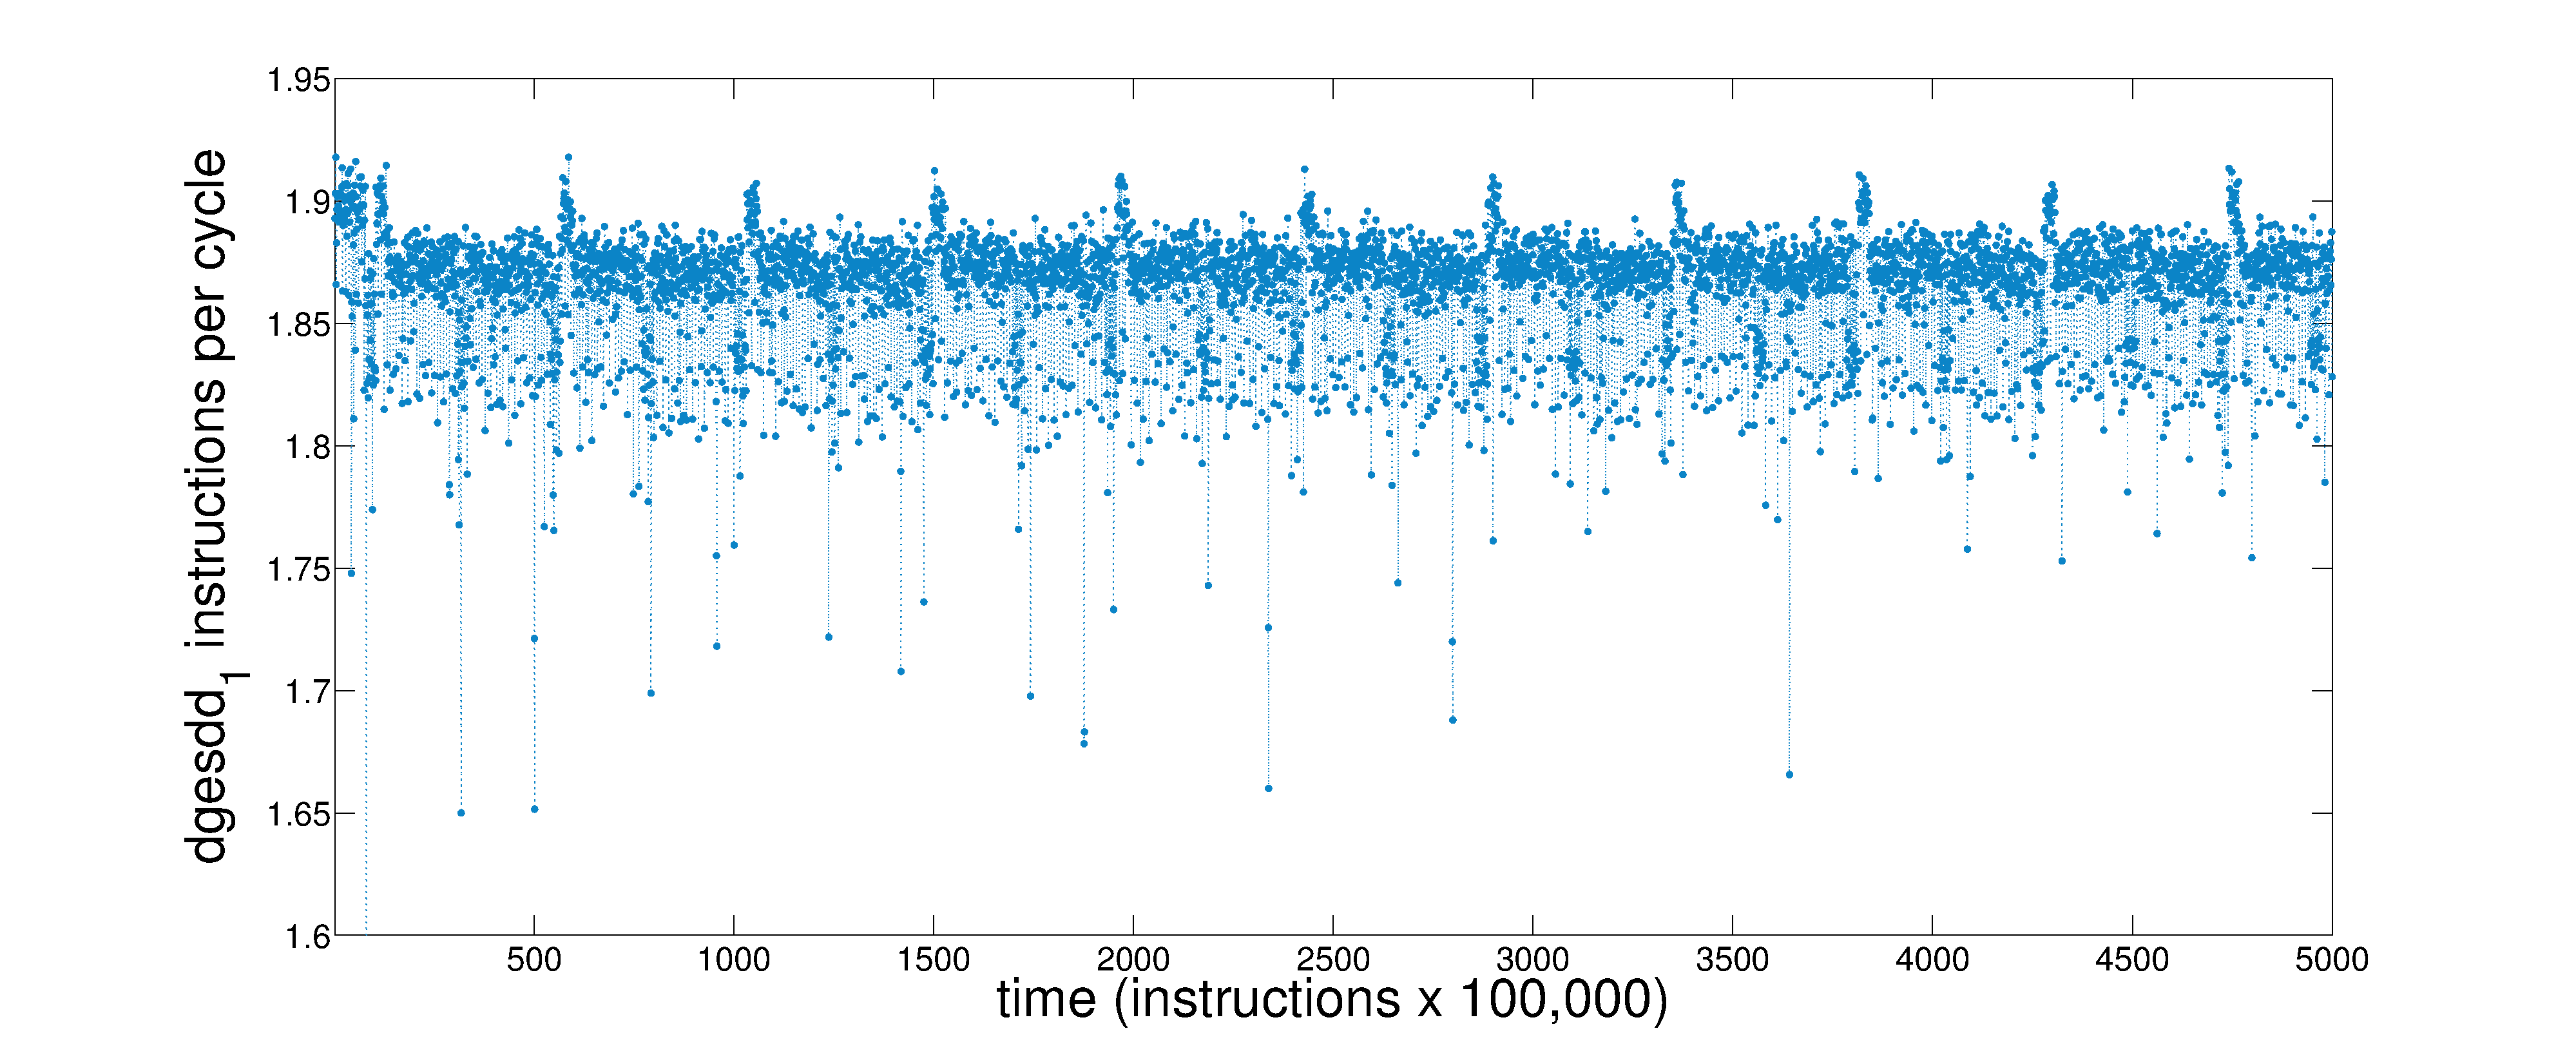
\includegraphics[width=\columnwidth]{figs/svdonets2}
\caption{A small portion of the \svdone time series}\label{fig:svdone-ts}
\end{figure}
is not quite to the level of the worst-case signal described above,
but it still poses a serious challenge to random-walk prediction.  It
is dominated by a noisy regime (between $\approx$1.86 and
$\approx$1.88 on the vertical scale in Figure~\ref{fig:svdone-ts}),
punctuated by short excursions above 1.9.  In the former regime, which
makes up more than 80\% of the signal, there are frequent dips to 1.82
and occasional larger dips below 1.8.  These single-point dips are the
bane of random-walk forecasting.  In this particular case, roughly
40\% of the forecasted points are off by the width of the associated
dip, which skews the associated MASE scores.  Signals like this are
also problematic for the \naive ~prediction strategy, since the
outliers have significant influence on the mean.  This compounds the
effect of the skew in the scaling factor and exacerbates the spread in
the \svdone MASE values.

% For all of these reasons, we view \svdone as an outlier and exclude it
% from the fit calculation of the dashed curve in
% Figure~\ref{fig:wpe_vs_mase_best}.

The second effect that can skew MASE scores is nonstationarity.  Since
this metric is normalized by the error of a random-walk forecast
\emph{on the training signal}, differences between the test signal and
training signal can create issues.  This is why the MASE values in
Table~\ref{tab:error} are not identically one for every random-walk
forecast of every time series: the last 10\% of these signals is
significantly different from the first 90\%.  The deviation from 1.00
will depend on the process---whether it has multiple regimes, what
those regimes look like, and how it switches between them---as well as
the experimental setup (e.g., sensor precision and data length).  For
the processes studied here, these effects do not cause the MASE values
to exceed 1.15, but pathological situations (e.g., a huge switch in
scale right at the training/test signal boundary) could produce higher
values.  This suggests another potentially useful heuristic: if the
MASE of a random-walk prediction of a time series is significantly
different from 1, this could be an indication that the signal is
nonstationary.  We are in the process of exploring this idea.

Again, the curves in Figures~\ref{fig:wpe_vs_mase_best}
and~\ref{fig:wpe_vs_mase_all} were determined from a finite set of
methods and data.  We put a lot of thought and effort into making
these experiments upon which these results are based both
representative and comprehensive.  The forecast methods involved range
from the simple to the sophisticated; the time-series data was sampled
from a system whose behavior spans the dynamical behavior space.
While we are cautiously optimistic about the generality of our
conclusions, more exploration will be required before we can make any
such claim.  Our preliminary work along those lines shows that data
from the Henon map \cite{henon}, the Lorenz system \cite{lorenz}, and
the SFI A data set \cite{weigend-book,sfi-data} all fall within the
one-$\sigma$ volume of the fit in Figures~\ref{fig:wpe_vs_mase_best}
and~\ref{fig:wpe_vs_mase_all} region, as do various nonlinear
transformations of \svdtwo, \svdfive and \svdsix.

Of course, the geometry of these curves and bounds do not necessarily
extend to other error metrics.  The positions of the WPE vs. error
points---and the reasons to choose a particular function to fit to
them or impute theoretical bounds on the meaning of the results---may
change if one calculates error using a procedure other than the one
described in Section~\ref{sec:accuracy}.  The MASE error metric, as
discussed above, has its weaknesses.  Even so, we concur with
\cite{MASE} that it is an effective way to compare prediction error
across time-series data of different lengths and different scales, and
we are convinced by the extensive evaluations that are offered in that
paper, as well as the comparisons of MASE to other metrics, that its
strengths far outweigh its weaknesses.

%This portion should justify the following claim%%%%%%%%%%%%%%%%%%%%%%
%\item The way structure/information/complexity is processed internally by a given process plays a crucial role in predictability.
%%%%%%%%%%%%%%%%%%%%%%%%%

%In Figures~\ref{fig:lma_pred_vs_ent} and \ref{fig:arima_pred_vs_ent} we directly compare the performance of the LMA and ARIMA prediction methods (respectively) to the value of the weighted permutation entropy for all runs of each program under consideration. The LMA MASE values are largely similar to those of the best predictions, primarily because LMA often performed superior to ARIMA (and the na\"ive method). On the other hand, the ARIMA MASE values are largely uncorrelated with WPE values. As was hinted at while discussing the previous results, the fact that ARIMA is uncorrelated with WPE brings about an interesting perspective on information transfer and WPE. The WPE is sensitive to both linear and nonlinear structure. When you have a low WPE and a high ARIMA it could be that the structure WPE is picking up is simply nonlinear structure that LMA can handle but ARIMA cannot. So while ARIMA is consistently out performed by random walk,  there is plenty of structure present as suggested by WPE and taken advantage of by LMA but since it is nonlinear ARIMA can't take it into account and does bad.



%is in large part one of the major findings of this work. More specifically, say we tried to predict an arbitrary noisy real-valued time series with an ``out-of-the-box" prediction strategy like ARIMA as proposed in \cite{autoArima} and say we got inconsistent and bad forecasts, (i.e., perform worse than the na\"ive random walk strategy ($MAS>1$). How do we determine if the prediction strategy is not adequate for the prediction task, or if the signal is simply too complex to predict. If a signal is too complex and too little forward information transfer is present we may not be able to do better than the random walk, in which case we should not worry ourselves over finding a more complicated prediction strategy. However, if we measure the complexity to be low, $\textrm{WPE}<0.85$ (see Fig.~\ref{fig:pred_vs_wpe}) we can most likely do much better than the random walk and should search for more adequate prediction strategies.




\section{ Conclusions \& Future Work }\label{sec:conc}

% To address the shortcomings mentioned in the previous section, we are
% in the process of repeating our own study with other metrics, other
% forecast methods, and time-series data from other systems.

Forecast strategies that are designed to capture predictive structure
are ineffective when signal complexity outweighs information
redundancy.  This poses a number of serious challenges in practice.
Without knowing anything about the generating process, it is difficult
to determine how much predictive structure is present in a noisy,
real-world time series.  And even if predictive structure exists, a
given forecast method may not work, simply because it cannot exploit
the structure that is present (e.g., a linear model of a nonlinear
process).  If a forecast model is not producing good results, a
practitioner needs to know why: is the reason that the data contain no
predictive structure---i.e., that no model will work---or is the model
that s/he is using simply not good enough?

In this paper, we have argued that redundancy is a useful proxy for
the inherent predictability of an empirical time series.  To
operationalize that relationship, we use an approximation of the
Kolmogorov-Sinai entropy, estimated using a weighted version of the
permutation entropy of~\cite{bandt2002per}.  This WPE technique---an
ordinal calculation of forward information transfer in a time
series---is ideal for our purposes because it works with real-valued
data and is known to converge to the true entropy value. Using a
variety of forecast models and more than 150 time-series data sets
from experiments and simulations, we have shown that prediction
accuracy is indeed correlated with weighted permutation entropy: the
higher the WPE, in general, the higher the prediction error.  The
relationship is roughly logarithmic, which makes theoretical sense,
given the nature of WPE, predictability, and MASE.

An important practical corollary to this empirical correlation of
predictability and WPE is a practical strategy for assessing
appropriateness of forecast methods.  If the forecast produced by a
particular method is poor but the time series contains a significant
amount of predictive structure, one can reasonably conclude that that
method is inadequate to the task and that one should seek another
method.  The nonlinear LMA method, for instance, performs better in
most cases because it is more general.  (This is particularly apparent
in the \col and \svdfive examples.)
% , where the other two methods do not perform well.)
The \naive ~method, which simply predicts the mean, can work very well
on noisy signals because it effects a filtering operation.  The simple
random-walk strategy outperforms LMA, \arima, and the \naive
~method on the \gcc signal, which is extremely complex---i.e.,
extremely low redundancy.
%  \naive ~wins on \svdone with the exception to the 5 outliers.

The curves and shaded regions in Figures~\ref{fig:wpe_vs_mase_best}
and~\ref{fig:wpe_vs_mase_all} generalize and operationalize the
discussion in the previous paragraph.  These geometric features are a
preliminary, but potentially useful, heuristic for knowing when a
model is not well-matched to the task at hand: a point that is below
and/or to the right of the shaded regions on a plot like
Figure~\ref{fig:wpe_vs_mase_all} indicates that the time series has
more predictive structure than the forecast model can capture and
exploit---and that one would be well advised to try another method.

These curves were determined empirically using a specific error metric
and a finite set of forecast methods and time-series traces.  If one
uses a different error metric, the geometry of the heuristic will be
different---and may not even make sense, if one uses a metric that
does not support comparison across different time series.  And while
the methods and traces used in this study were chosen to be
representative of the practice, they are of course not completely
comprehensive.  It is certainly possible, for instance, that the
nonlinear dynamics of computer performance is subtly different from
the nonlinear dynamics of other systems.  Our preliminary results on
other systems (H\'enon, Lorenz, a random-walk process, SFI ``A'',
nonlinear transformations of the computer performance data) lead us to believe
that our results will generalize beyond the examples described in this
paper.  We are in the process of following up on that exploration with
a broader study of data, forecast methods, and error metrics.

% {\color{blue}agreed, I don't think it addds anything}\alert{I'm not
%   sure this paragraph adds anything.  Can/should we remove it?  Given
%   that information is a fundamental limitation in predictability, then
%   gathering and using more information is an obvious next step.  But
%   there is an equally obvious tension here between data length and
%   prediction speed: a forecast that requires half a second to compute
%   is not useful for the purposes of real-time control of a computer
%   system with a MHz clock rate, for instance.  Another alternative is
%   to sample several system variables simultaneously and build
%   multivariate models.  This is a particular challenge in nonlinear
%   LMA-type models, since multivariate delay-coordinate embedding
%   (e.g., \cite{cao-multivariate-embedding,deyle-sugihara2011}) can be
%   computationally prohibitive.  We are working on alternative methods
%   that sidestep that complexity.}
%

%Paragraphs on the issues that come up, including one about the "amount
%of info" one: if one could sample more variables, for instance, one
%might be able to do a better job of predicting more-complex traces.
%Segue to some handwaving about multivariable LMA models; tie this back
%to the "computers are NLD systems" stuff in the intro.  This is a real
%challenge; current approaches to this modelling problem have the major
%issue of taking way too long to build.  And that's a big issue if
%you're trying not just to classify, but to predict.  In a system that
%runs at MHz speeds, a prediction that takes milliseconds to compute is
%not useful.
%\end{it}

Nonstationarity is a serious challenge in any time-series modeling
problem.  Any regime shift that causes a change in the predictive
structure between the training signal and the test signal, for
instance, may skew the MASE score and thereby affecting the utility of
our heuristic.  Conversely, though, a MASE score of a random-walk
prediction that is significantly different from 1.0---as mentioned at
end of the previous section---could potentially be a good indicator of
nonstationarity.

Detecting regime shifts---and adapting prediction models
accordingly---is an important area of future work.  Indeed, one of the
first applications of permutation entropy was to recognize the regime
shift in brainwave data that occurs when someone has a
seizure~\cite{cao2004det}.  Recall that the signal in
Figure~\ref{fig:svd-ts-colored} was especially useful for the study in
this paper because it contained a number of different regimes.  We
segmented this signal visually, but one could imagine using some
combination of WPE and MASE to do so instead (e.g., in a sliding
window across the time series).  Automating regime-shift detection
would be an important step towards a fully adaptive modeling strategy,
where old models are discarded and new ones are rebuilt whenever the
time series enters a new regime.  Our WPE vs. MASE results could be
particularly powerful in this scenario, as their values could not only
help with regime-shift detection, but also suggest what kind of model
might work well in each new regime.  Of particular interest would be
the class of so-called \emph{hybrid systems}~\cite{hybrid}, which
exhibit discrete transitions between different continuous
regimes---e.g., a lathe that has an intermittent instability or
traffic at an internet router, whose characteristic normal traffic
patterns shift radically during an attack.  Effective modeling and
prediction of these kinds of systems is quite difficult; doing so
adaptively and automatically---in the manner that is alluded to at the
end of the previous paragraph---would be an interesting challenge.






\section*{Acknowledgment}
This work was partially supported by NSF grant \#CMMI-1245947 and ARO
grant \#W911NF-12-1-0288.

\section{Appendix}

\begin{table}[h]
  \begin{center}
  \begin{tabular}{|c|c|c|c|c|}
  \hline
            & MASE LMA    & MASE ARIMA &MASE na\"{i}ve   & $l=6$ \\
 \hline 
 
 \col           & $ 0.050 \pm0.002  $ & $0.599  \pm 0.211 $ & $0.571\pm0.002$&  $0.513 \pm 0.003$ \\

\gcc           & $ 1.530\pm 0.021$ & $1.837 \pm0.016 $ & $0.951 \pm 0.001$ & $0.943 \pm 0.001$ \\

\svdone     & $ 0.827\pm 0.076$ & $ 0.714\pm 0.075 $ & $2.676\pm4.328$&  $0.957 \pm 0.016$ \\

 \svdtwo    & $1.279 \pm0.020 $ & $2.163 \pm0.027 $ &  $3.054\pm0.040$ &   $0.846 \pm0.004$ \\
 
 \svdthree     & $0.619 \pm0.021 $ & $0.713 \pm 0.010 $ & $31.386\pm 0.282$ &  $0.716 \pm 0.006$ \\

 \svdfour     & $ 0.779\pm0.036 $ & $0.979 \pm0.032 $ & $2.661\pm0.074$ & $0.825 \pm 0.008$ \\
 
 \svdfive     & $ 0.718\pm 0.048 $ & $2.370  \pm 0.051 $ & $20.870 \pm 0.192$&  $0.678 \pm 0.007$ \\
 
 \svdsix     & $ 0.739\pm 0.068 $ & $ 1.438\pm 0.0610$ & $2.197\pm0.083$&  $0.748 \pm 0.011$ \\
  \hline
  \end{tabular}
  \end{center}
 \label{default}
 \caption{Detailed MASE scores}
 \label{tab:error}
  \end{table}%




\bibliographystyle{aipauth4-1}
\bibliography{bibliofile}


\end{document}
